\subsection{Lepton MVA sideband region}

The 2lss selection is modified by requiring that only one of the two selected leptons fails the tight lepton requirements, but still passes those for the fakeable object. In this way, we select a region enriched in $\ttbar$ events, where the lepton that fails the tight requirement is a fake lepton.

It is worth noting that the contamination from QCD events is not taken into account by the simulation. We observe a good agreement between simulation and data in terms of the shape of observables used for the selection and as inputs to the BDT discriminators. The latter variables are shown in Fig.~\ref{fig:cr_2lss_appl_1fo_3}.

\begin{figure}[!htb]
\centering
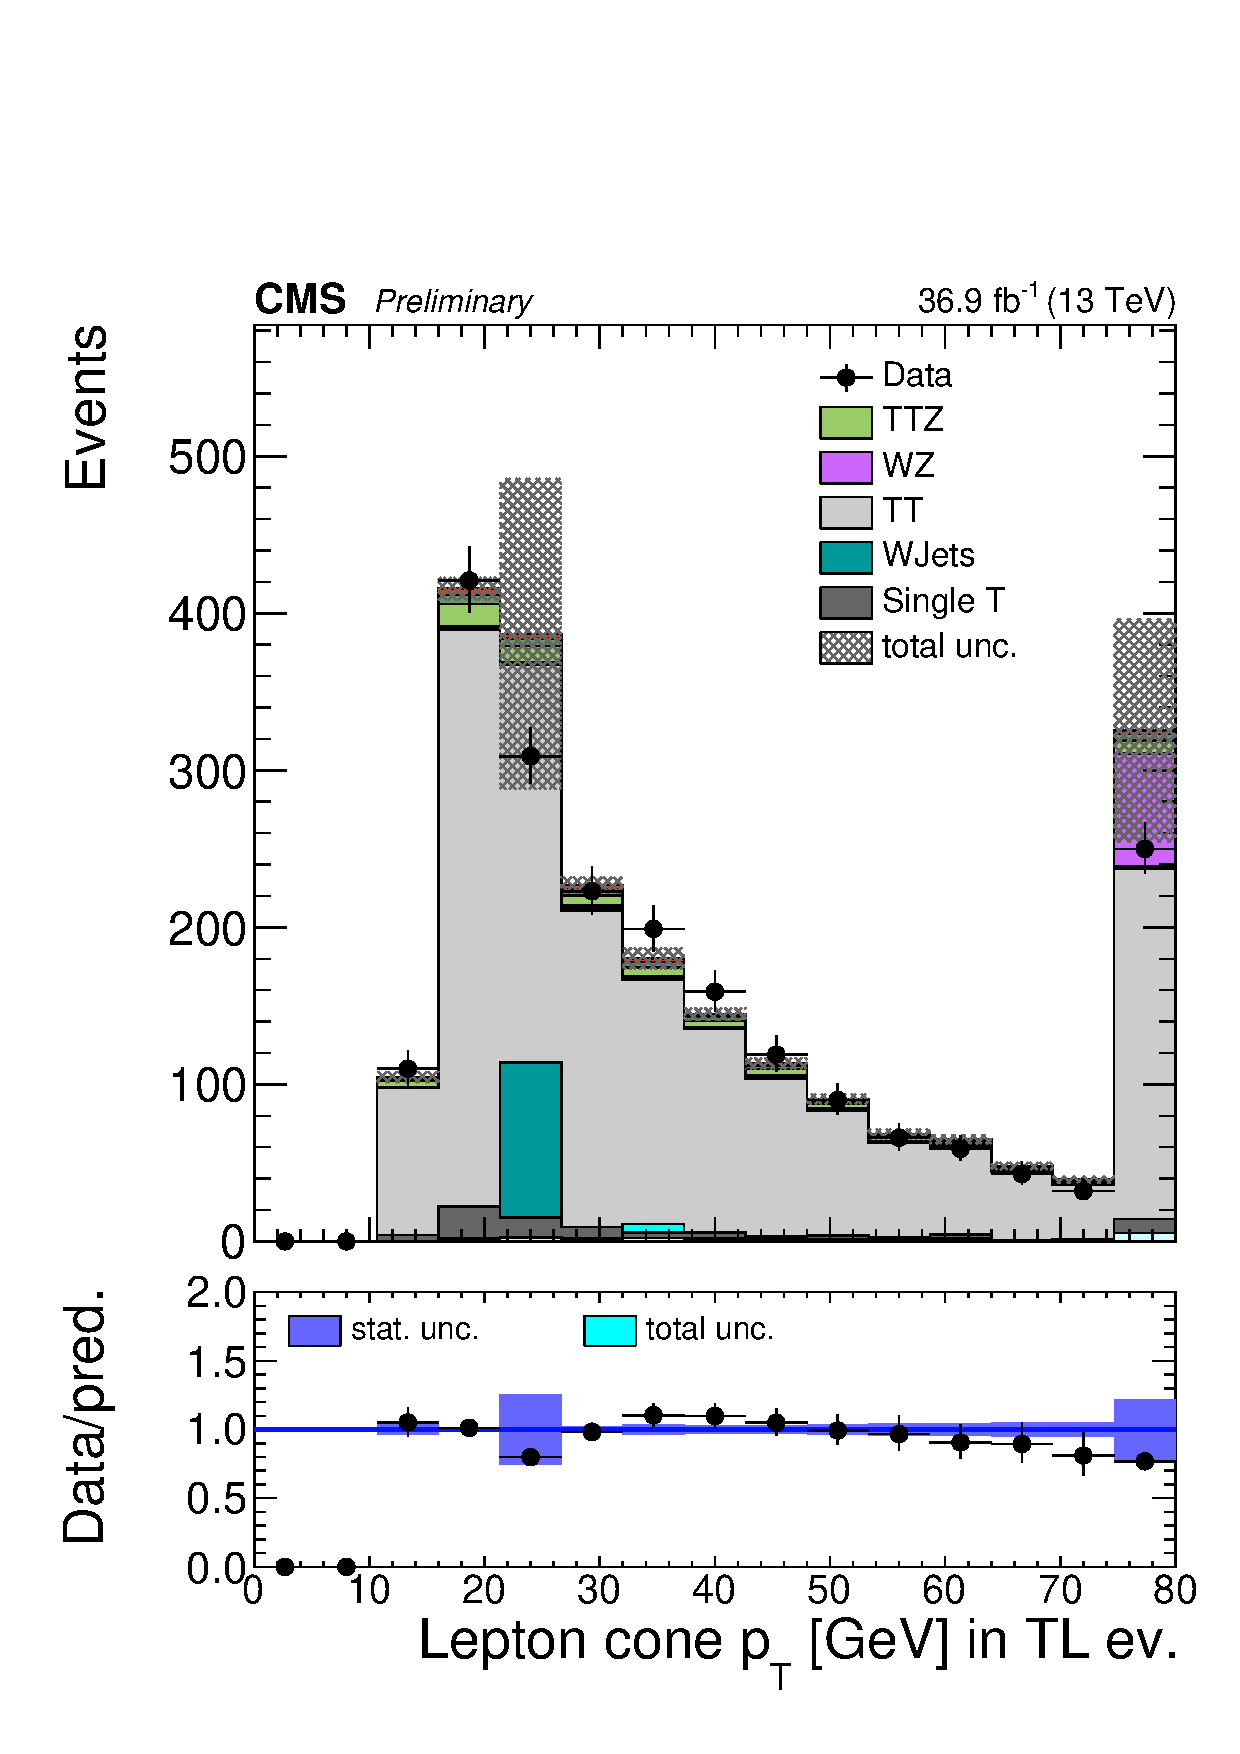
\includegraphics[width=0.30\linewidth]{plots_controlregions/2lss_appl_1fo_data/nT_2lep_conePt.pdf}
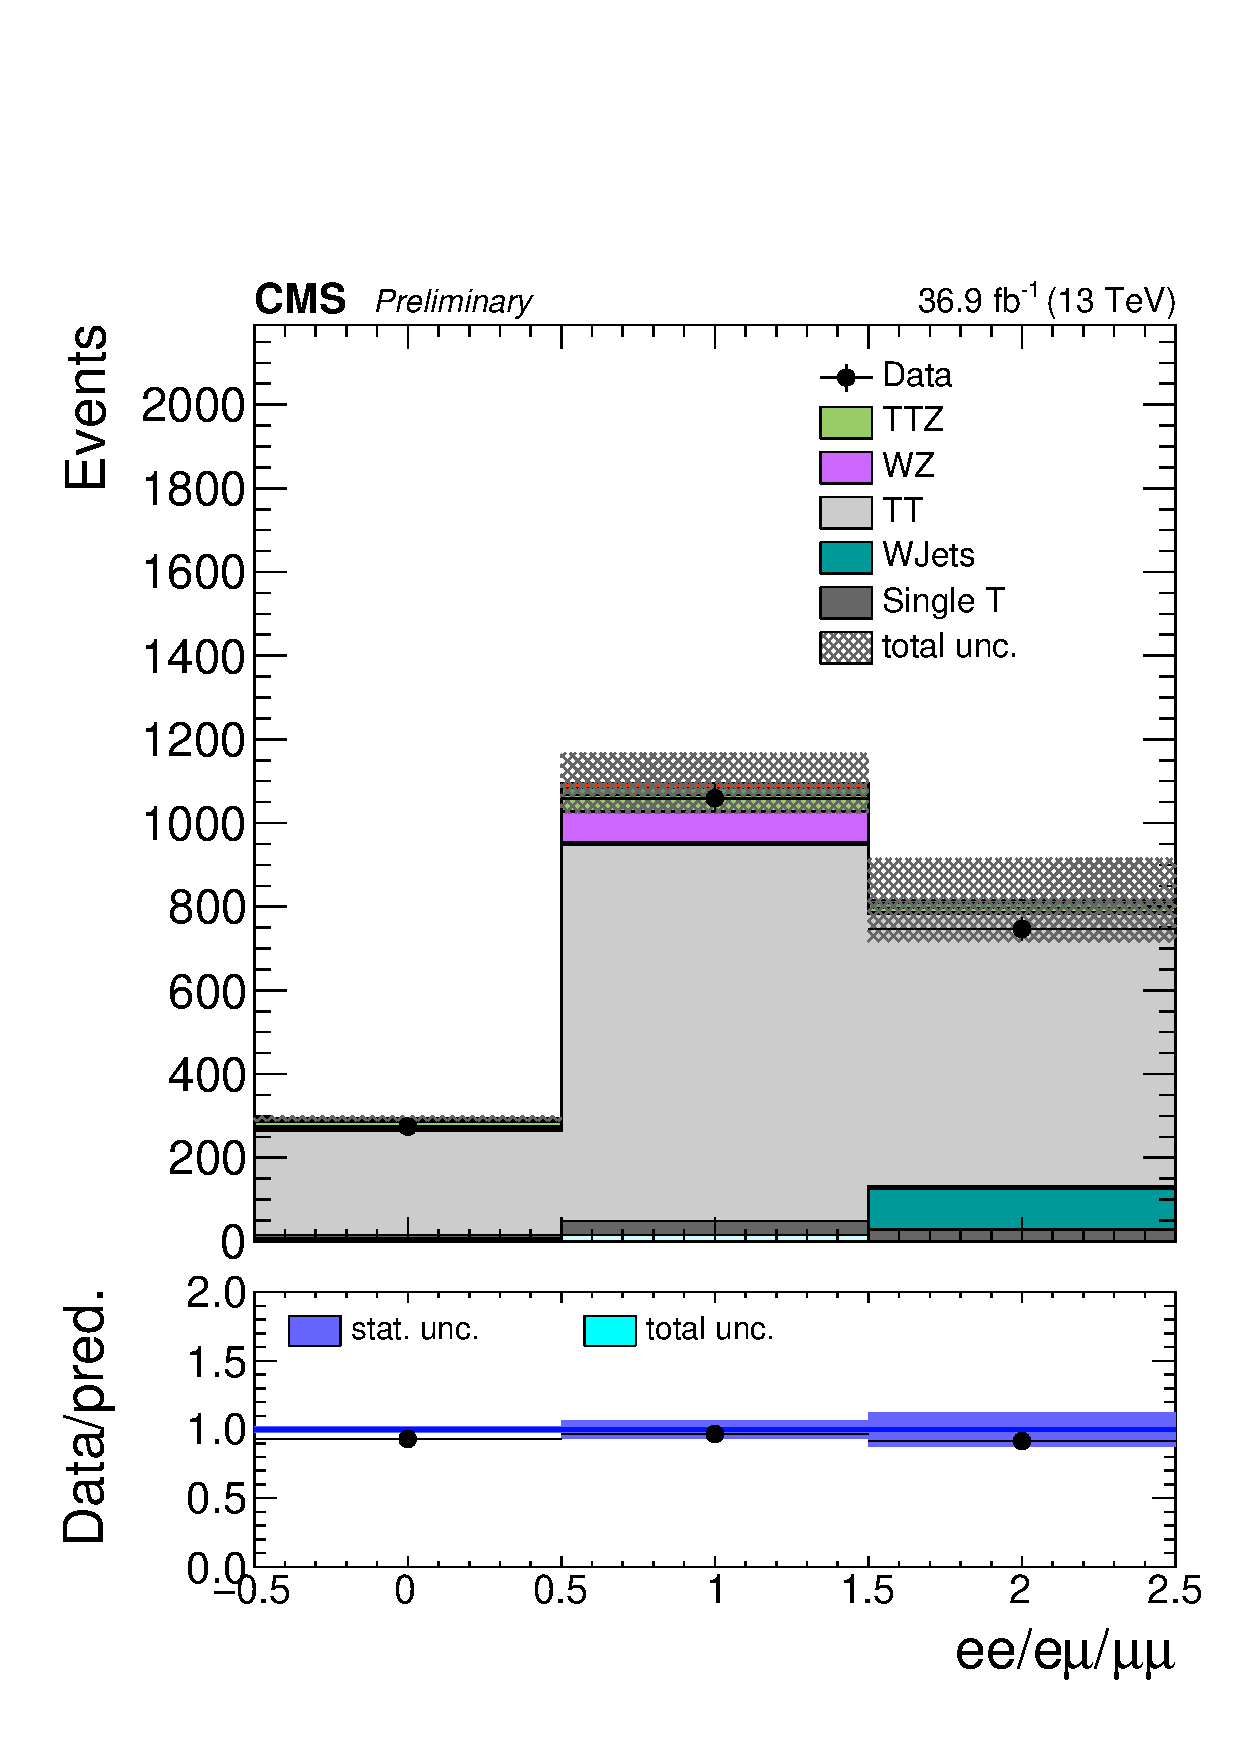
\includegraphics[width=0.30\linewidth]{plots_controlregions/2lss_appl_1fo_data/2lep_flav.pdf}\\
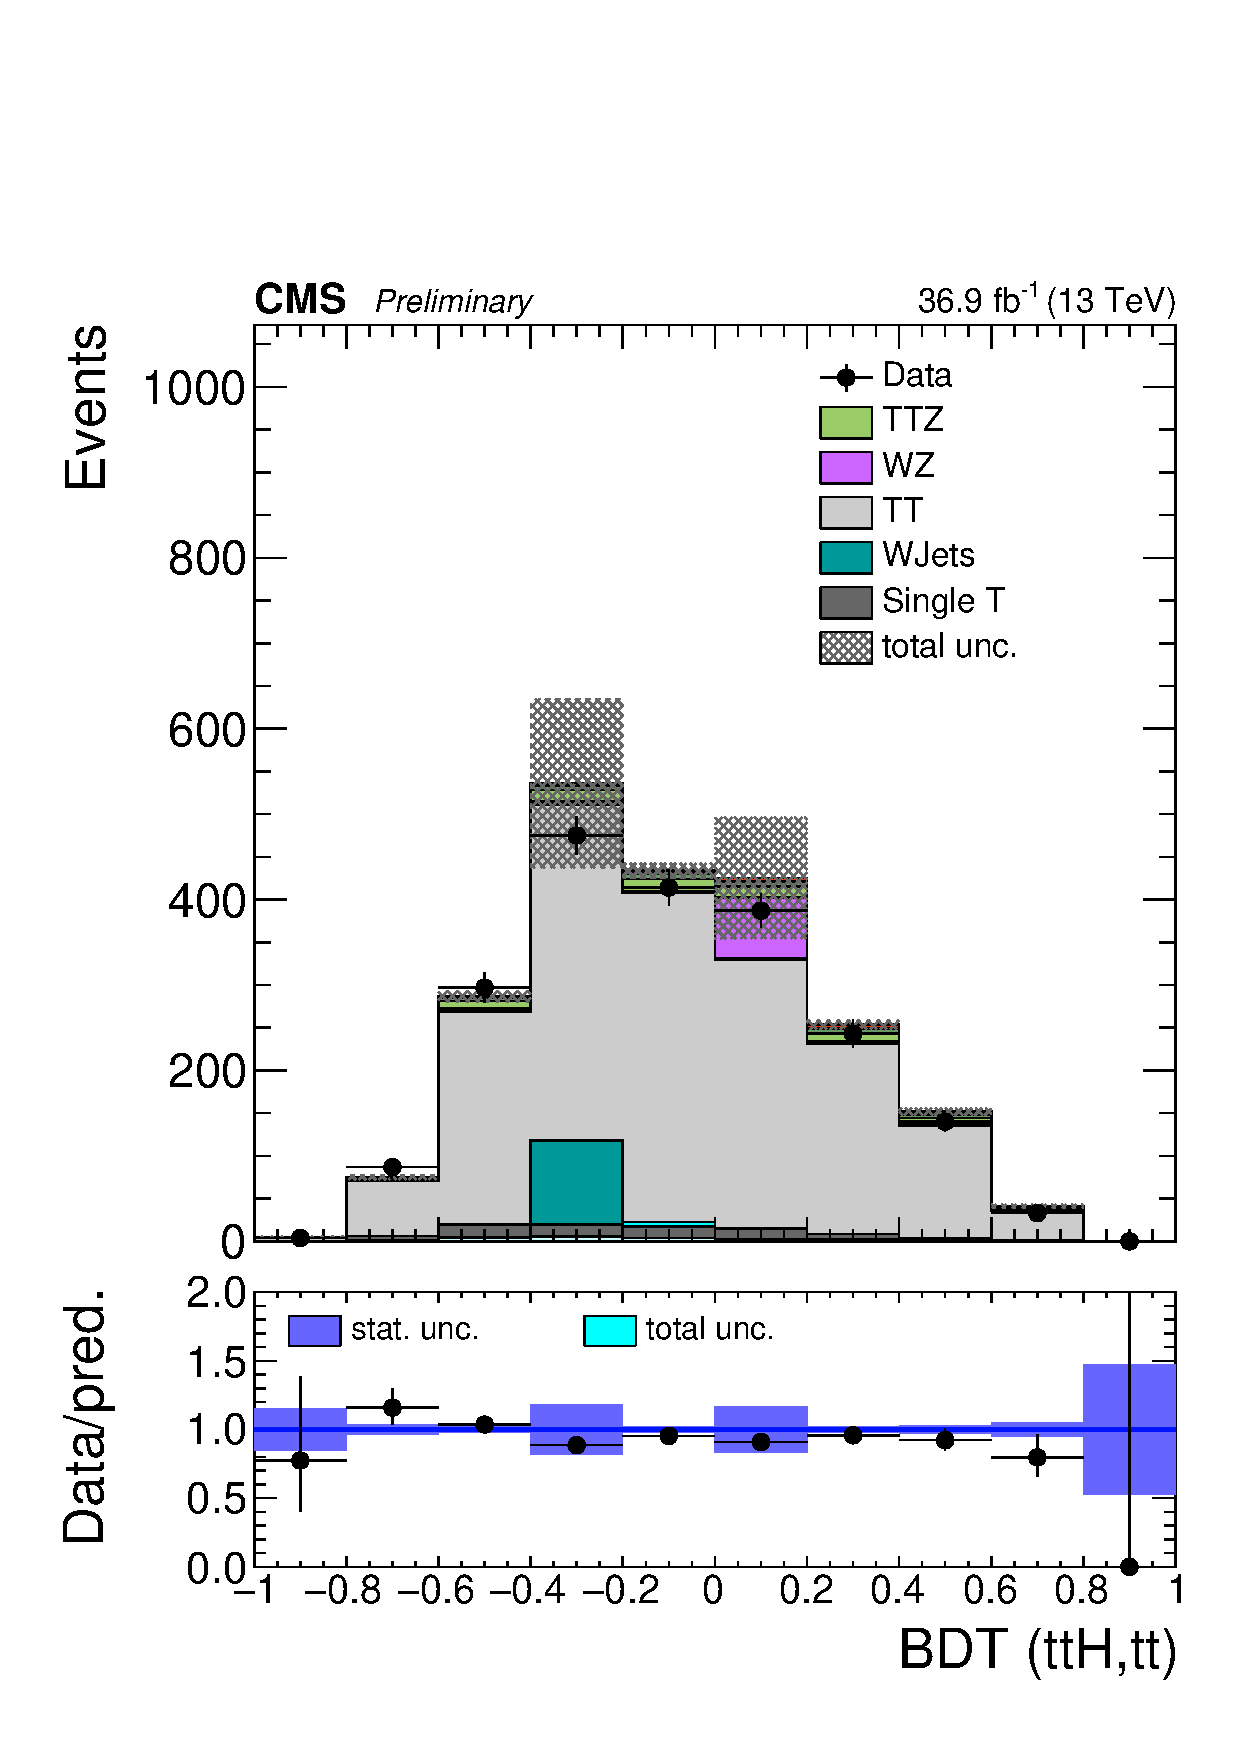
\includegraphics[width=0.30\linewidth]{plots_controlregions/2lss_appl_1fo_data/kinMVA_2lss_ttbar.pdf}
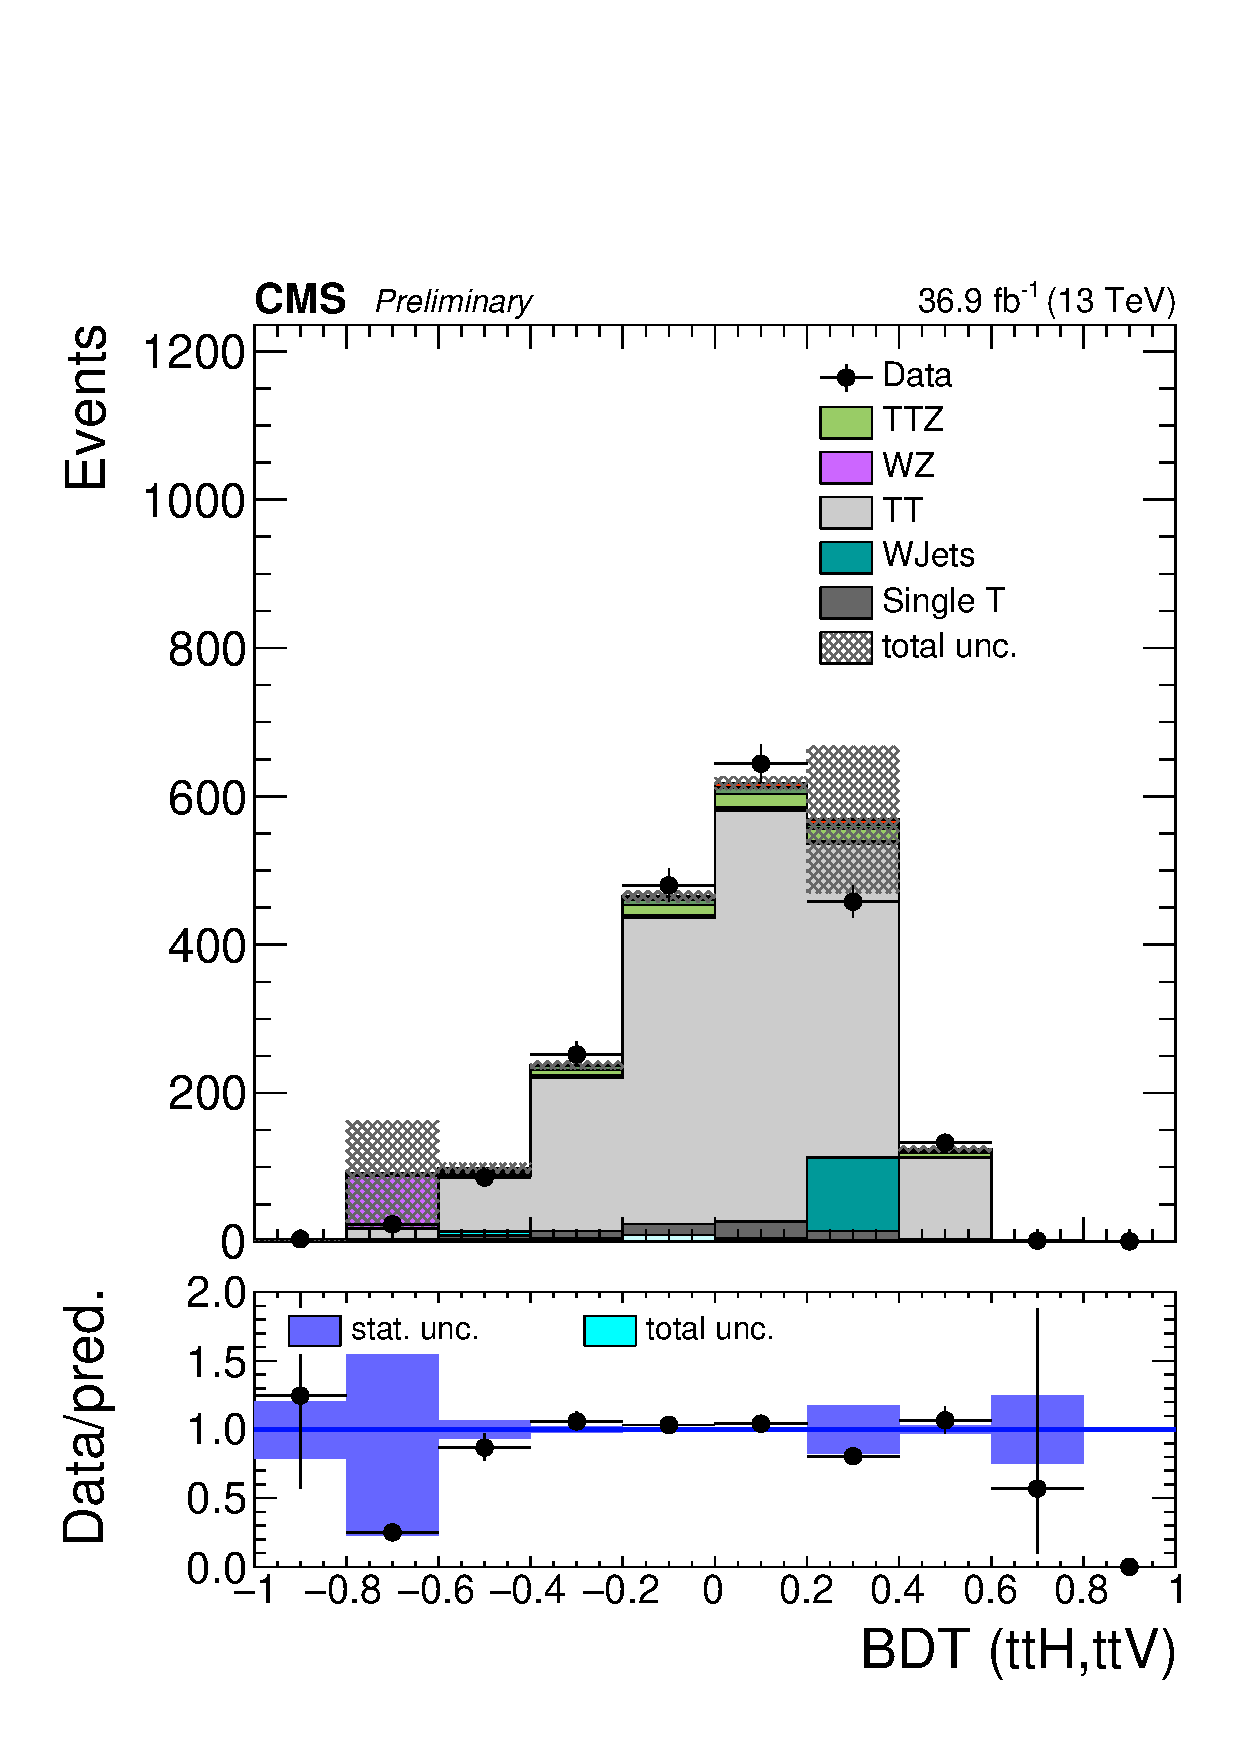
\includegraphics[width=0.30\linewidth]{plots_controlregions/2lss_appl_1fo_data/kinMVA_2lss_ttV.pdf}
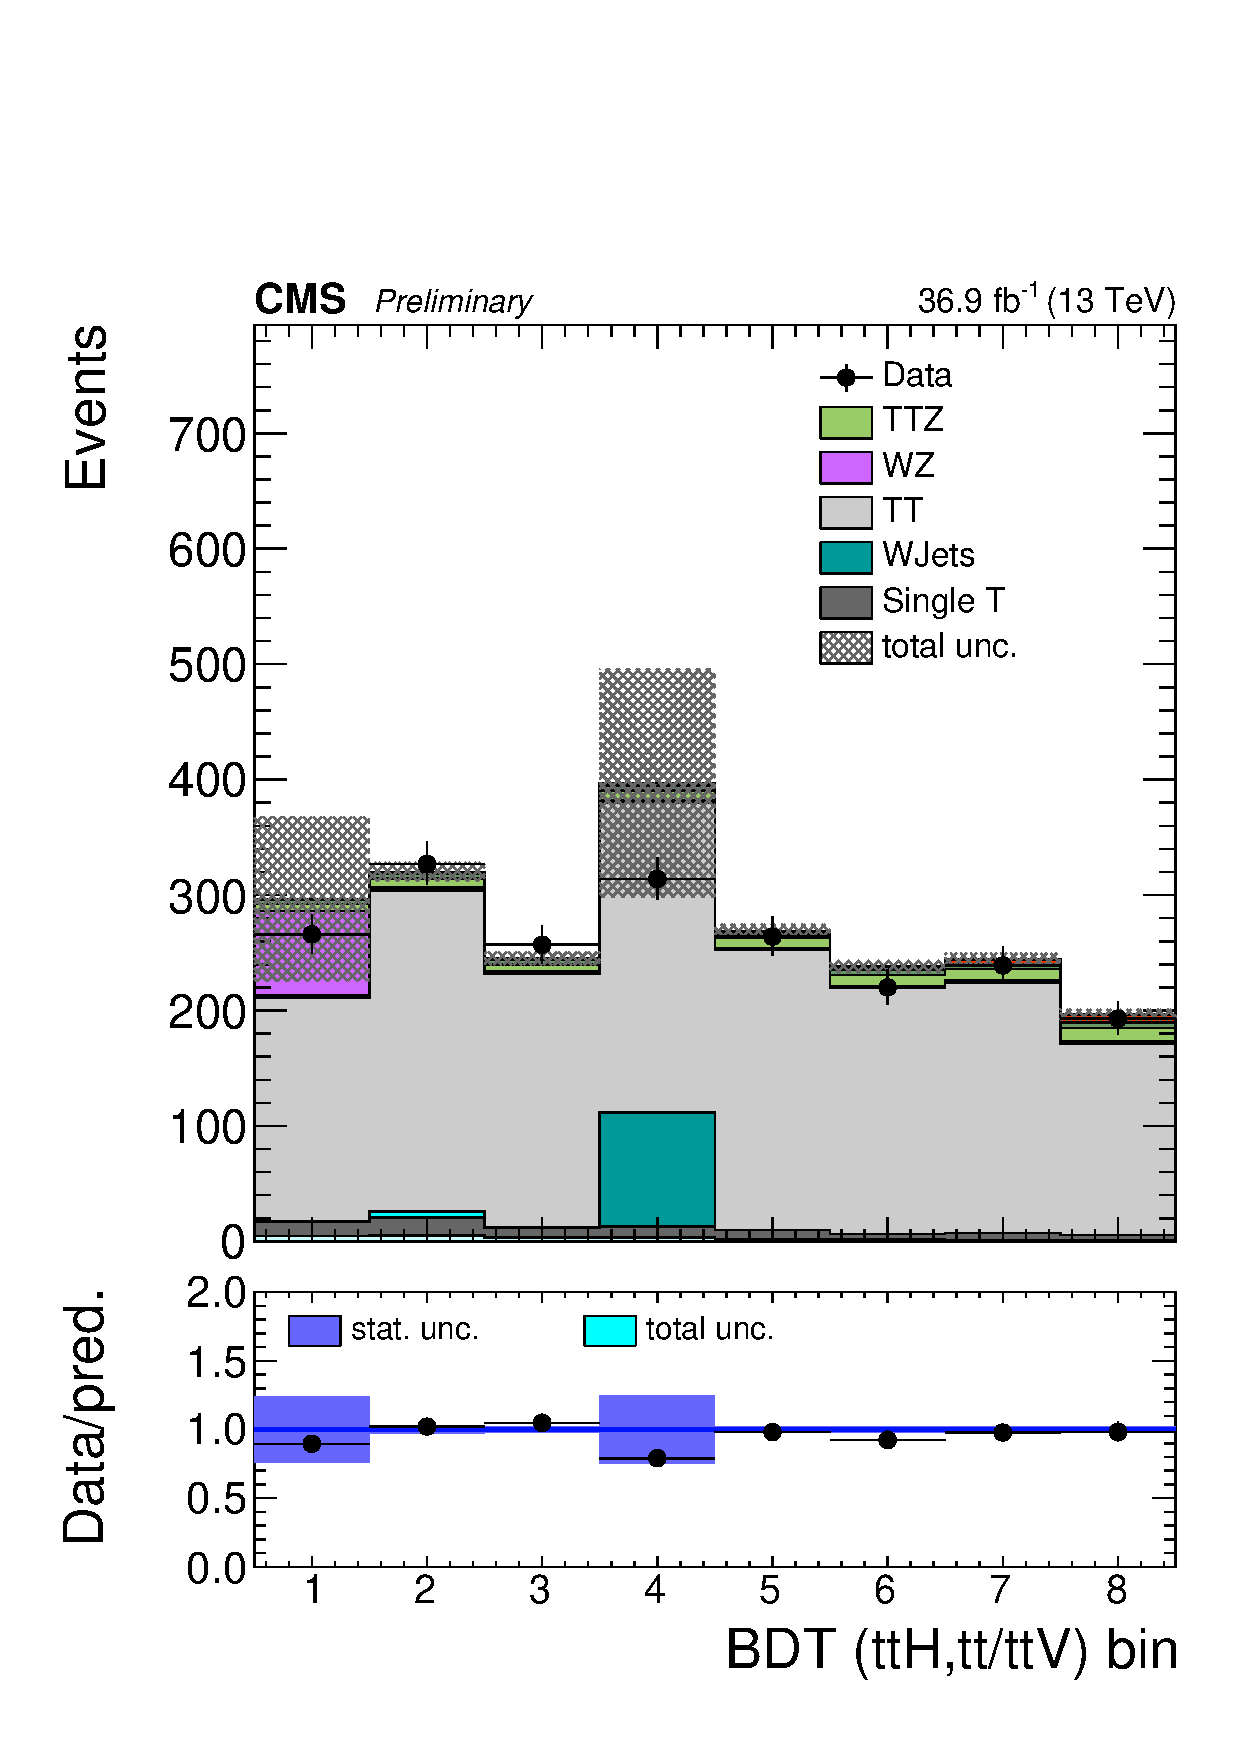
\includegraphics[width=0.30\linewidth]{plots_controlregions/2lss_appl_1fo_data/kinMVA_2lss_bins8_withBDTv8_withHj_ourBinning.pdf}
\caption{Data and simulation distributions in the 2lss control region with exactly one fakeable lepton failing the tight selection requirements.
From top left to bottom right: the cone-corrected $\pt$ of the failing lepton, the flavor of the lepton pair, the signal BDT discriminators against $\ttbar$ and ttV including the 2D-binned version as described in Section~\ref{sec:extraction}.
Uncertainties are statistical only.
}
\label{fig:cr_2lss_appl_1fo_1}
\end{figure}

\begin{figure}[!htb]
\centering
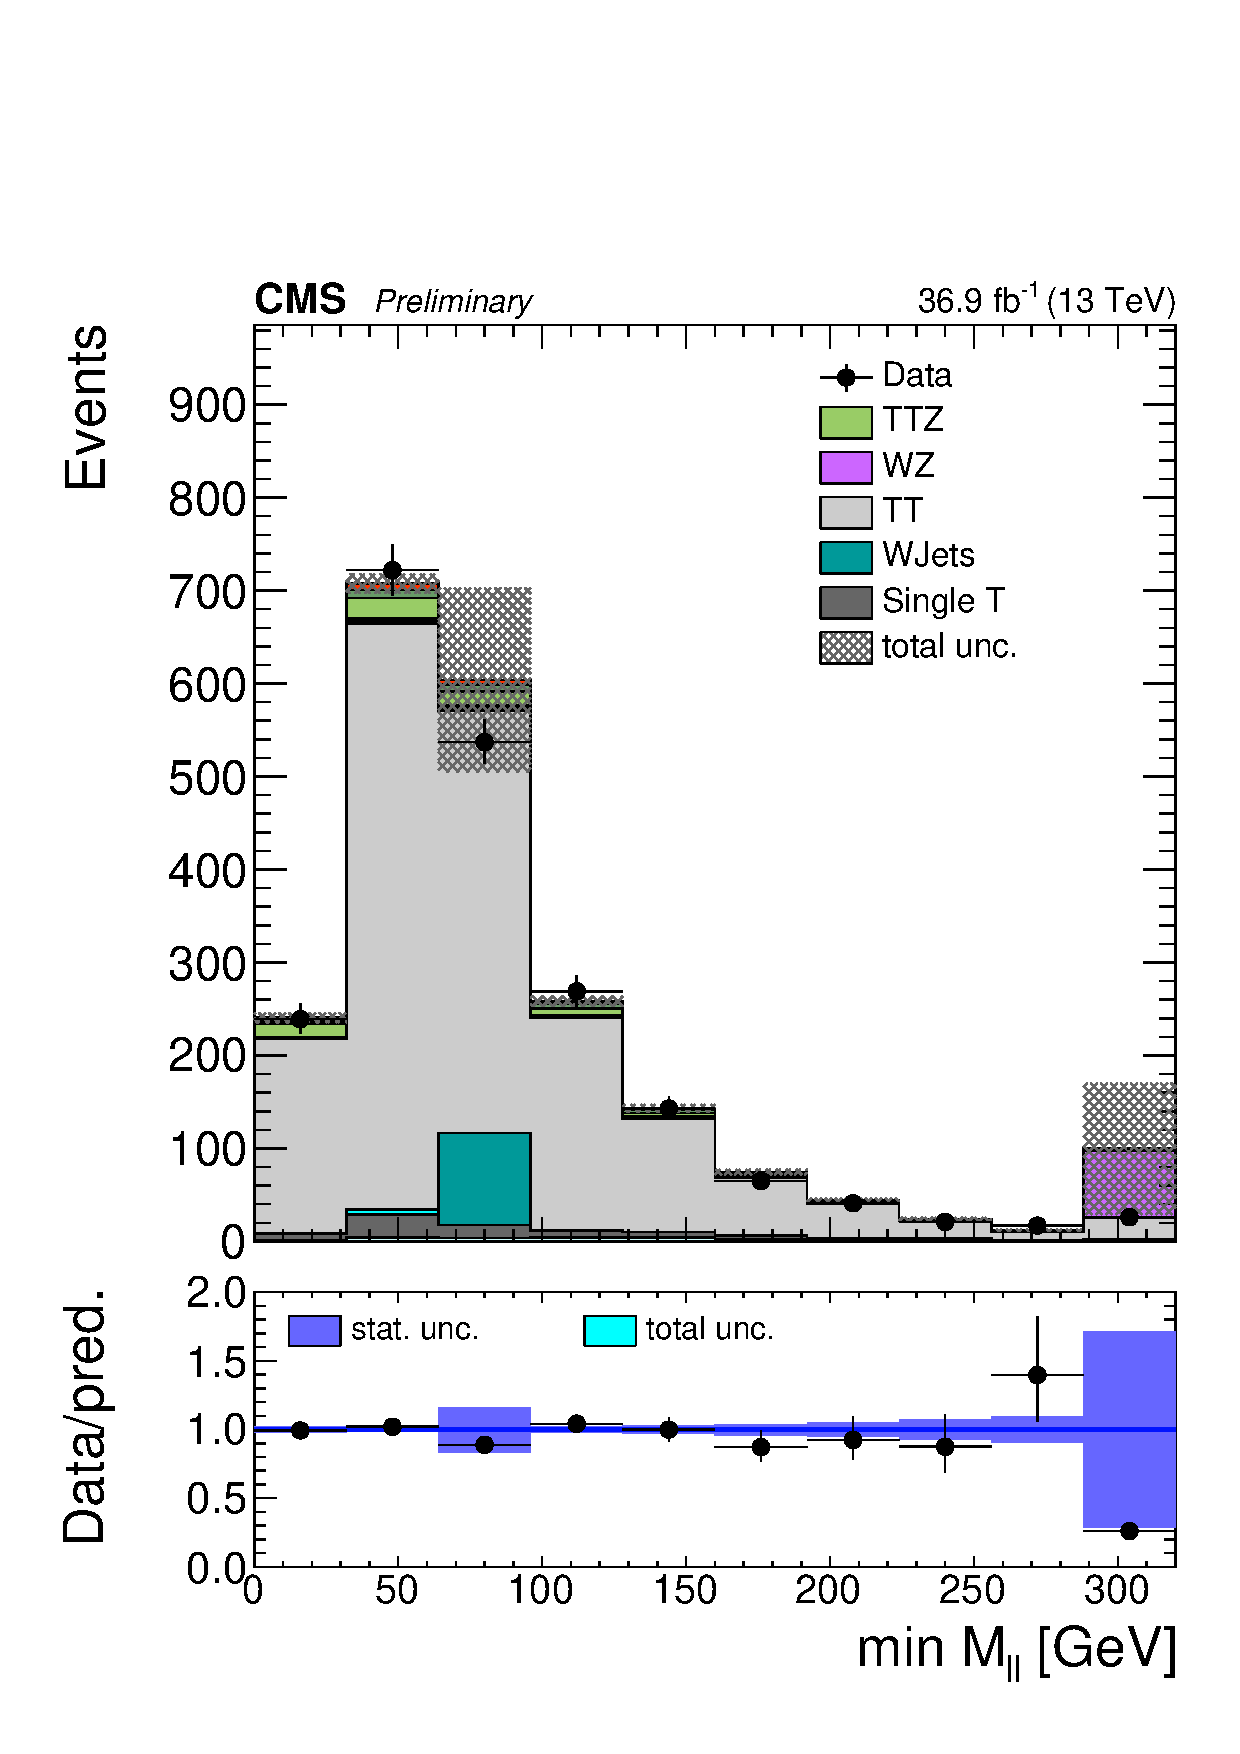
\includegraphics[width=0.30\linewidth]{plots_controlregions/2lss_appl_1fo_data/minMllAFAS.pdf}
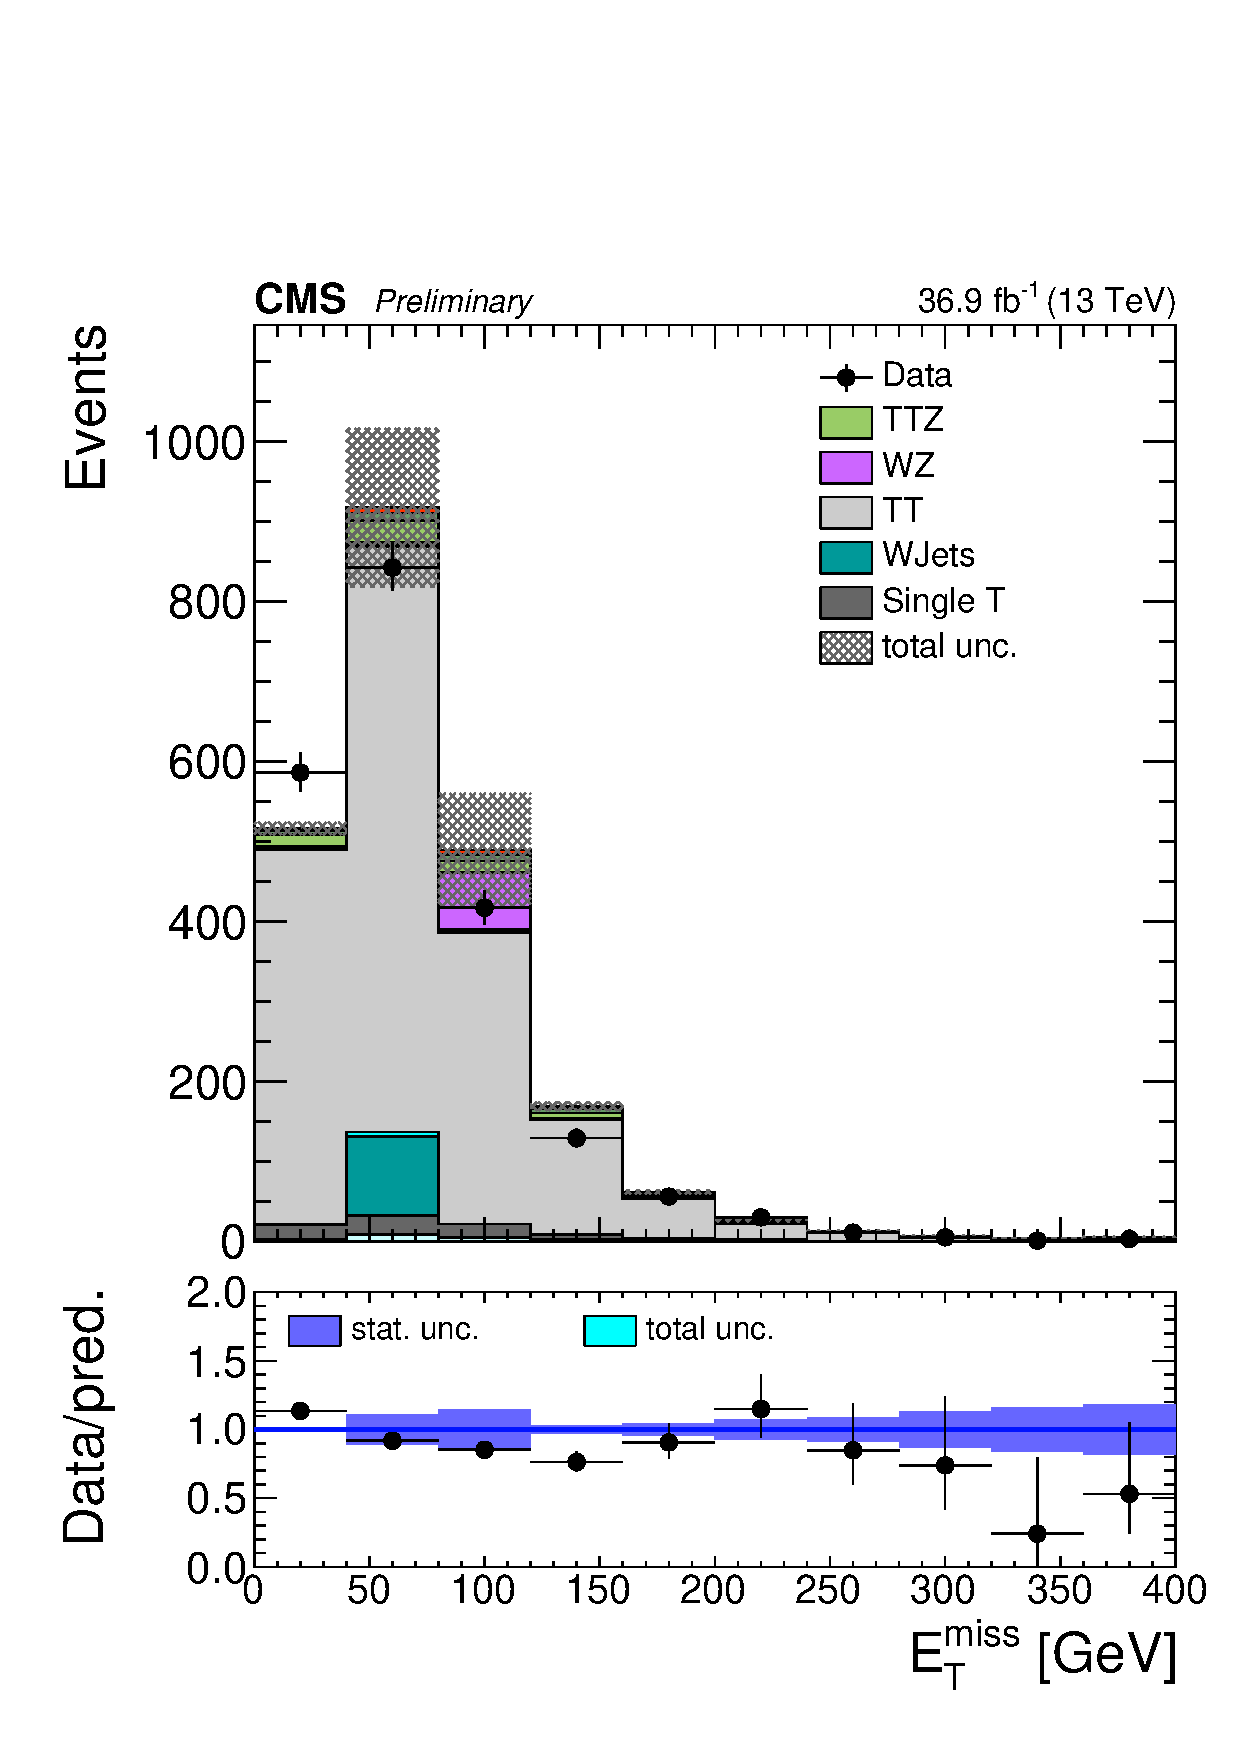
\includegraphics[width=0.30\linewidth]{plots_controlregions/2lss_appl_1fo_data/met.pdf}
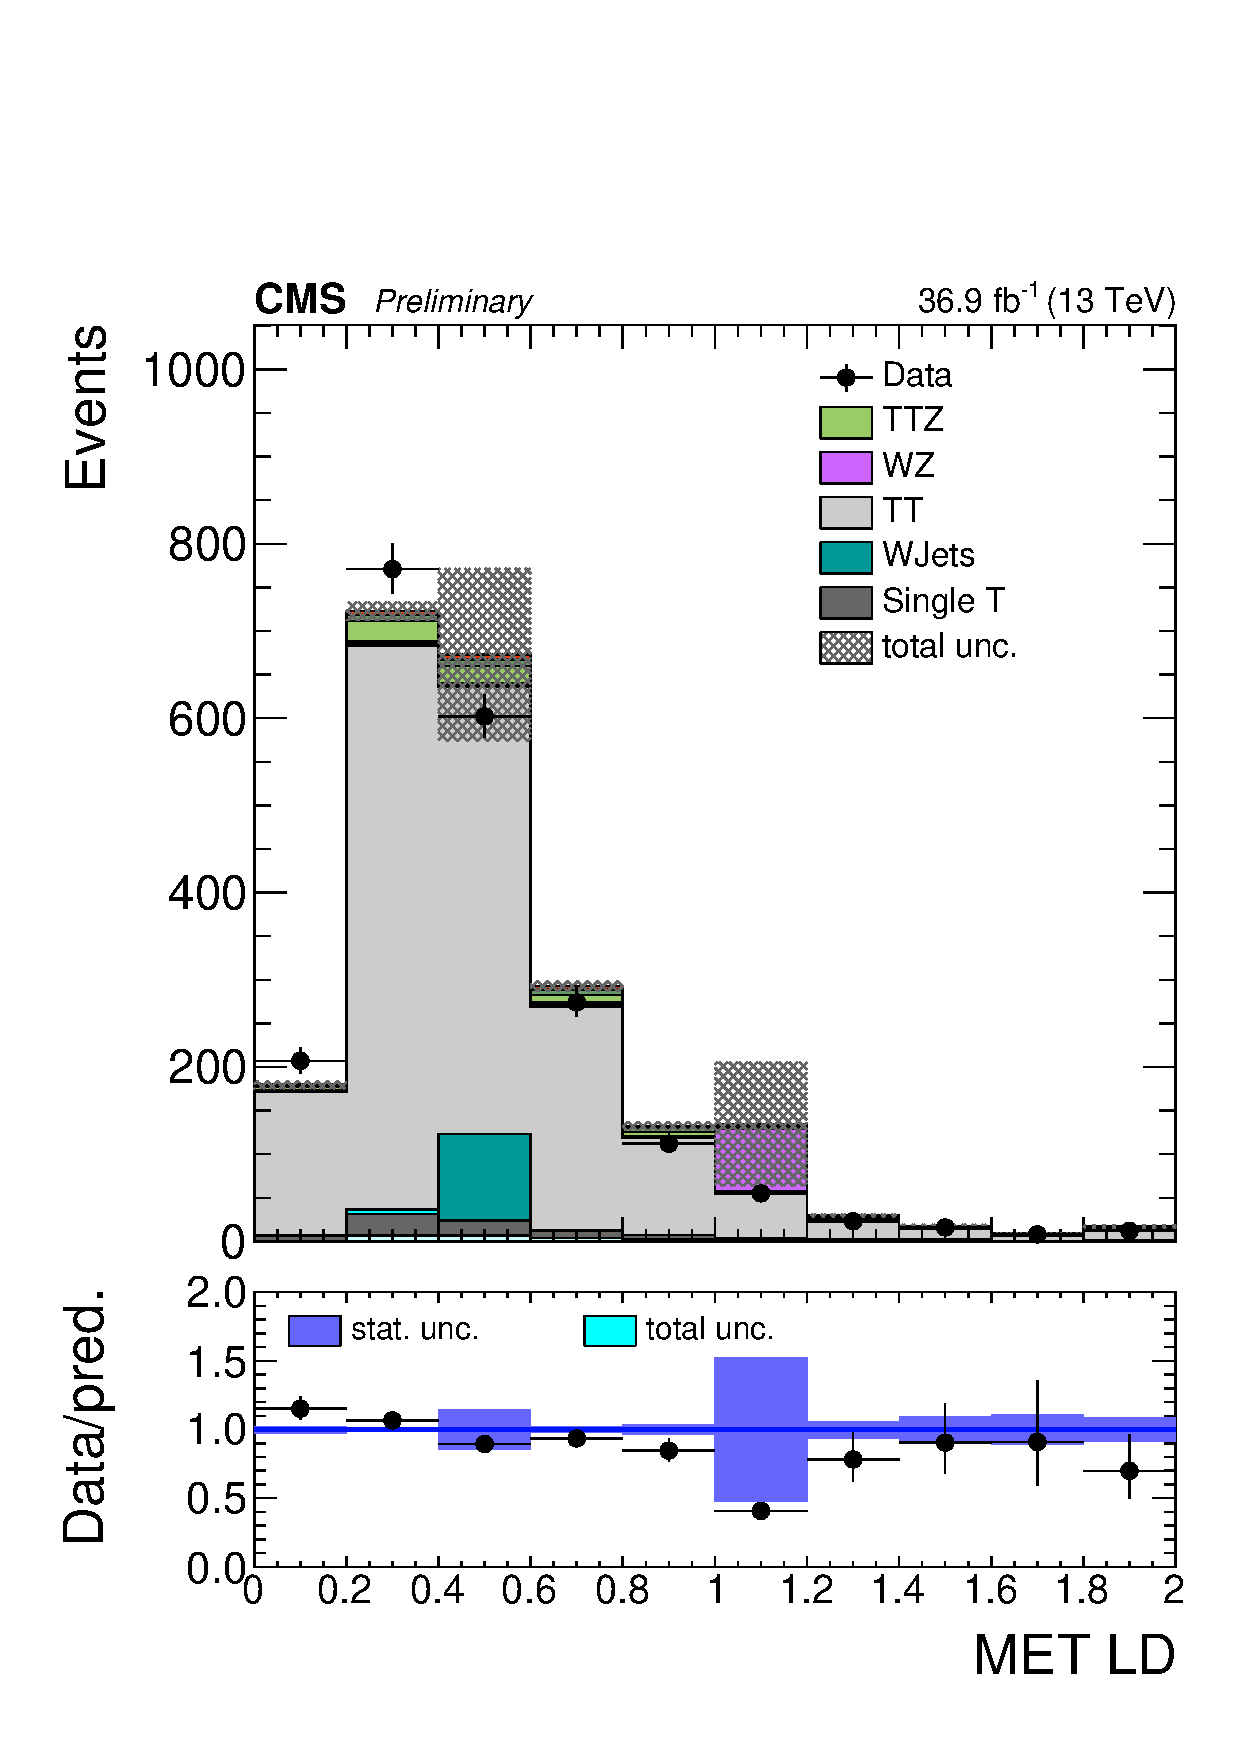
\includegraphics[width=0.30\linewidth]{plots_controlregions/2lss_appl_1fo_data/metLD.pdf}\\
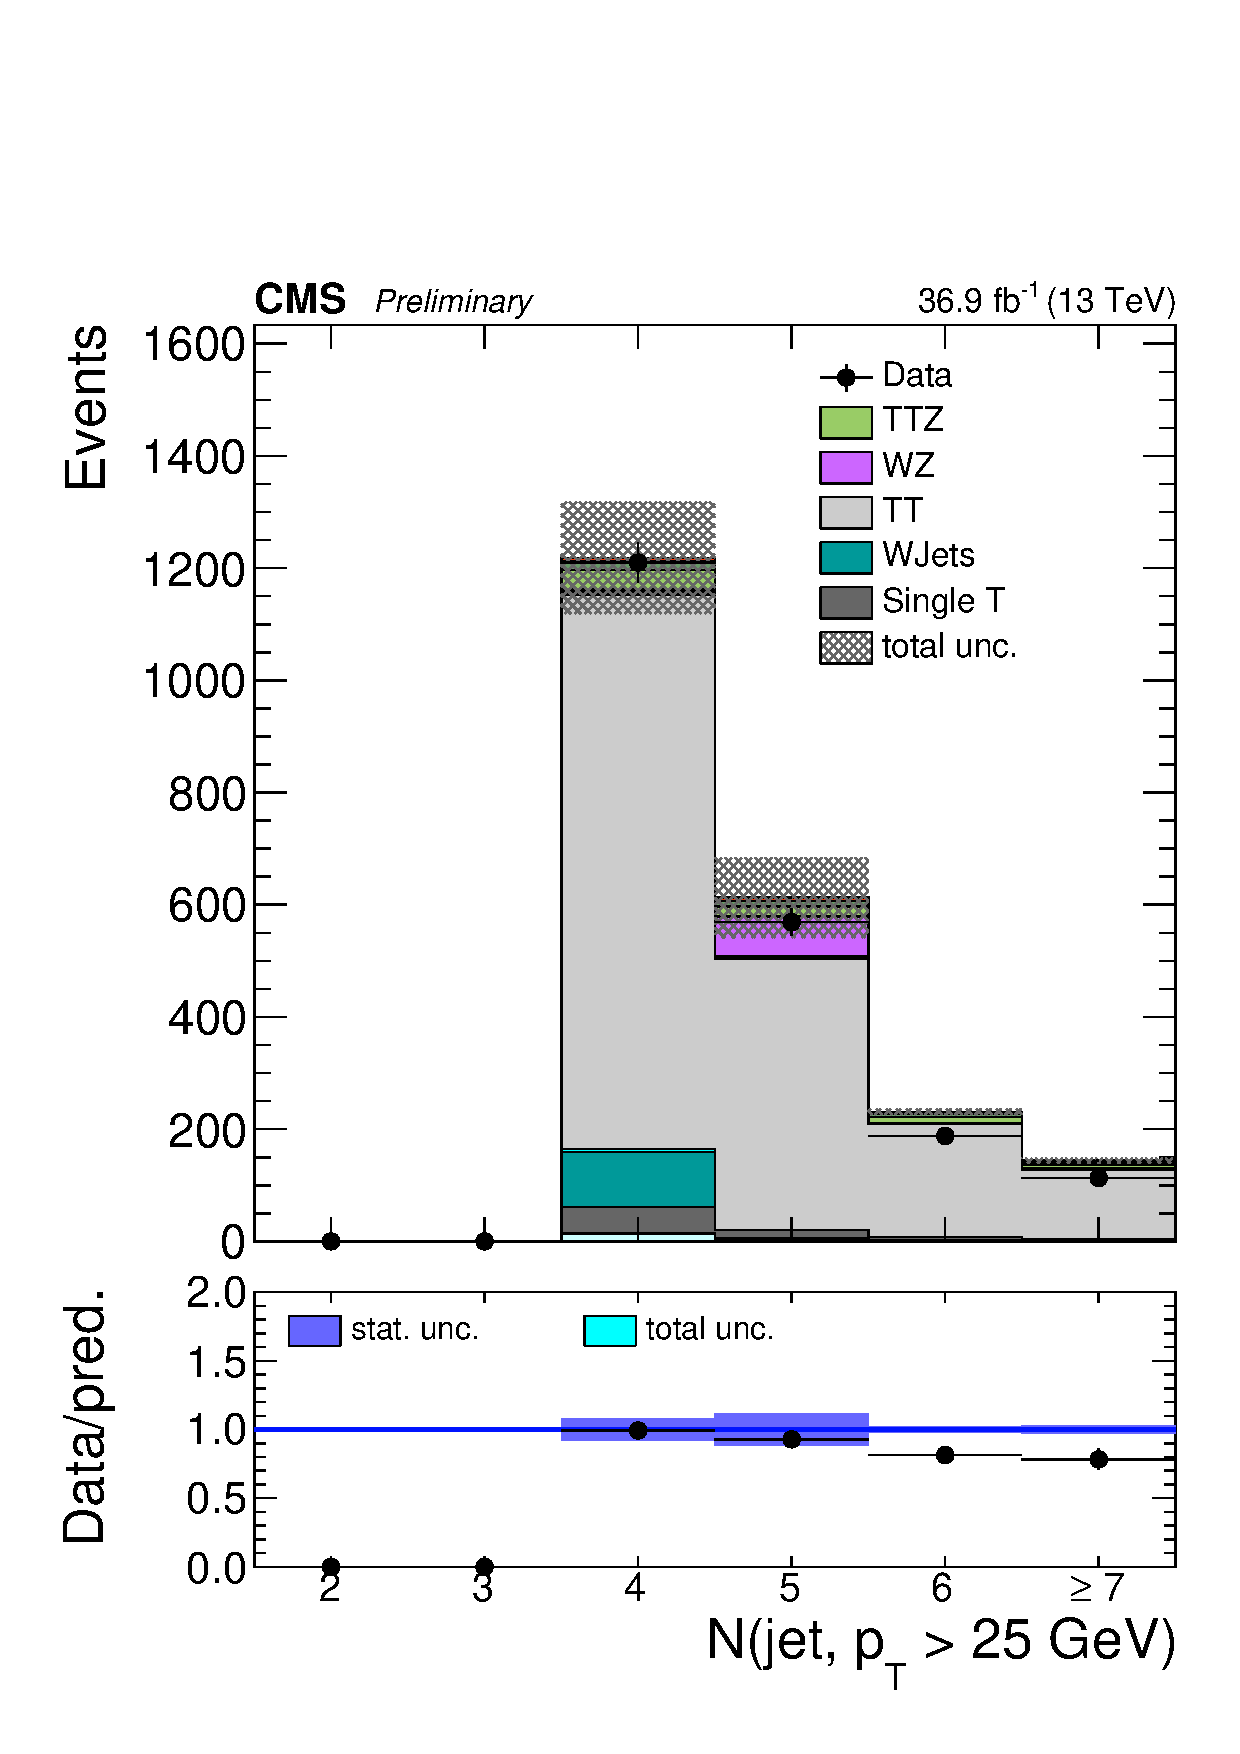
\includegraphics[width=0.30\linewidth]{plots_controlregions/2lss_appl_1fo_data/nJet25.pdf}
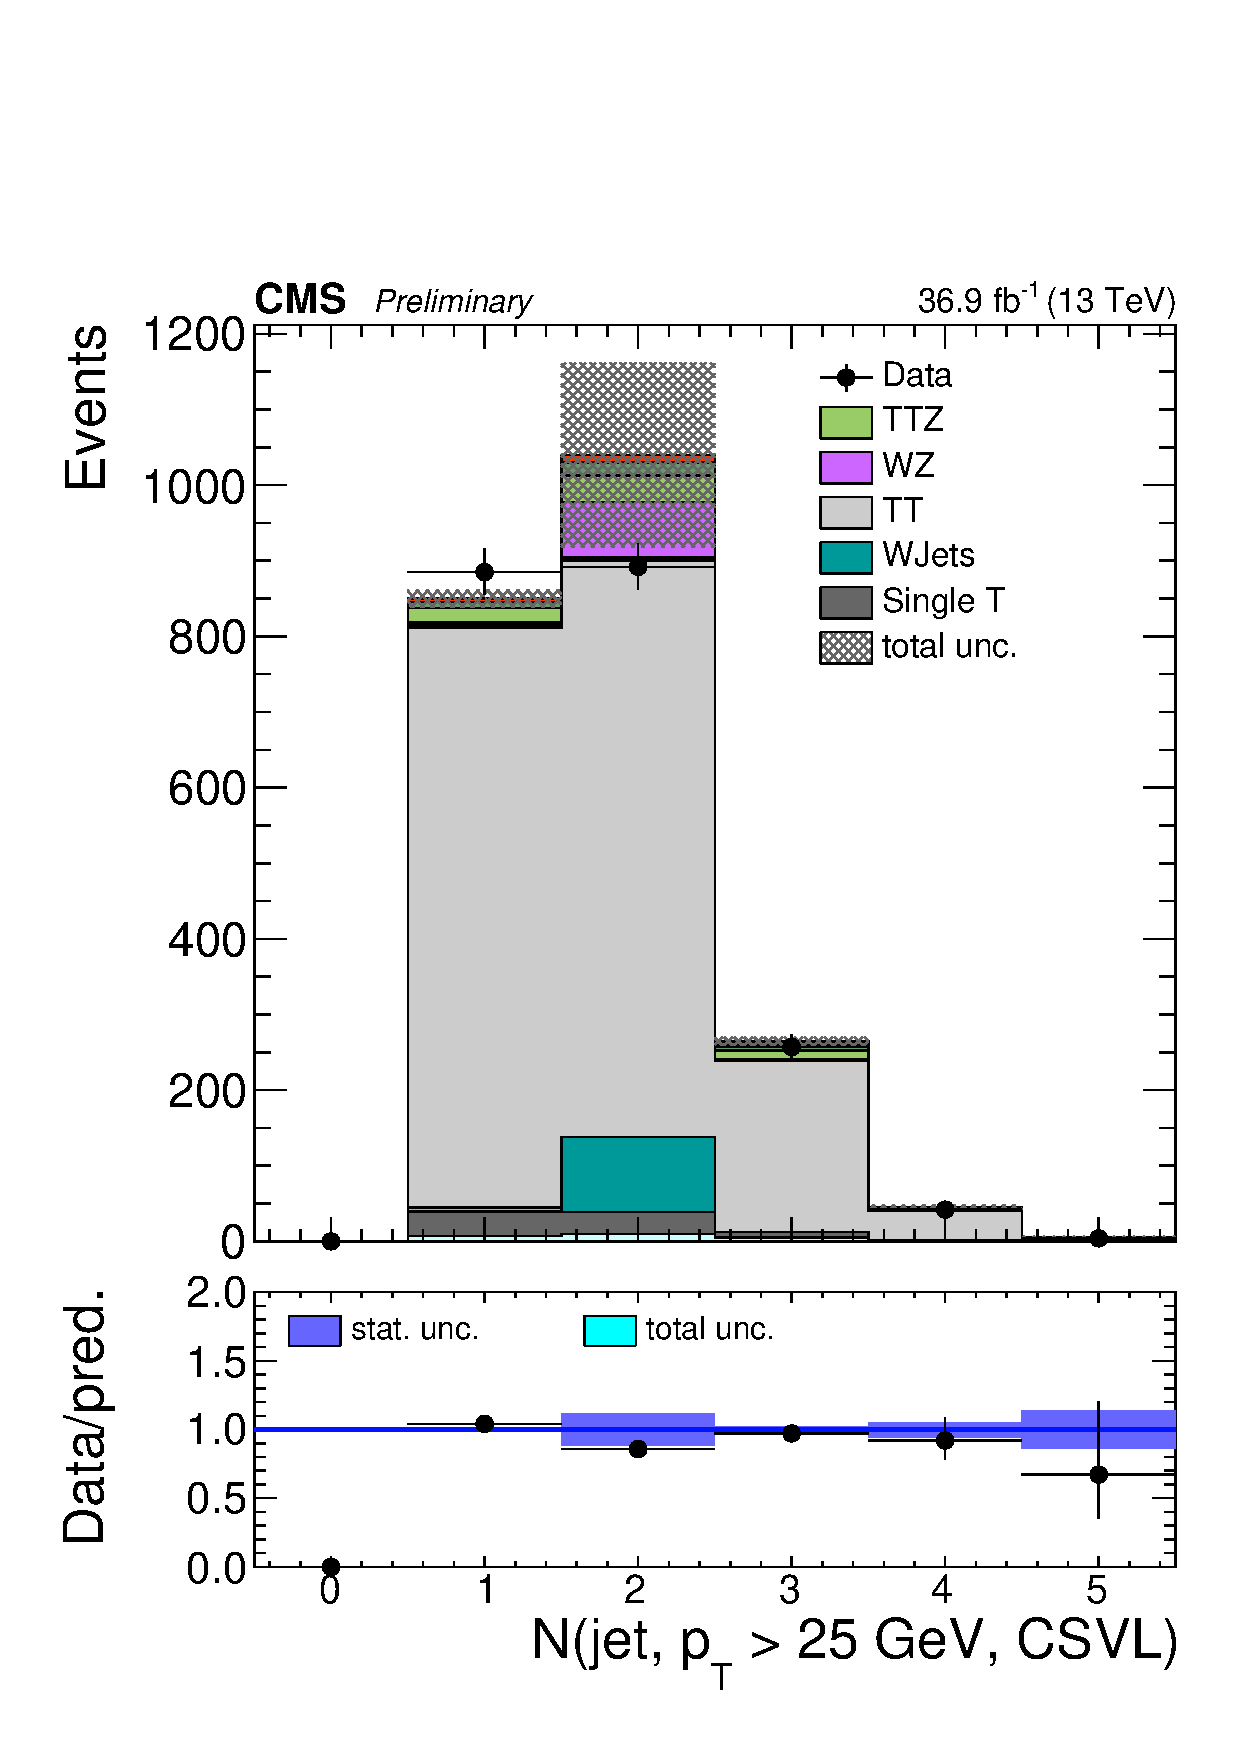
\includegraphics[width=0.30\linewidth]{plots_controlregions/2lss_appl_1fo_data/nBJetLoose25.pdf}
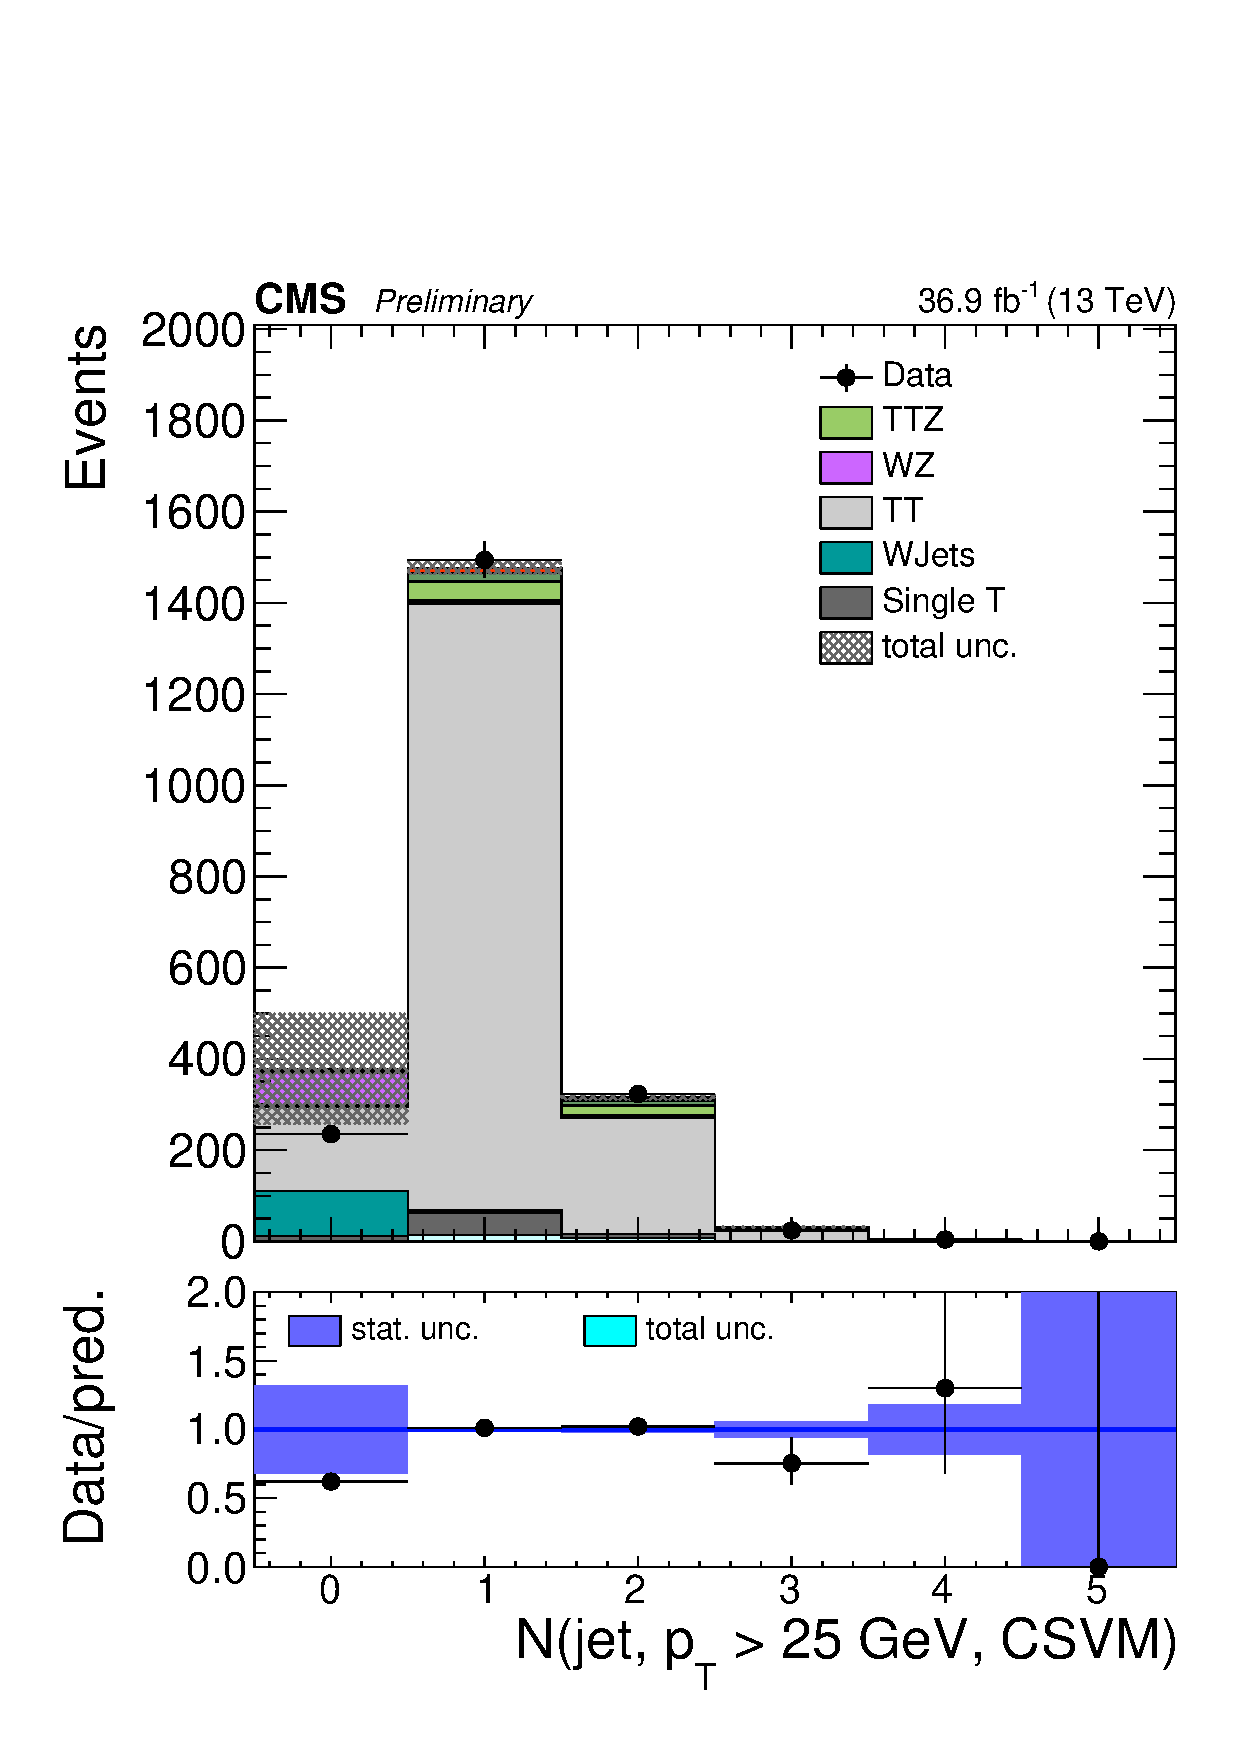
\includegraphics[width=0.30\linewidth]{plots_controlregions/2lss_appl_1fo_data/nBJetMedium25.pdf}\\
\caption{Data and simulation distributions in the 2lss control region with exactly one fakeable lepton failing the tight selection requirements.
From top left to bottom right: the minimum invariant mass of loose di-lepton pairs, $E_\mathrm{T}^\mathrm{miss}$, $E_\mathrm{T}^\mathrm{miss}LD$, multiplicity of inclusive and b-tagged jets.
cone-corrected $\pt$ of the failing lepton, the flavor of the lepton pair, the signal BDT discriminators against $\ttbar$ and ttV.
Uncertainties are statistical only.
}
\label{fig:cr_2lss_appl_1fo_2}
\end{figure}

\begin{figure}[!htb]
\centering
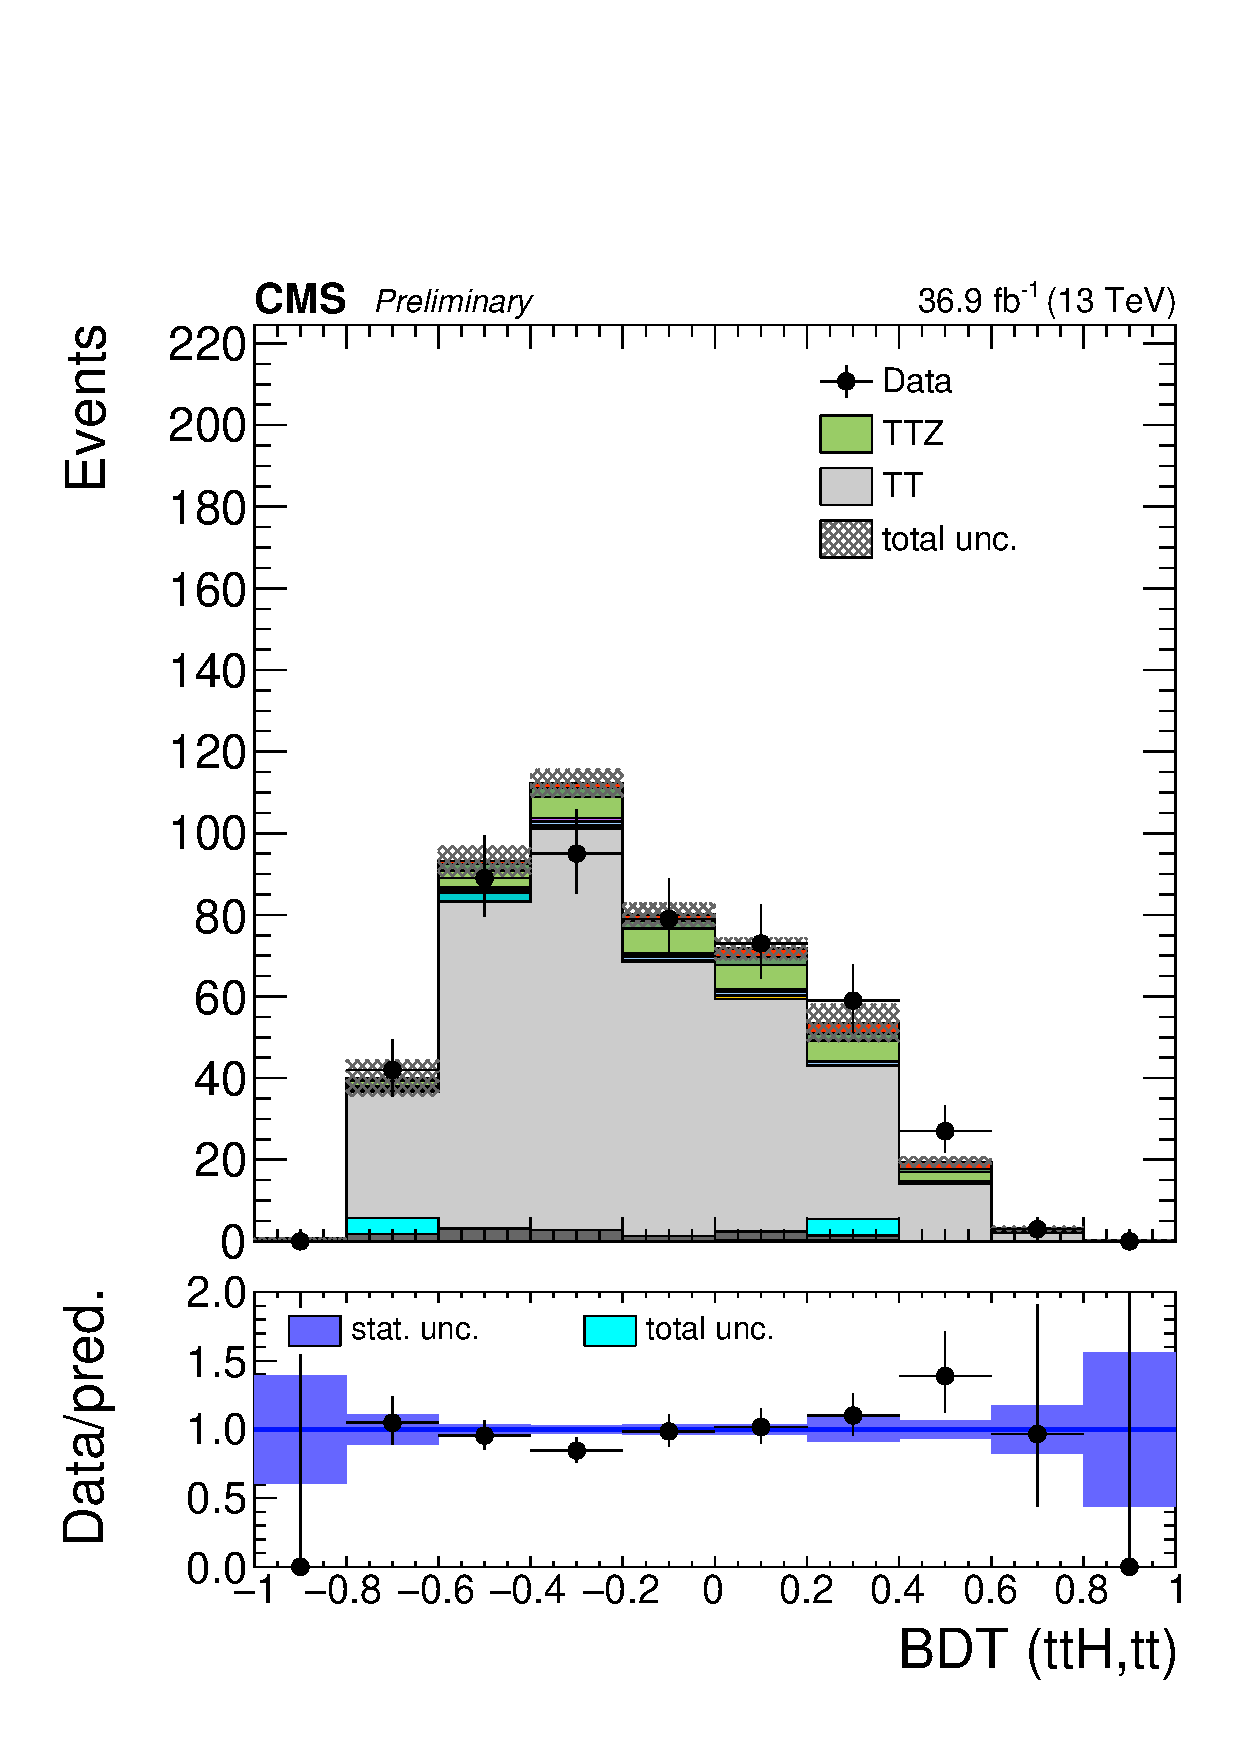
\includegraphics[width=0.30\linewidth]{plots_controlregions/3l_appl_1fo_data/kinMVA_3l_ttbar.pdf}
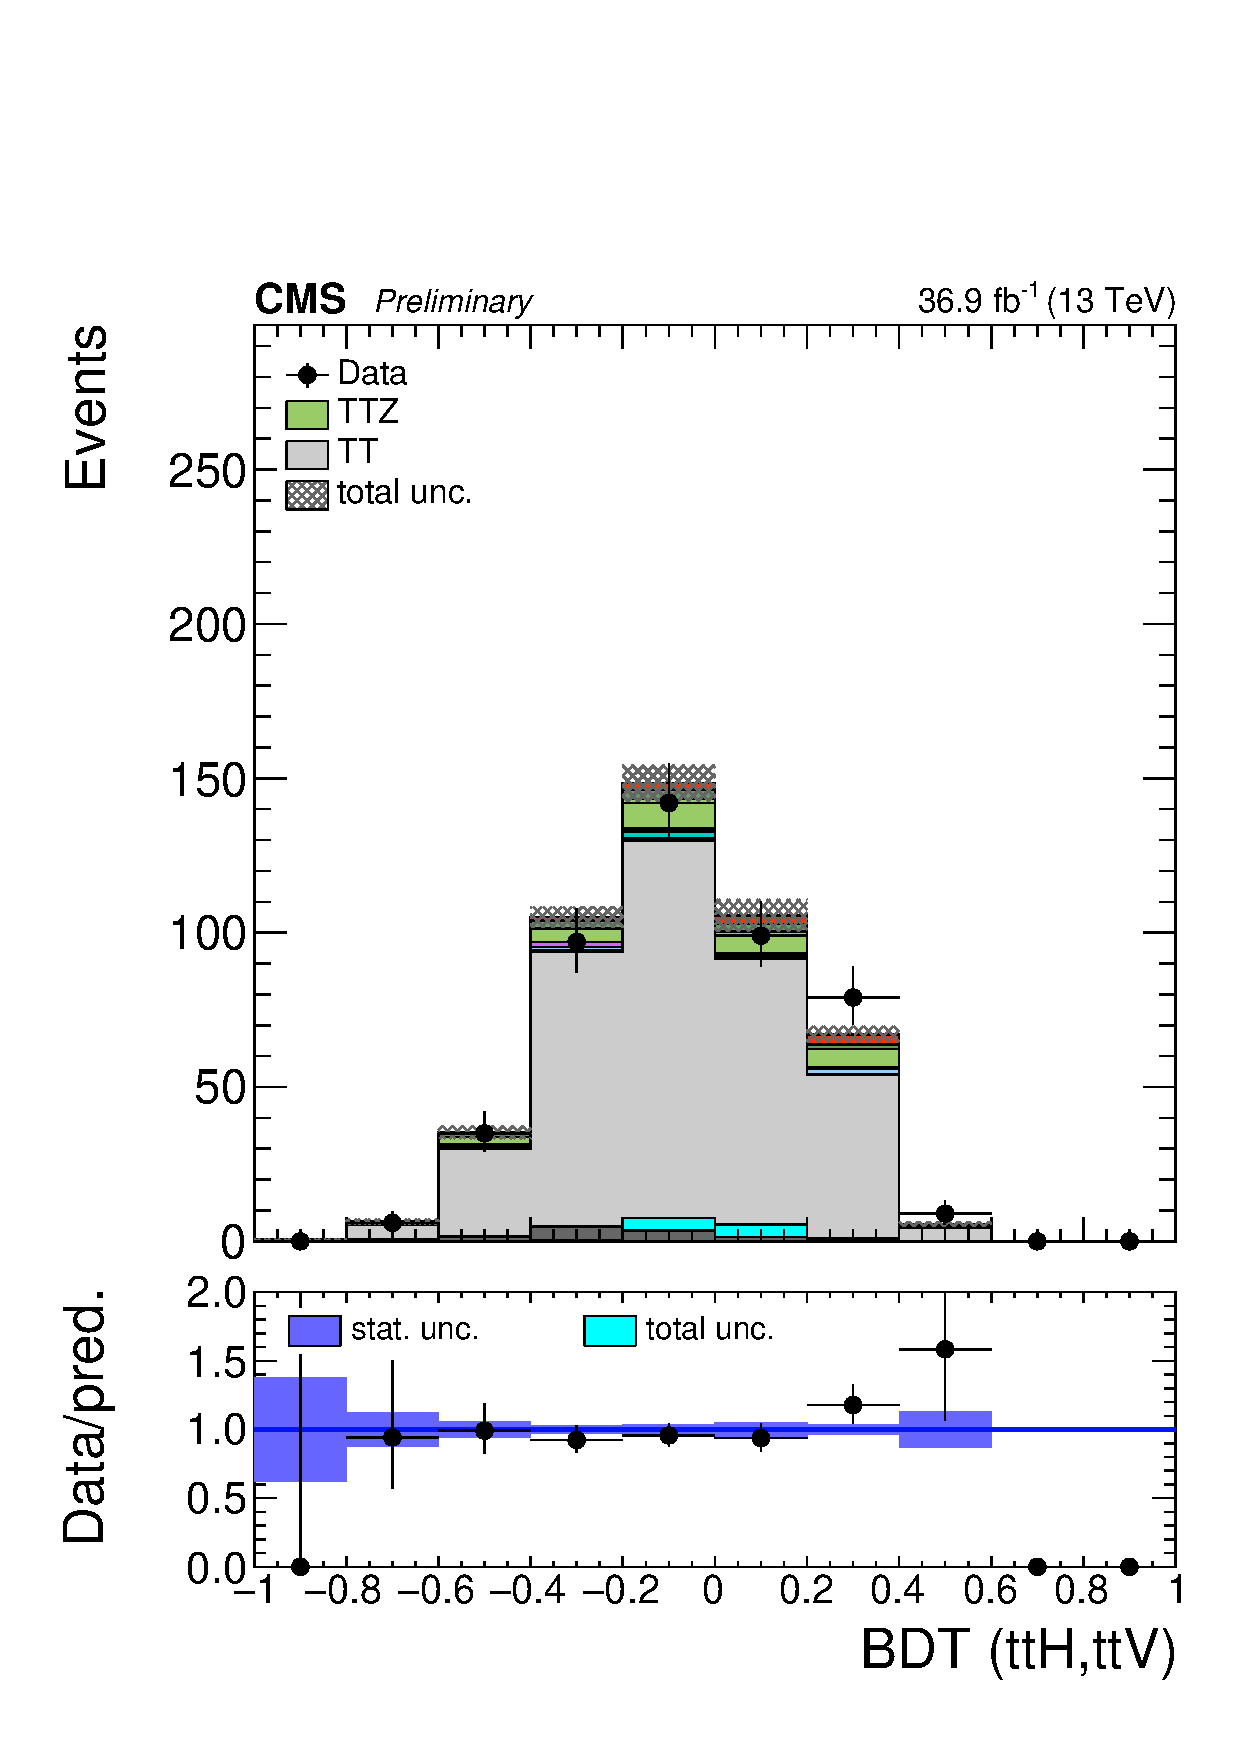
\includegraphics[width=0.30\linewidth]{plots_controlregions/3l_appl_1fo_data/kinMVA_3l_ttV.pdf}
%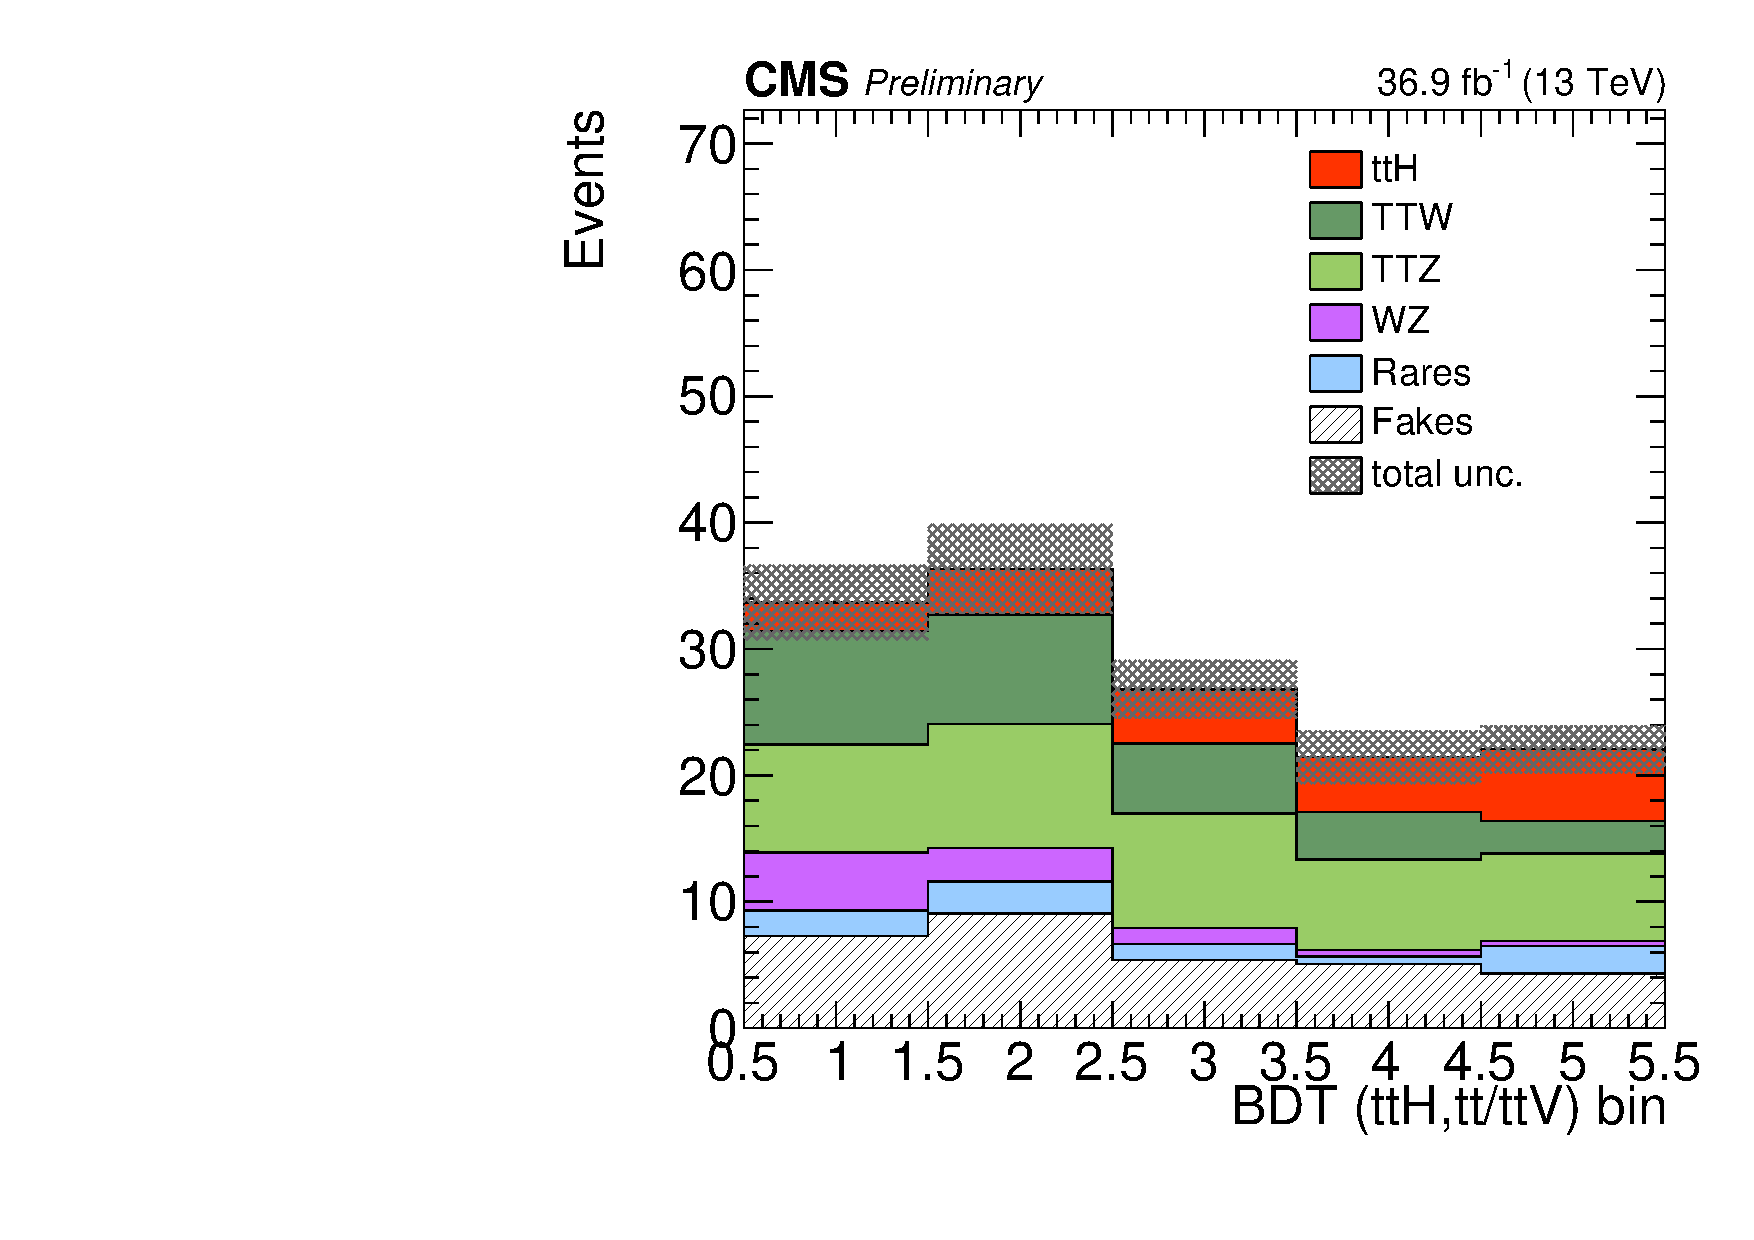
\includegraphics[width=0.30\linewidth]{plots_controlregions/3l_appl_1fo_data/kinMVA_3l_bins5_ourBinning.pdf}
\caption{Same as Fig.~\ref{fig:cr_2lss_appl_1fo_1}, for the 3l category of the analysis.}
\label{fig:cr_3l_appl_1fo_1}
\end{figure}


\begin{figure}[!htb]
\centering
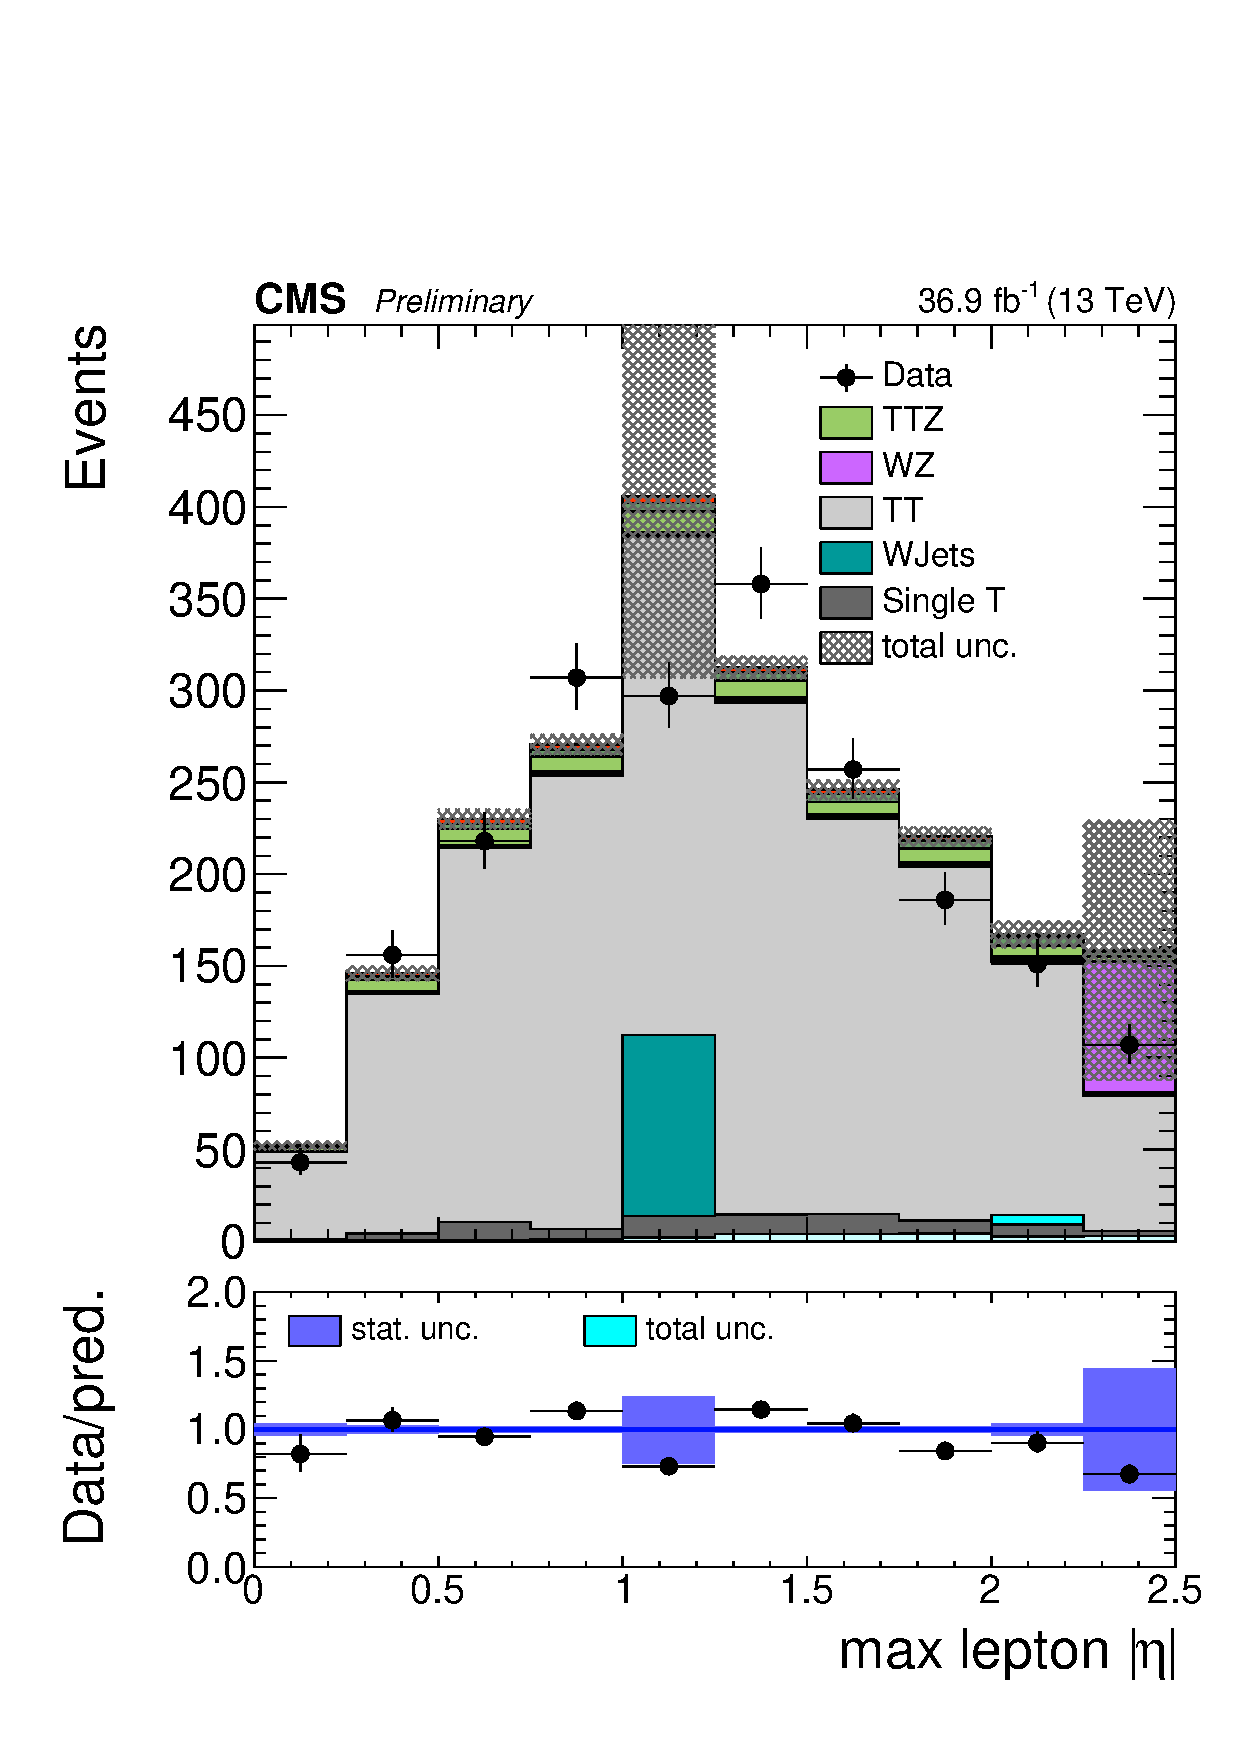
\includegraphics[width=0.30\linewidth]{plots_controlregions/2lss_appl_1fo_data/kinMVA_input_max_Lep_eta.pdf}
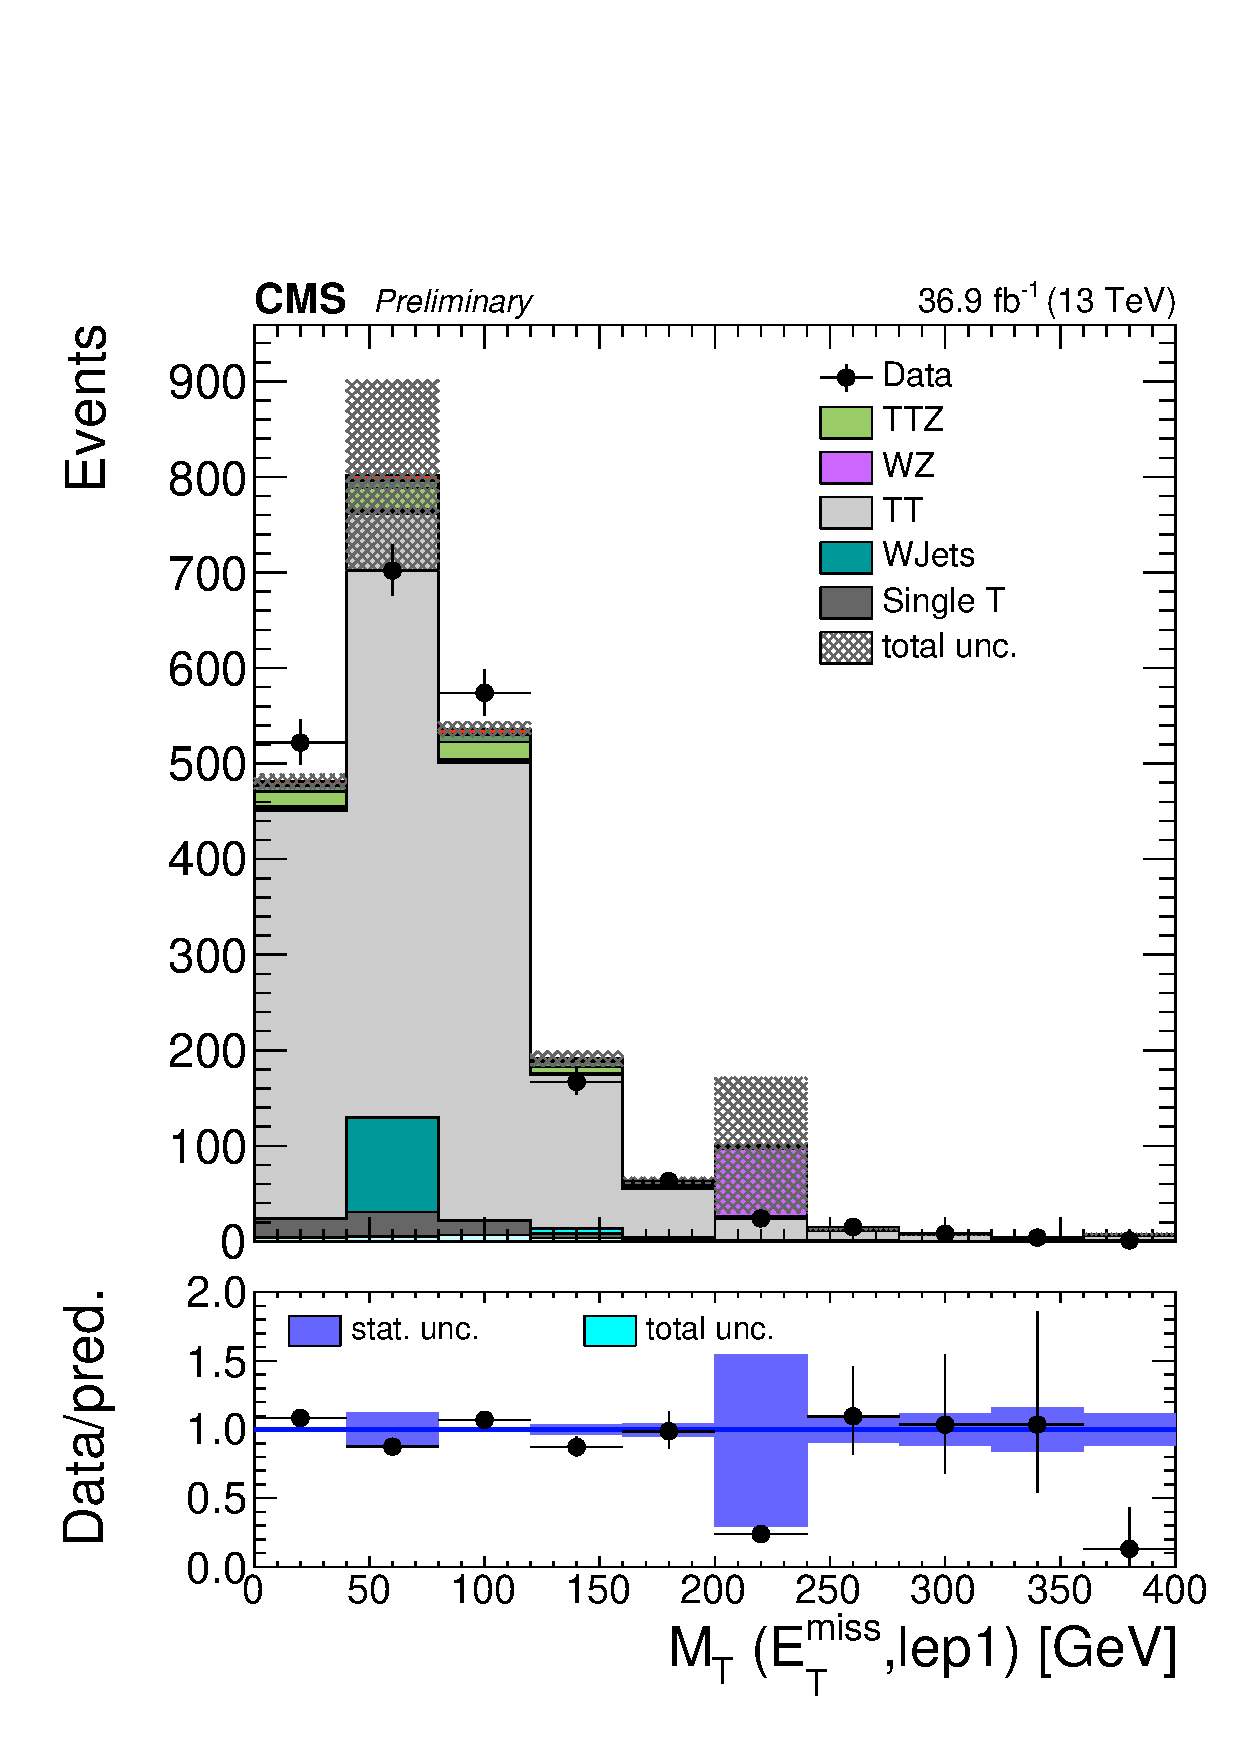
\includegraphics[width=0.30\linewidth]{plots_controlregions/2lss_appl_1fo_data/kinMVA_input_MT_met_lep1.pdf}
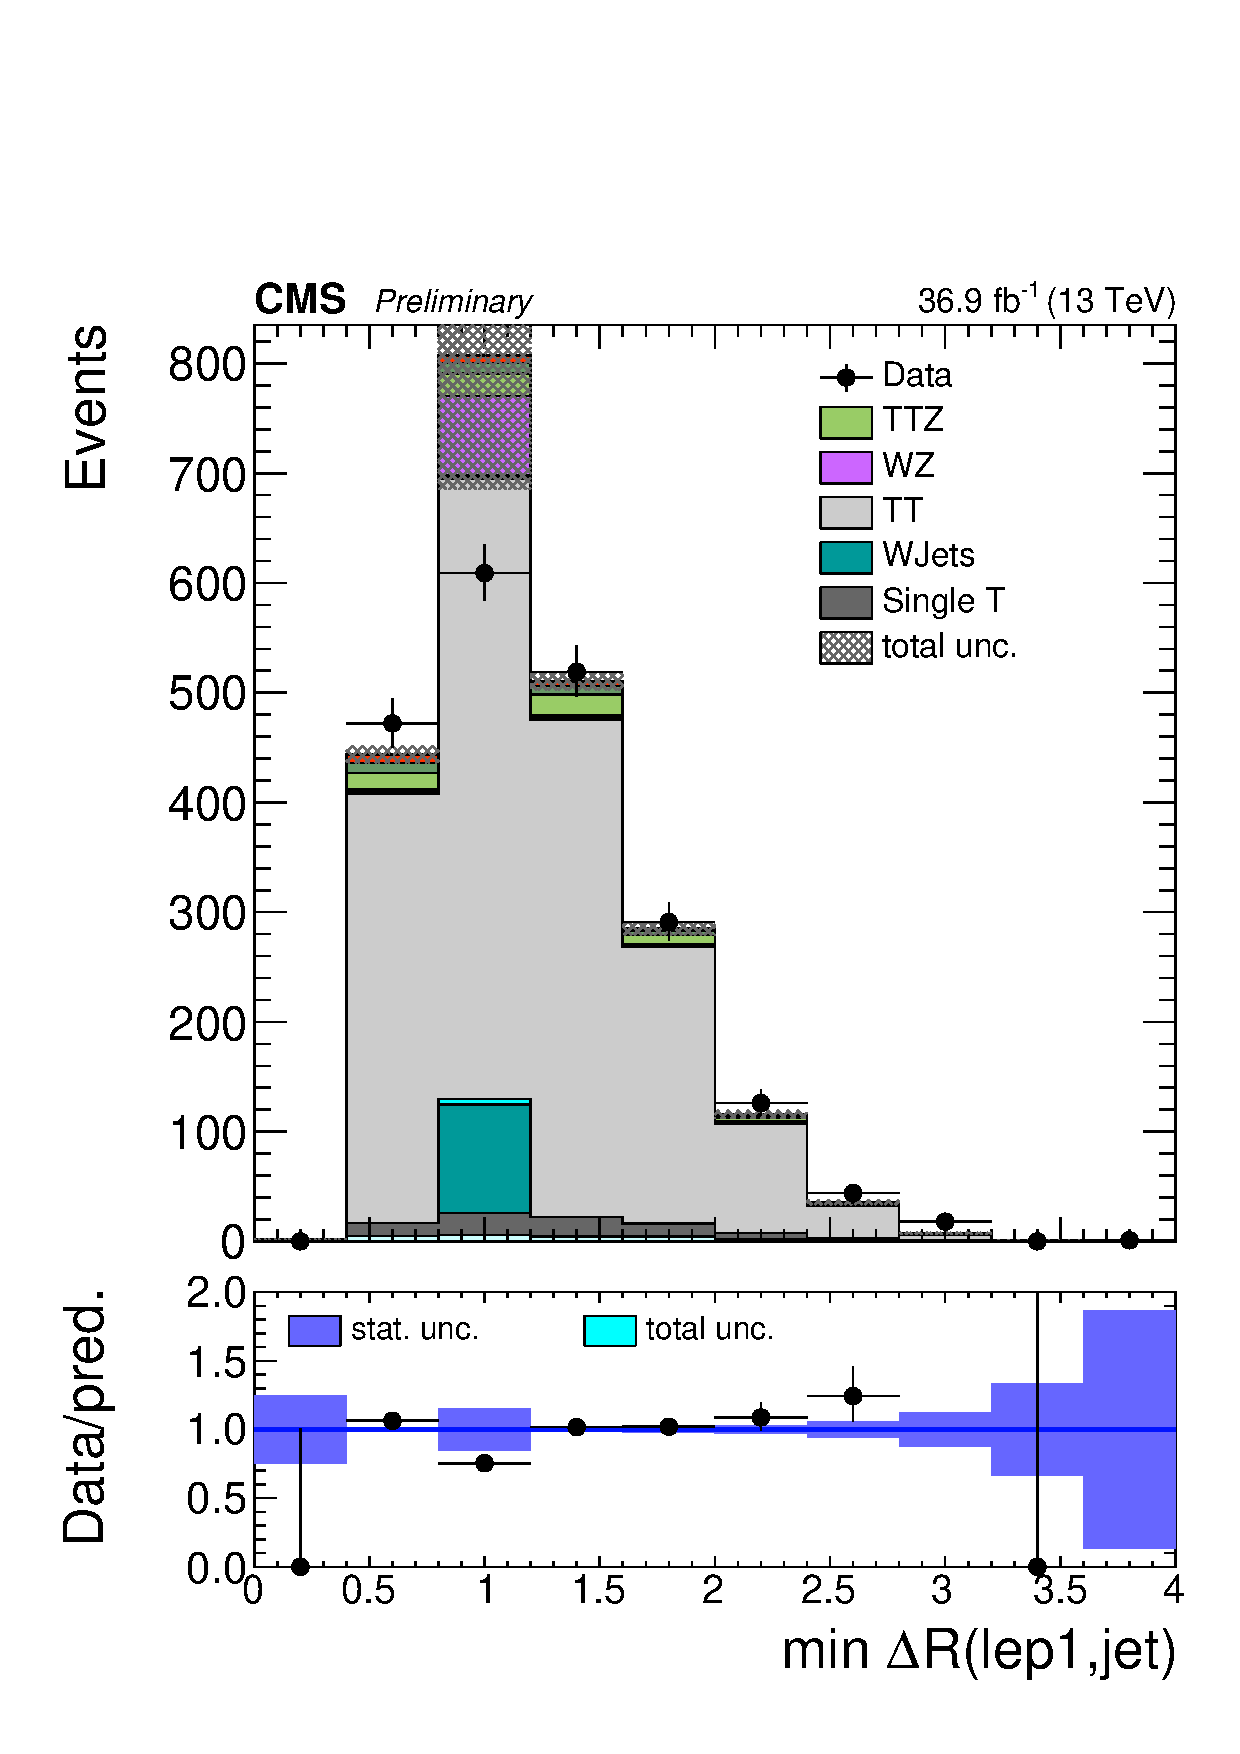
\includegraphics[width=0.30\linewidth]{plots_controlregions/2lss_appl_1fo_data/kinMVA_input_mindr_lep1_jet.pdf}
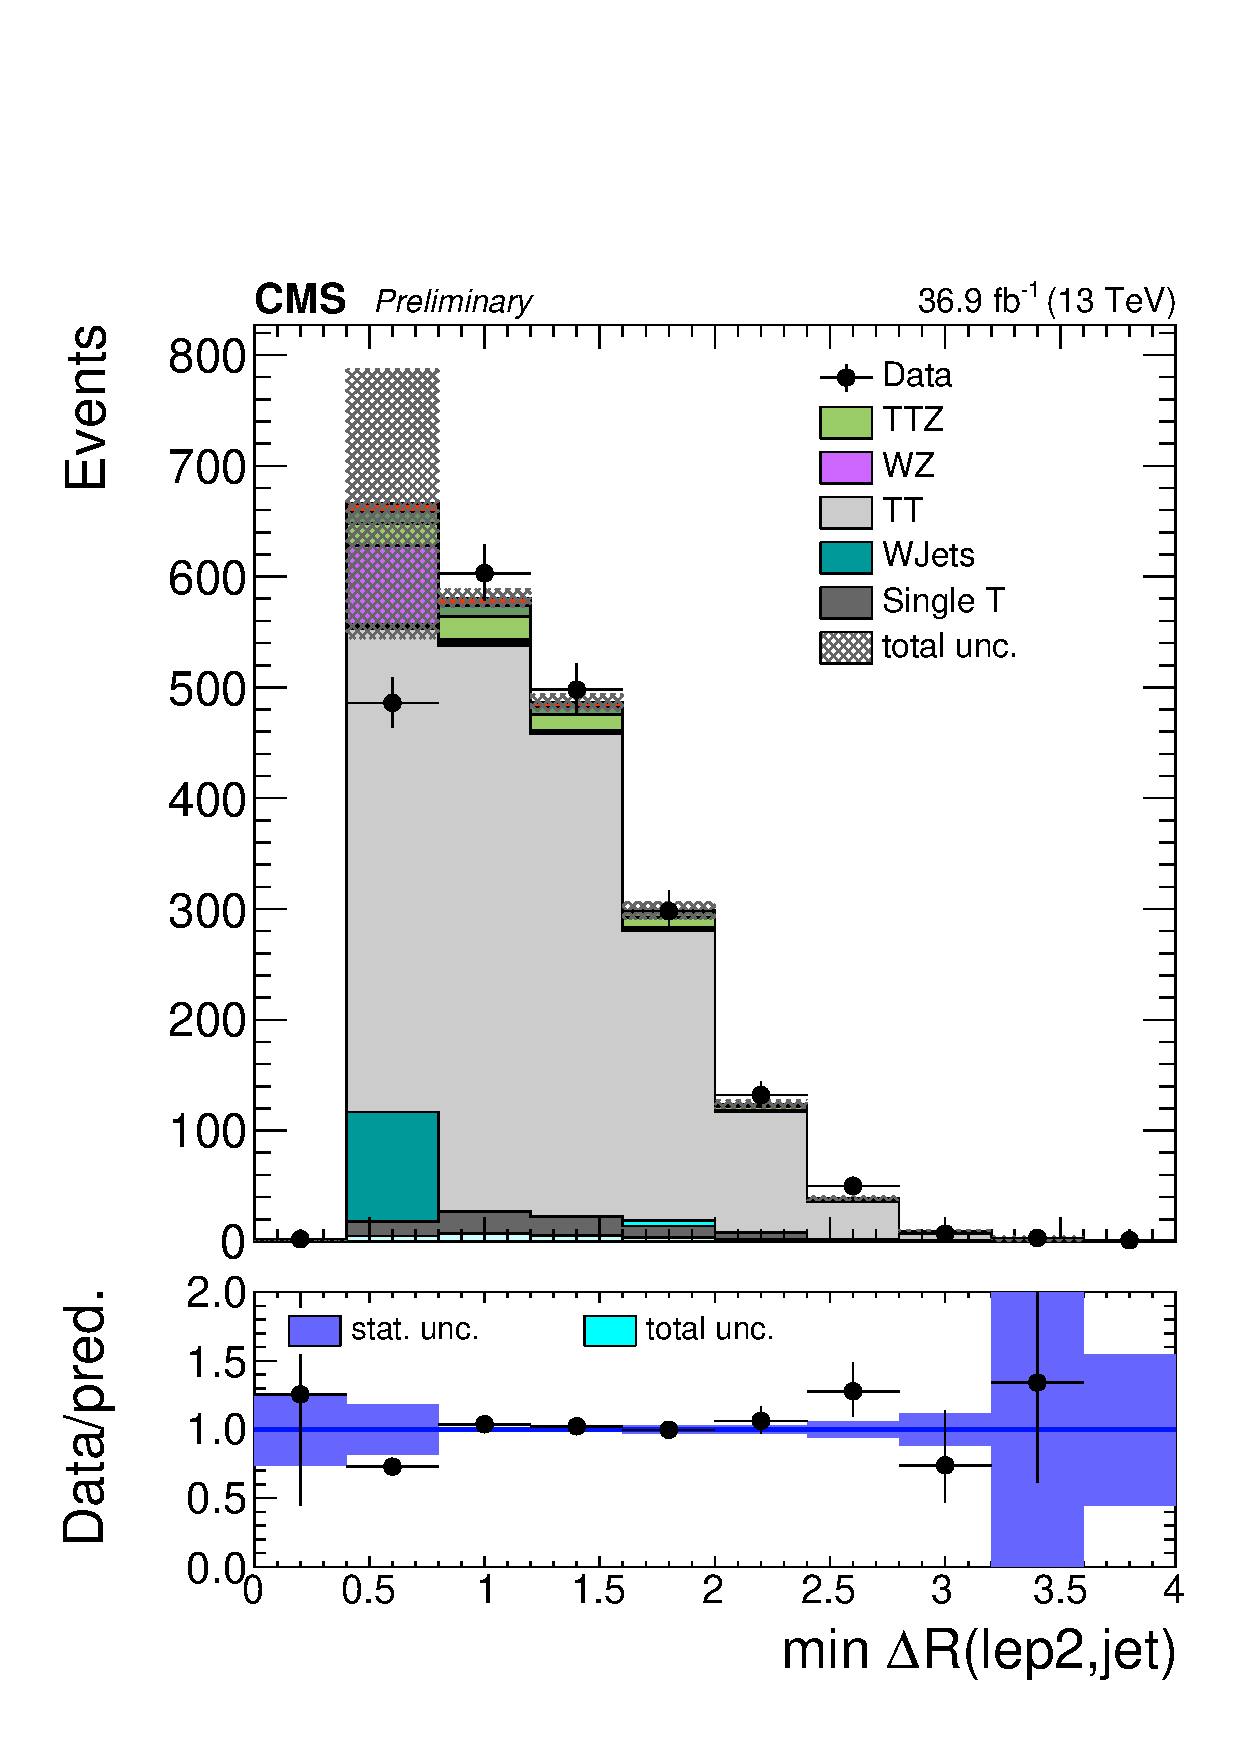
\includegraphics[width=0.30\linewidth]{plots_controlregions/2lss_appl_1fo_data/kinMVA_input_mindr_lep2_jet.pdf}
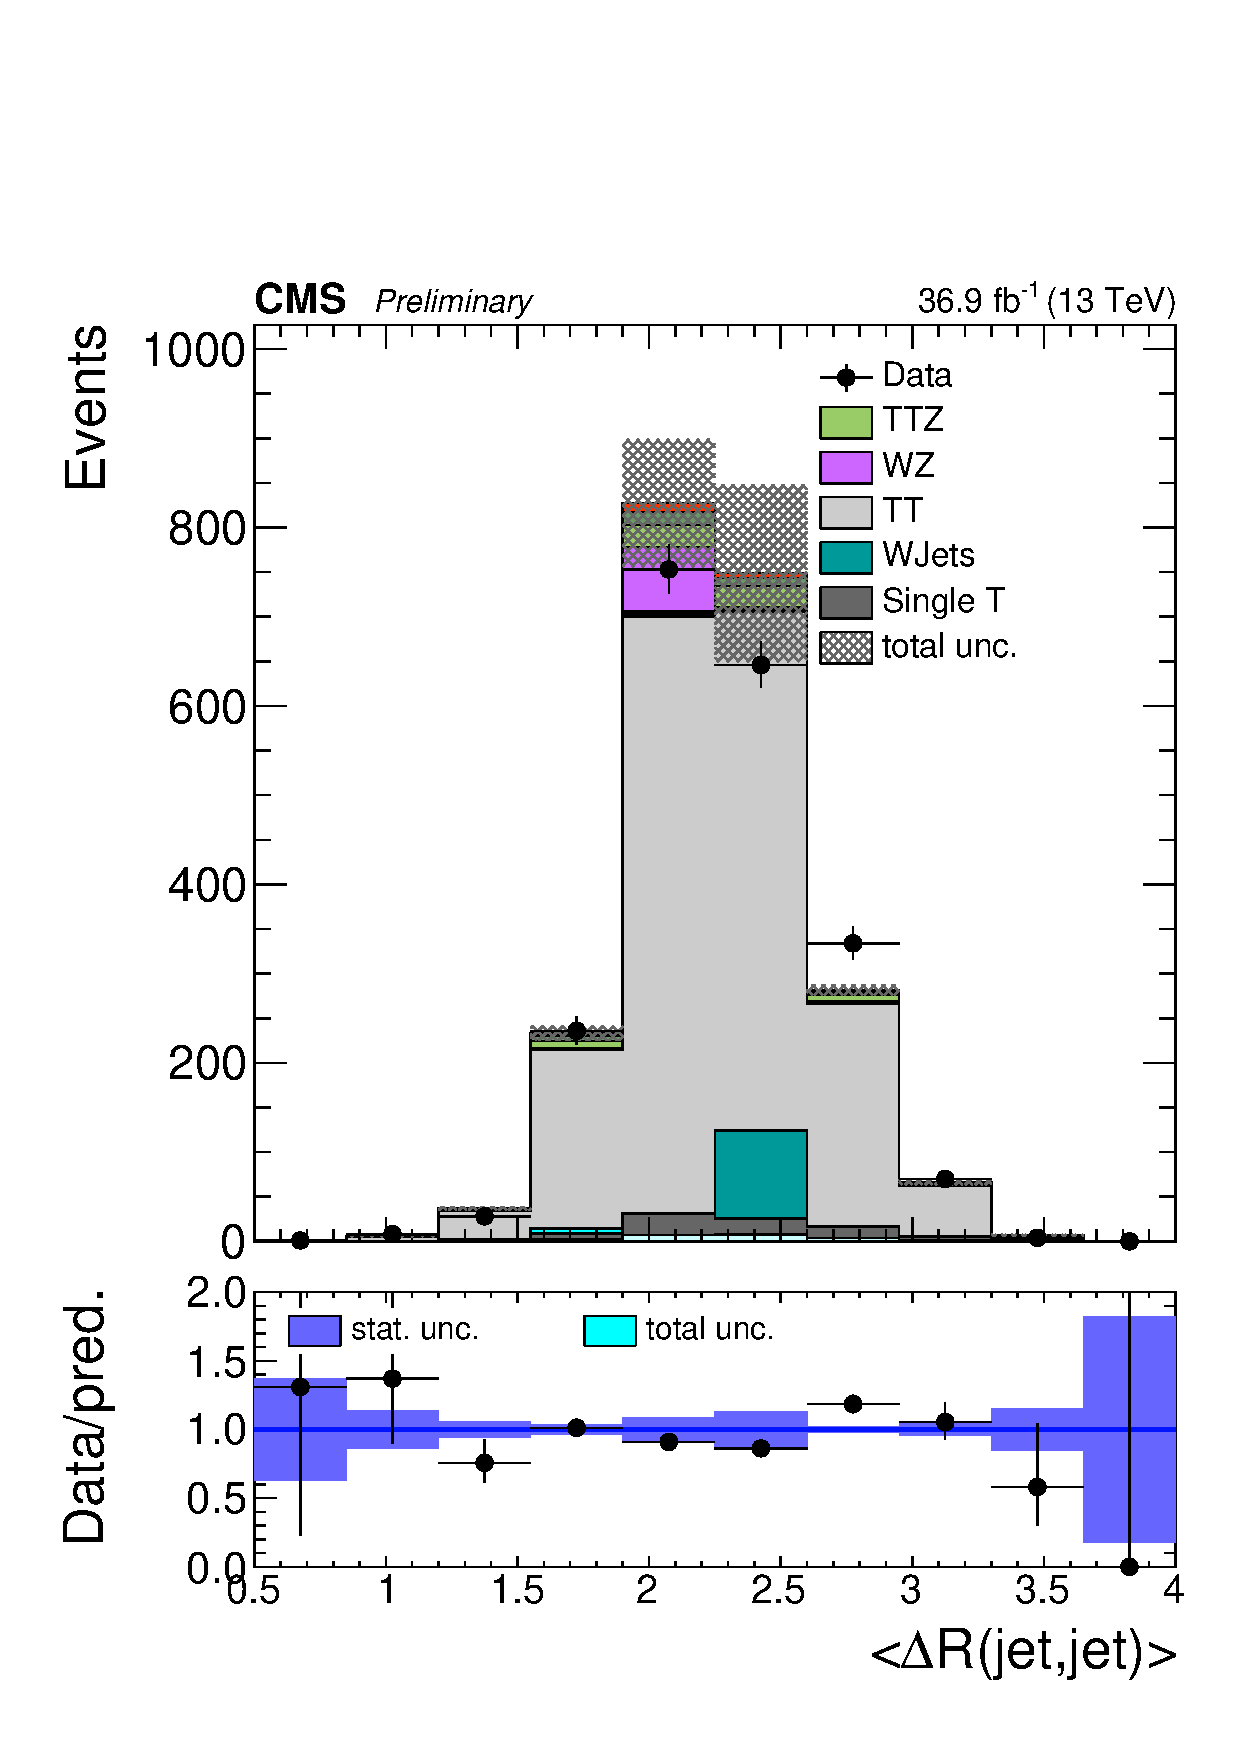
\includegraphics[width=0.30\linewidth]{plots_controlregions/2lss_appl_1fo_data/kinMVA_input_avg_dr_jet.pdf}
\caption{Distributions of several BDT input variables in the 2lss control region with exactly one fakeable lepton failing the tight selection requirements.
Uncertainties are statistical only.
}
\label{fig:cr_2lss_appl_1fo_3}
\end{figure}

%When further relaxing the selection to allow one or both leptons to fail the tight lepton requirements, the relative QCD contribution increases, as can be inferred by the plots shown in Fig.~\ref{fig:cr_2lss_appl}.

%\begin{figure}[!htb]
%\centering
%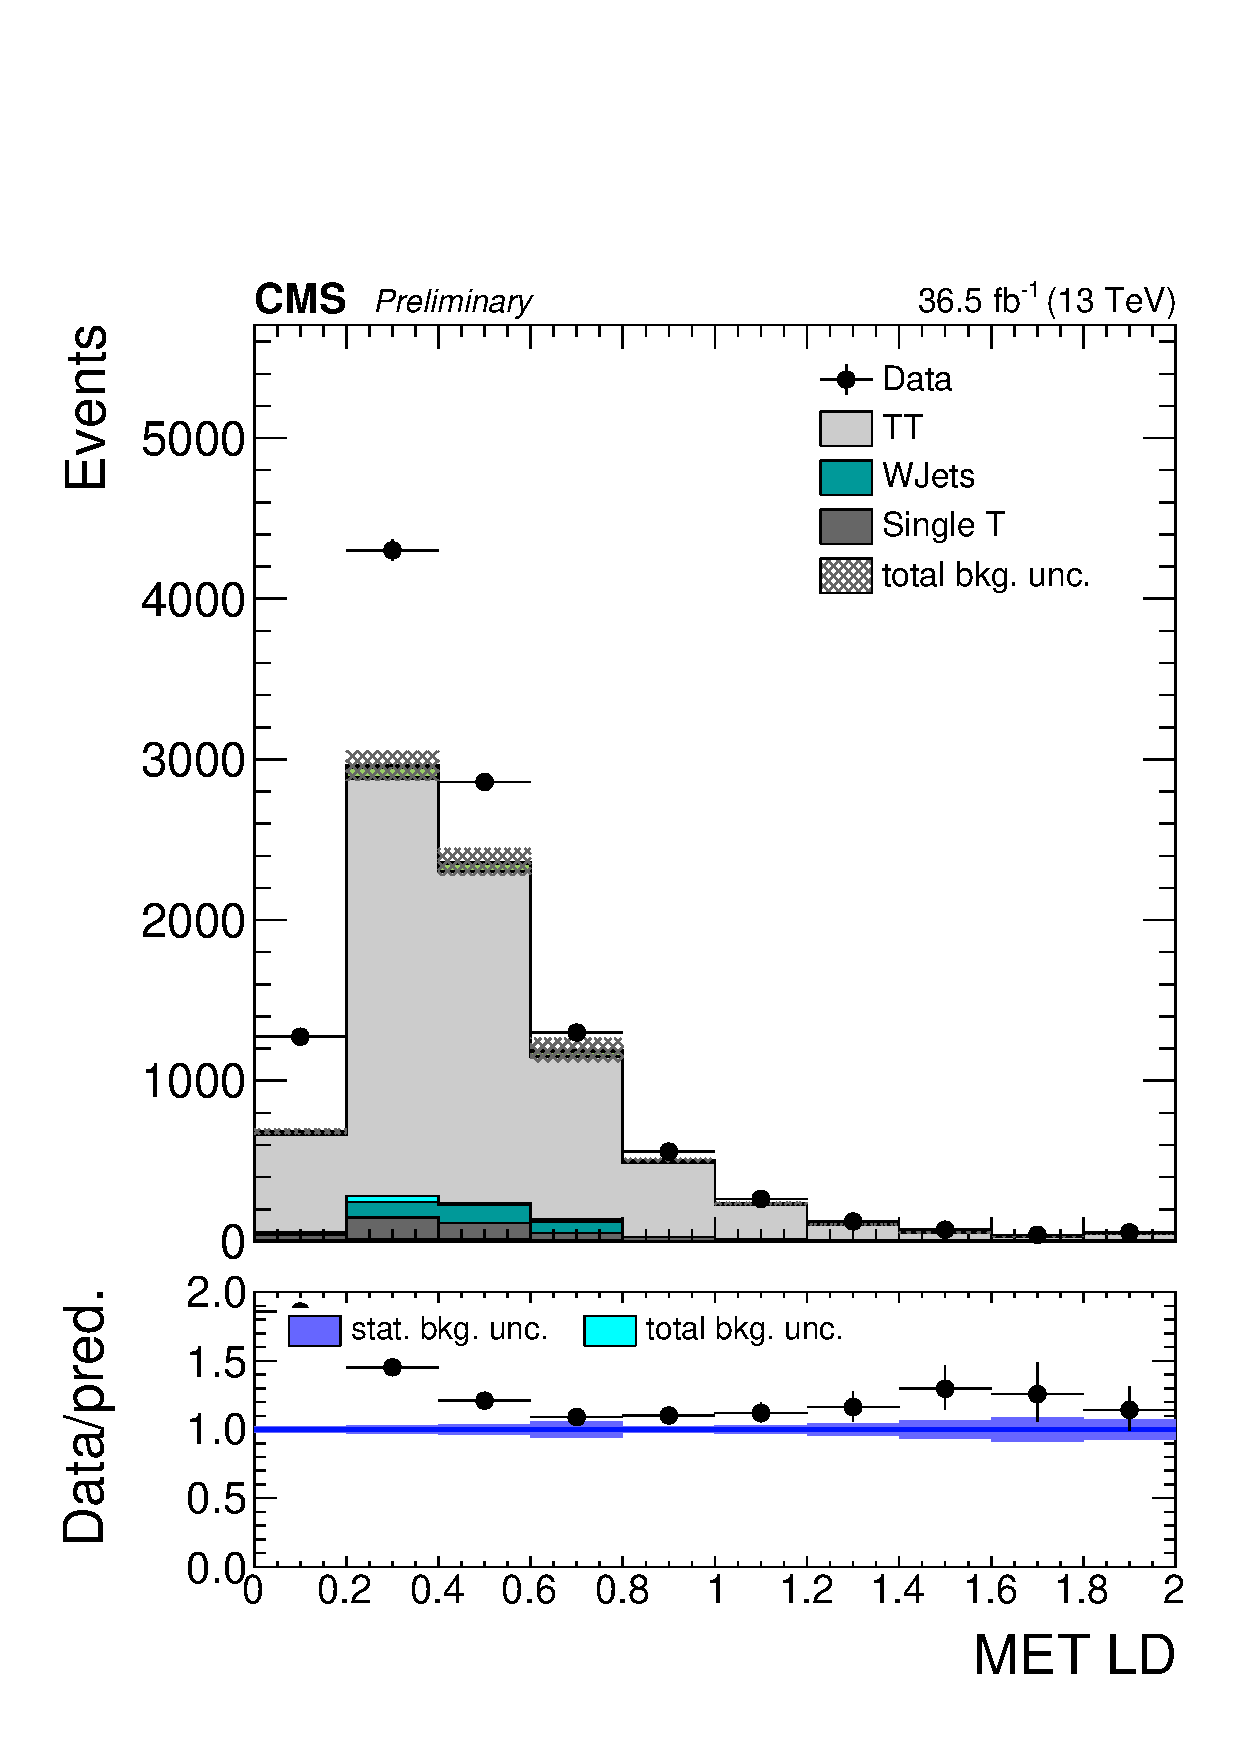
\includegraphics[width=0.30\linewidth]{plots_controlregions/2lss_appl_data/metLD.pdf}
%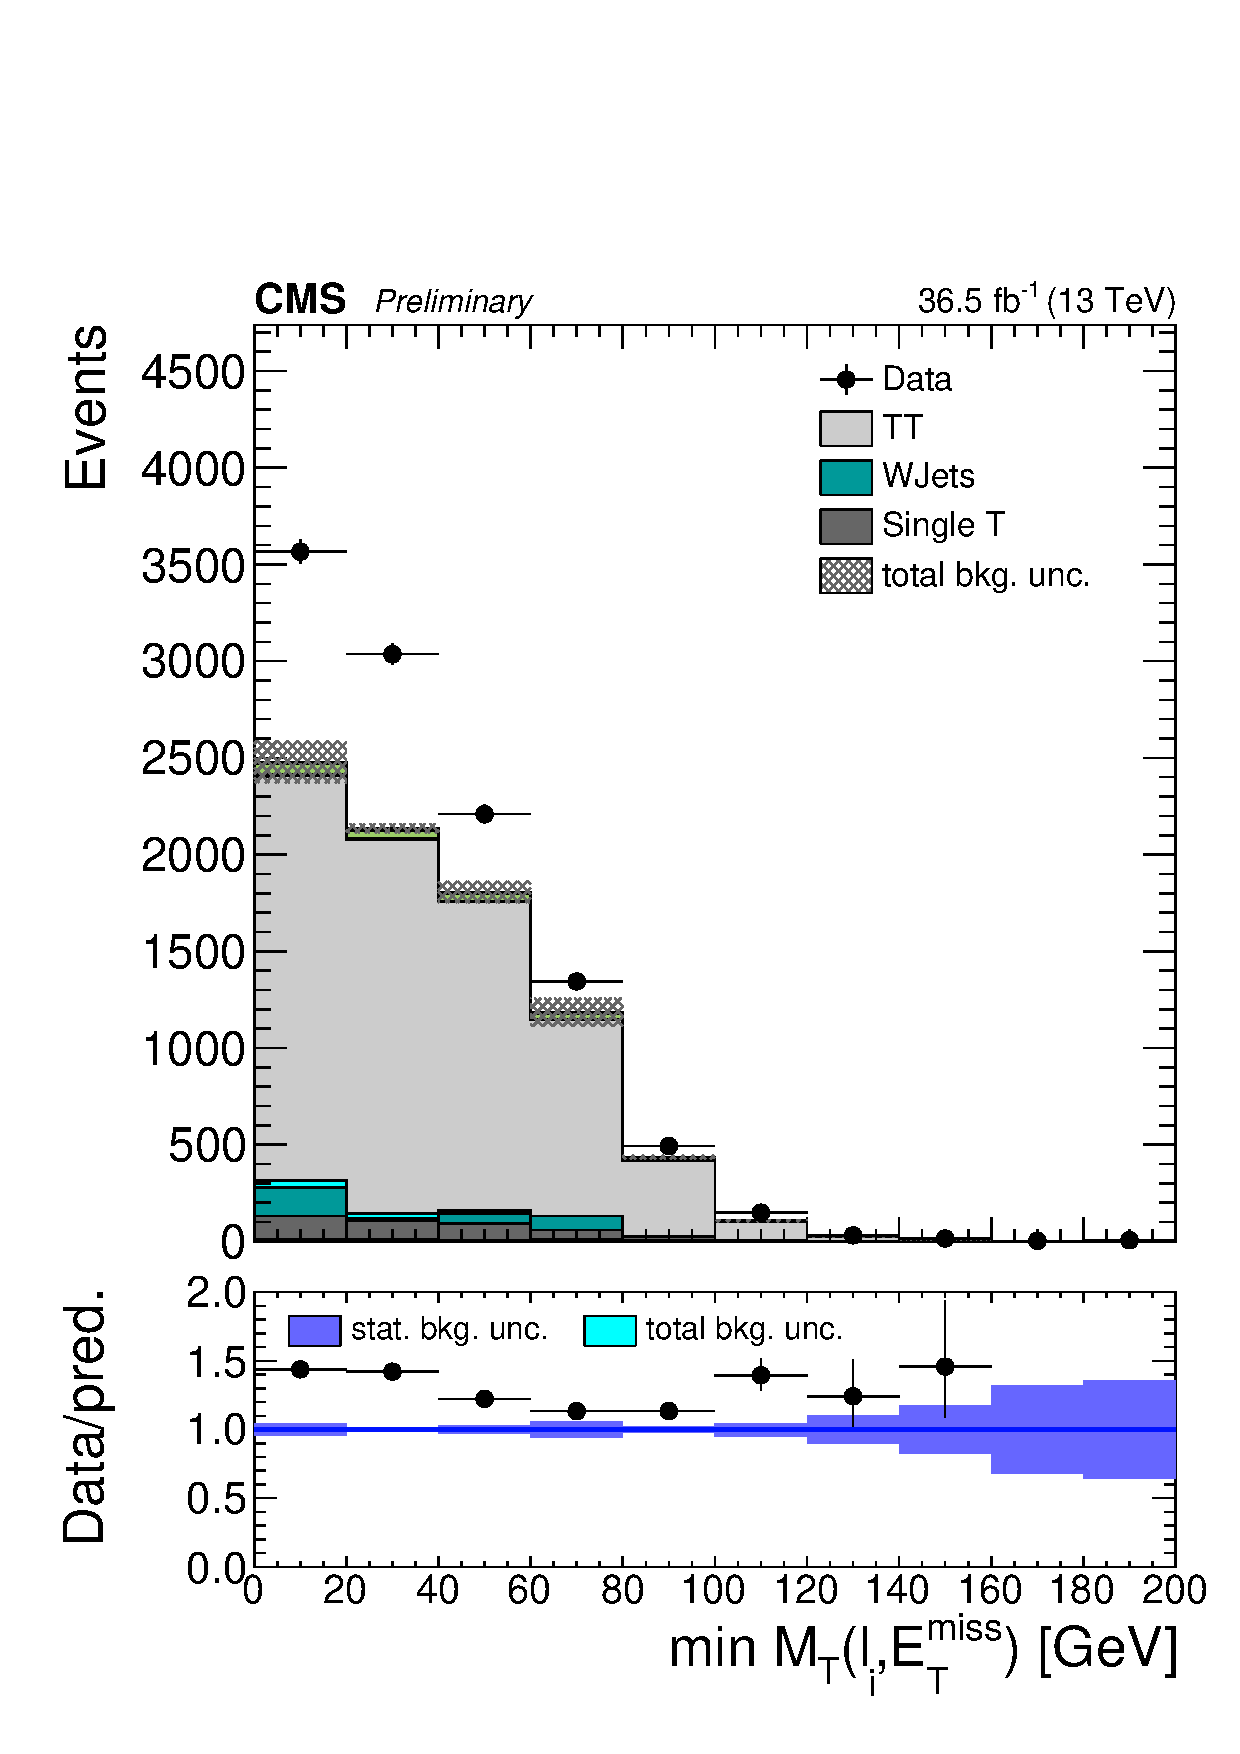
\includegraphics[width=0.30\linewidth]{plots_controlregions/2lss_appl_data/2lep_mtWmin.pdf}
%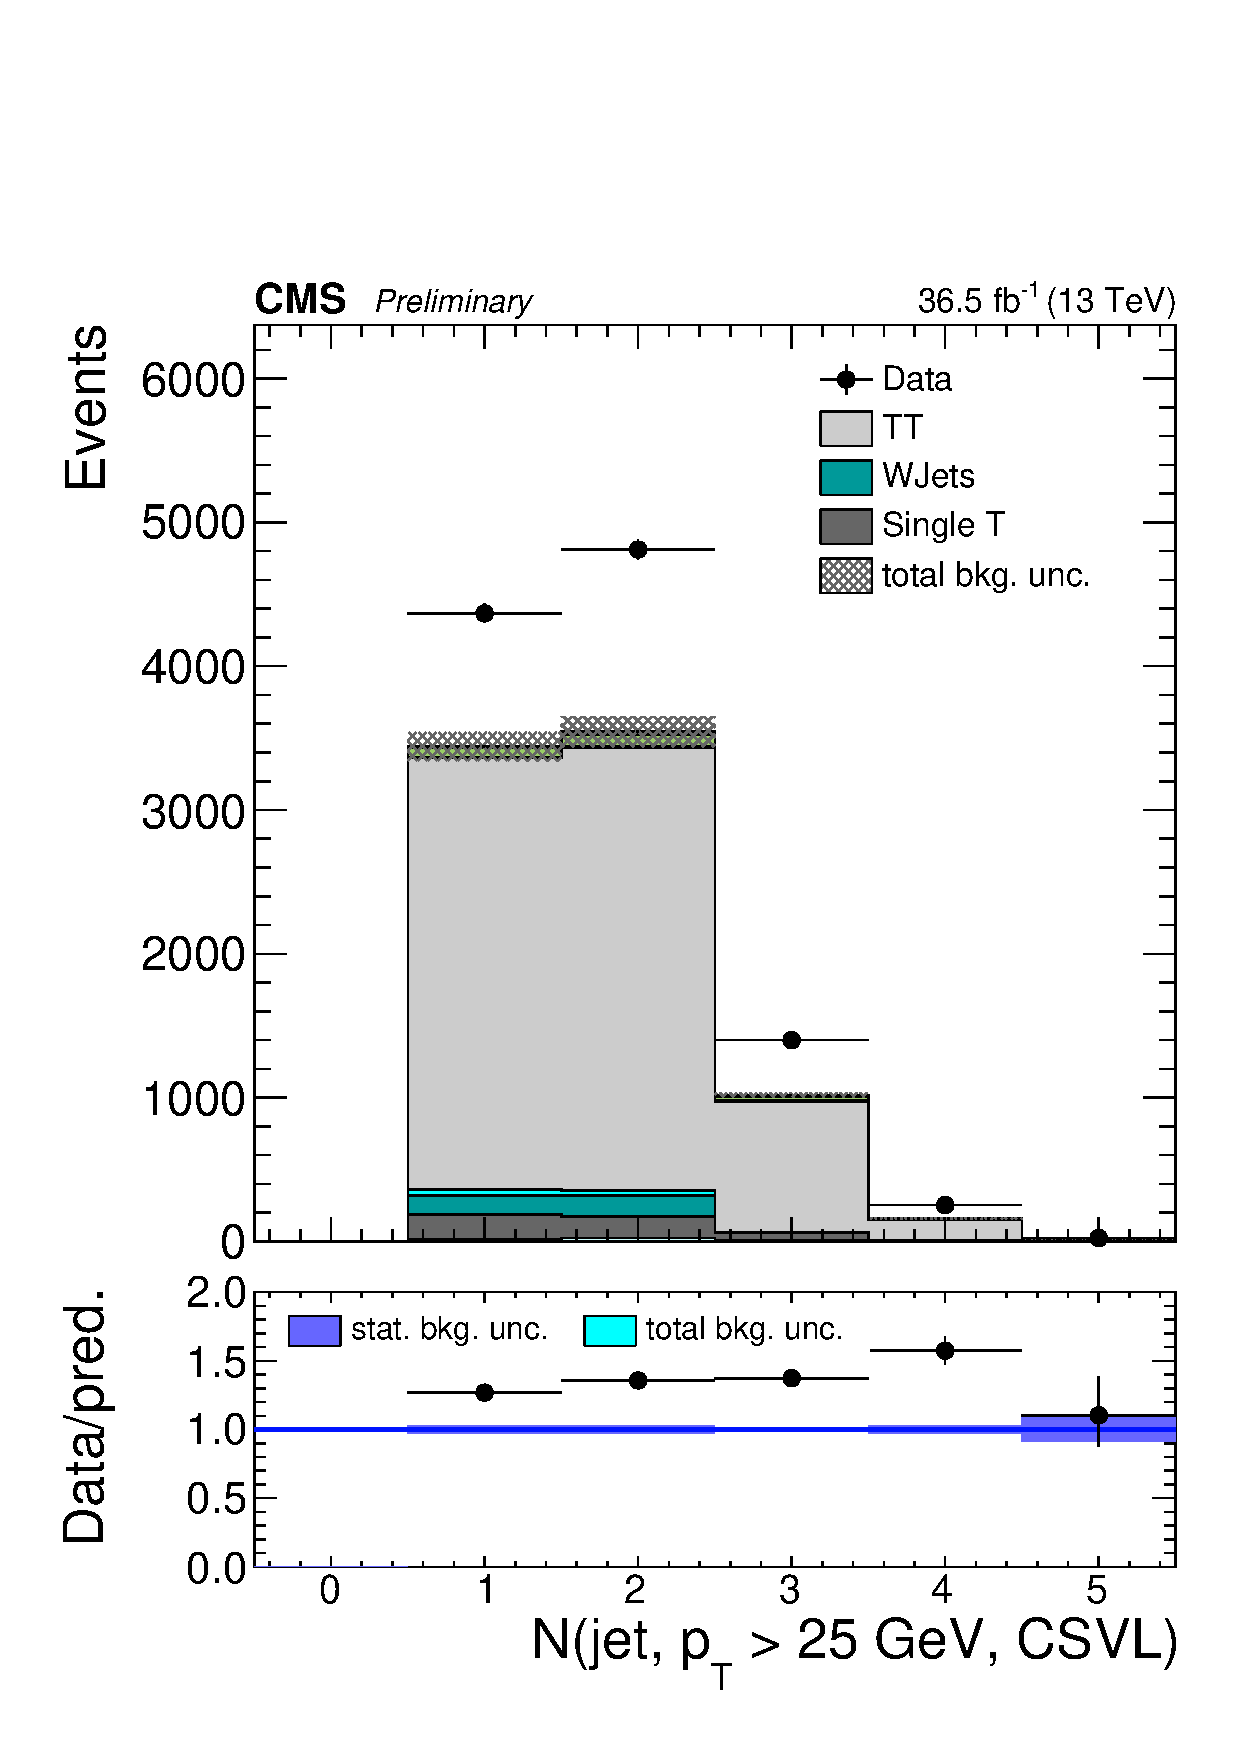
\includegraphics[width=0.30\linewidth]{plots_controlregions/2lss_appl_data/nBJetLoose25.pdf}
%\caption{Distributions and simulation distributions in the 2lss control region where at least one fakeable lepton fails the tight selection requirements.
%Uncertainties are statistical only. QCD multi-jet events that are not included among the simulated physics processes here.
%}
%\label{fig:cr_2lss_appl}
%\end{figure}



%%%%%%%%%%%%%%%%%%%%%%%%%%%%%%%%%%%%%%%%%%%%%%%%%%%%%%%%%%%%%%%
\clearpage
%%%%%%%%%%%%%%%%%%%%%%%%%%%%%%%%%%%%%%%%%%%%%%%%%%%%%%%%%%%%%%%

\subsection{Jet multiplicity sideband region}

This 2lss control region is enriched in fakes from $\ttbar$. It is obtained by requiring exactly three reconstructed jets in the final state,
in the place of the requirement of at least four that is applied in the standard 2lss selection.

Fakes from W+jets are estimated by the fake rate method described in Section~\ref{sec:fakerate}, applied on MC events, while all other processes are predicted by the simulation.
Distributions of event observables are shown in Fig.~\ref{fig:cr_2lss_3j_1}-\ref{fig:cr_2lss_3j_3}.
In all cases we observe a satisfactory data/MC agreement, within the statistics currently available.

\begin{figure}[!htb]
\centering
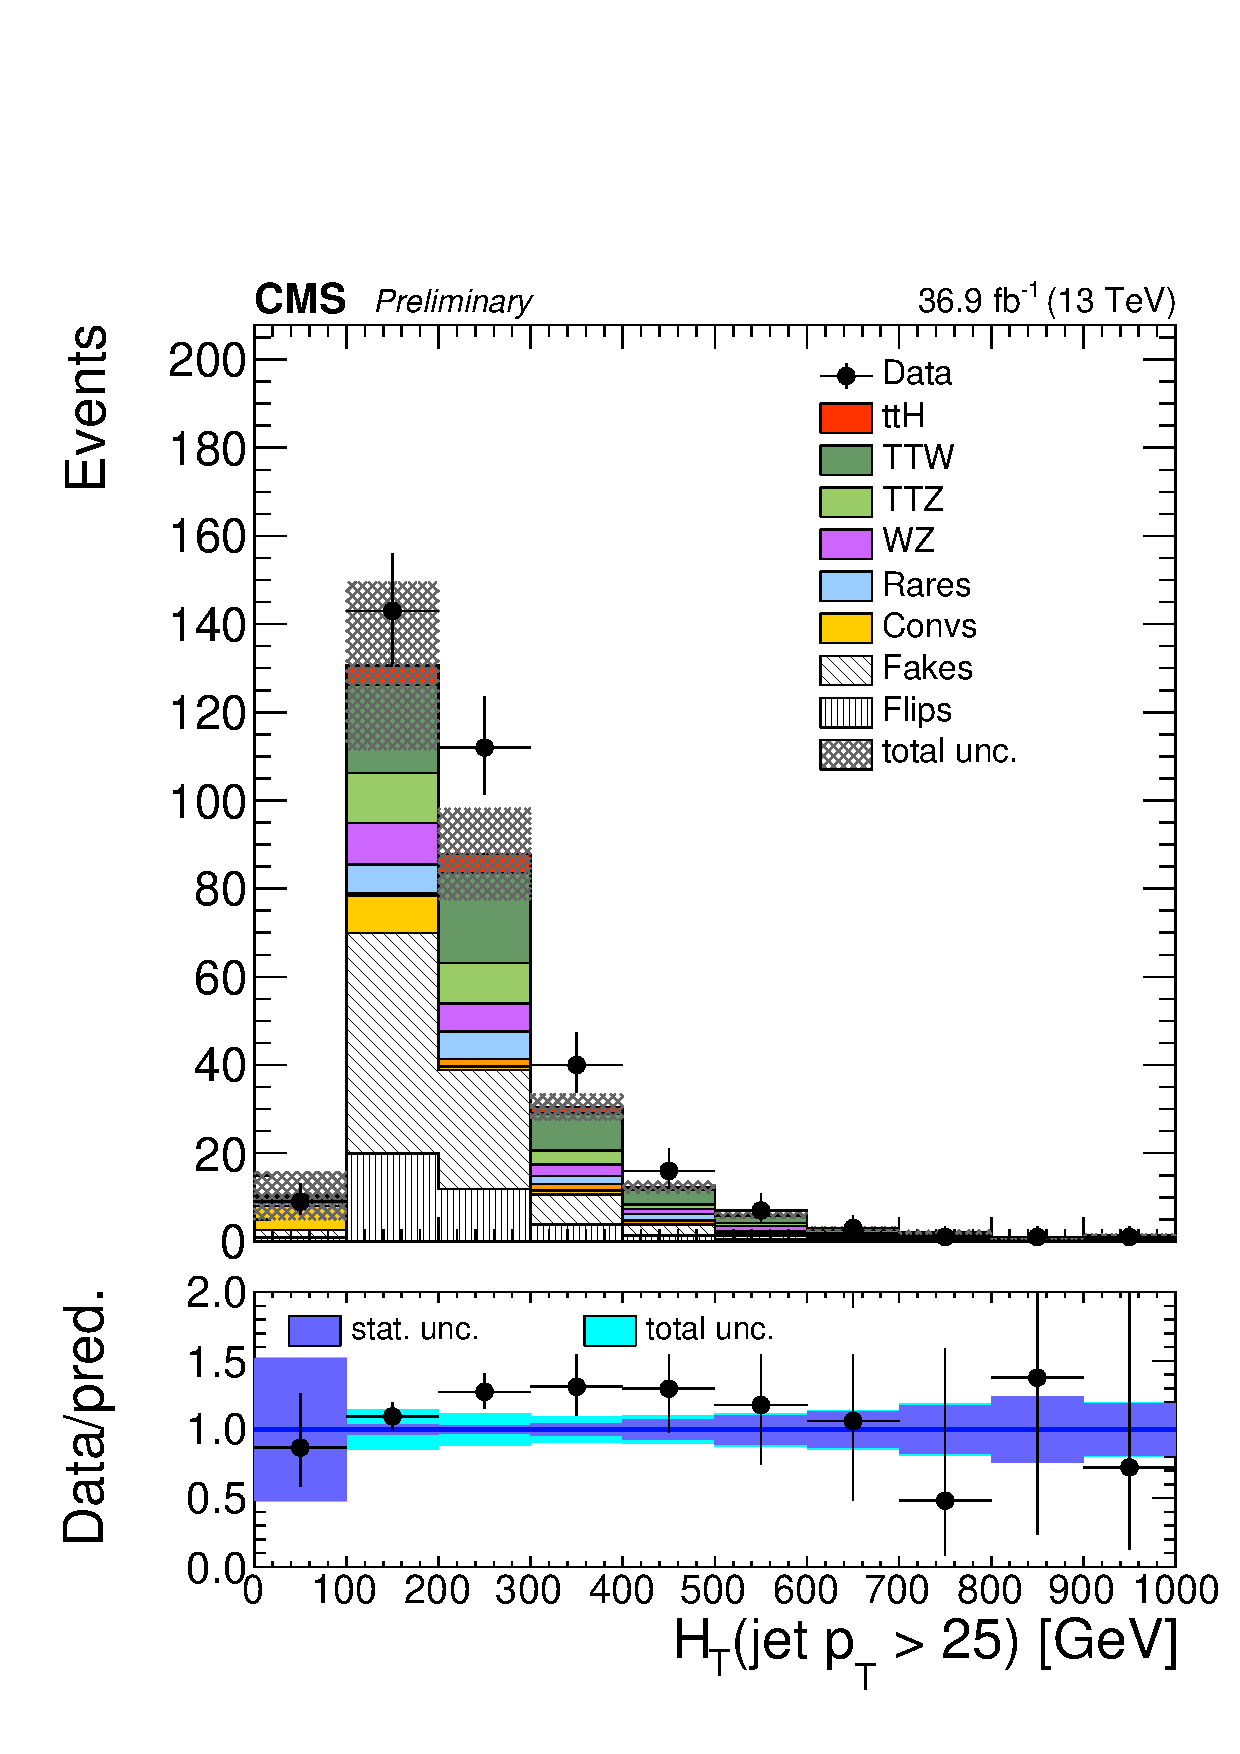
\includegraphics[width=0.30\linewidth]{plots_controlregions/cr_3j_data_frdata/htJet25j.pdf}
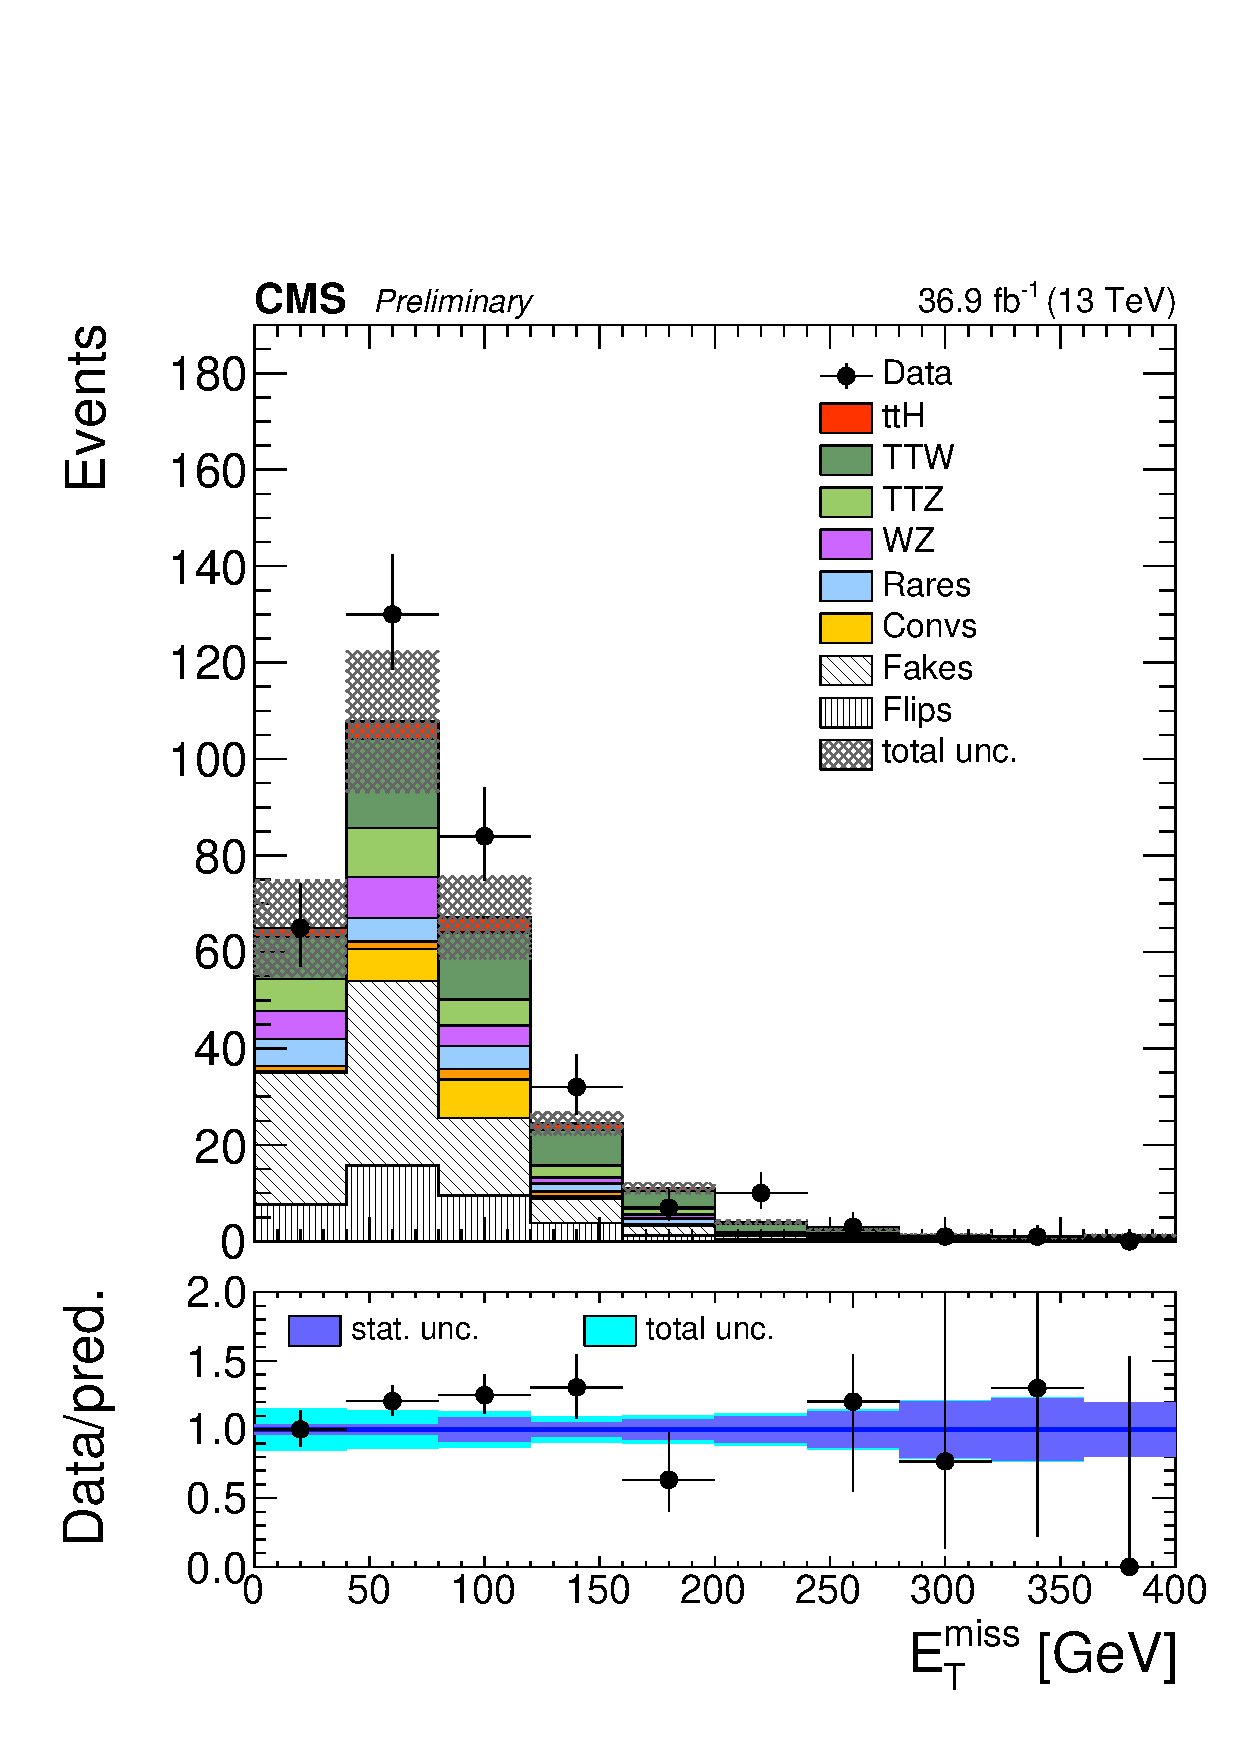
\includegraphics[width=0.30\linewidth]{plots_controlregions/cr_3j_data_frdata/met.pdf}
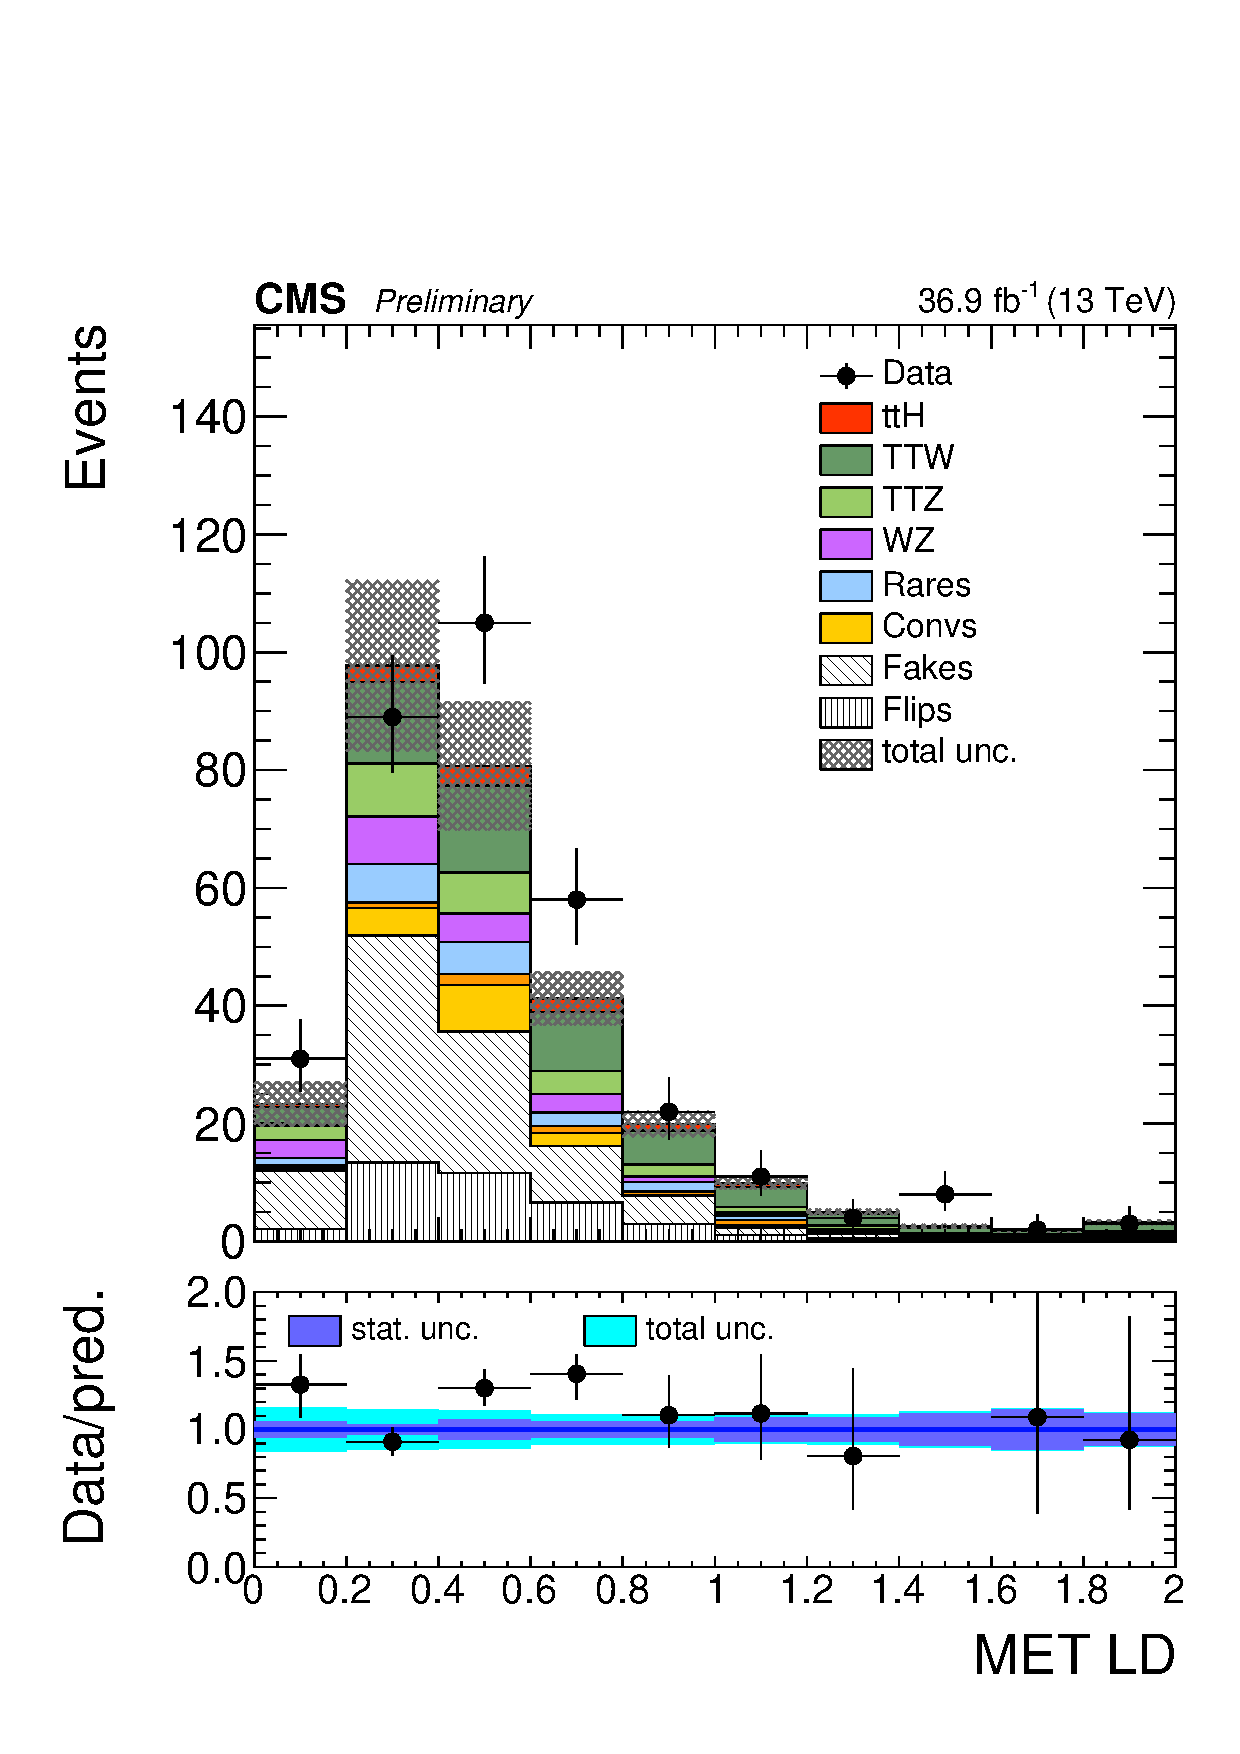
\includegraphics[width=0.30\linewidth]{plots_controlregions/cr_3j_data_frdata/metLD.pdf}\\
\caption{Distributions in the 2lss control region with exactly three jets in the final state.
From left to right: the $H_T$, the $E_{T}^{miss}$, the $E_{T}^{miss}LD$.
Uncertainties are statistical only.
}
\label{fig:cr_2lss_3j_1}
\end{figure}

\begin{figure}[!htb]
\centering
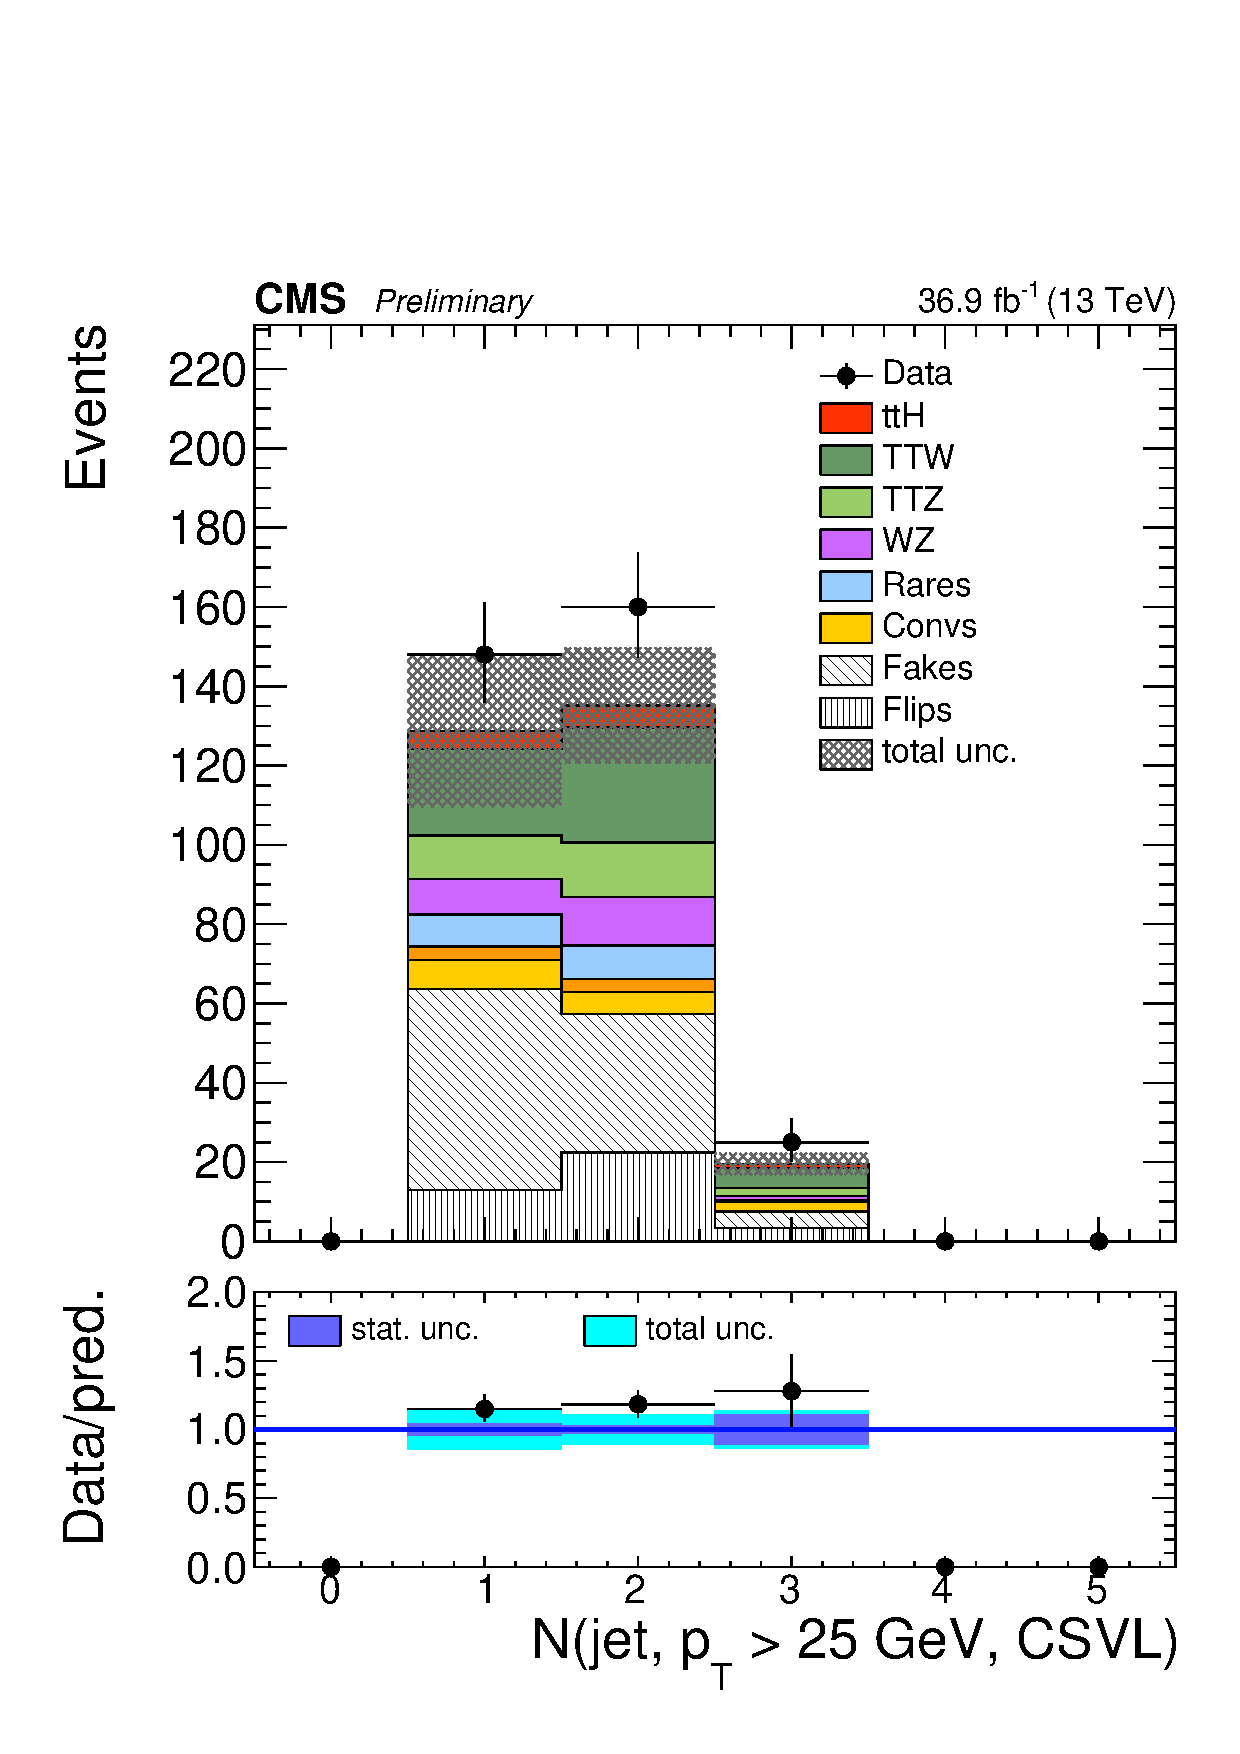
\includegraphics[width=0.35\linewidth]{plots_controlregions/cr_3j_data_frdata/nBJetLoose25.pdf}
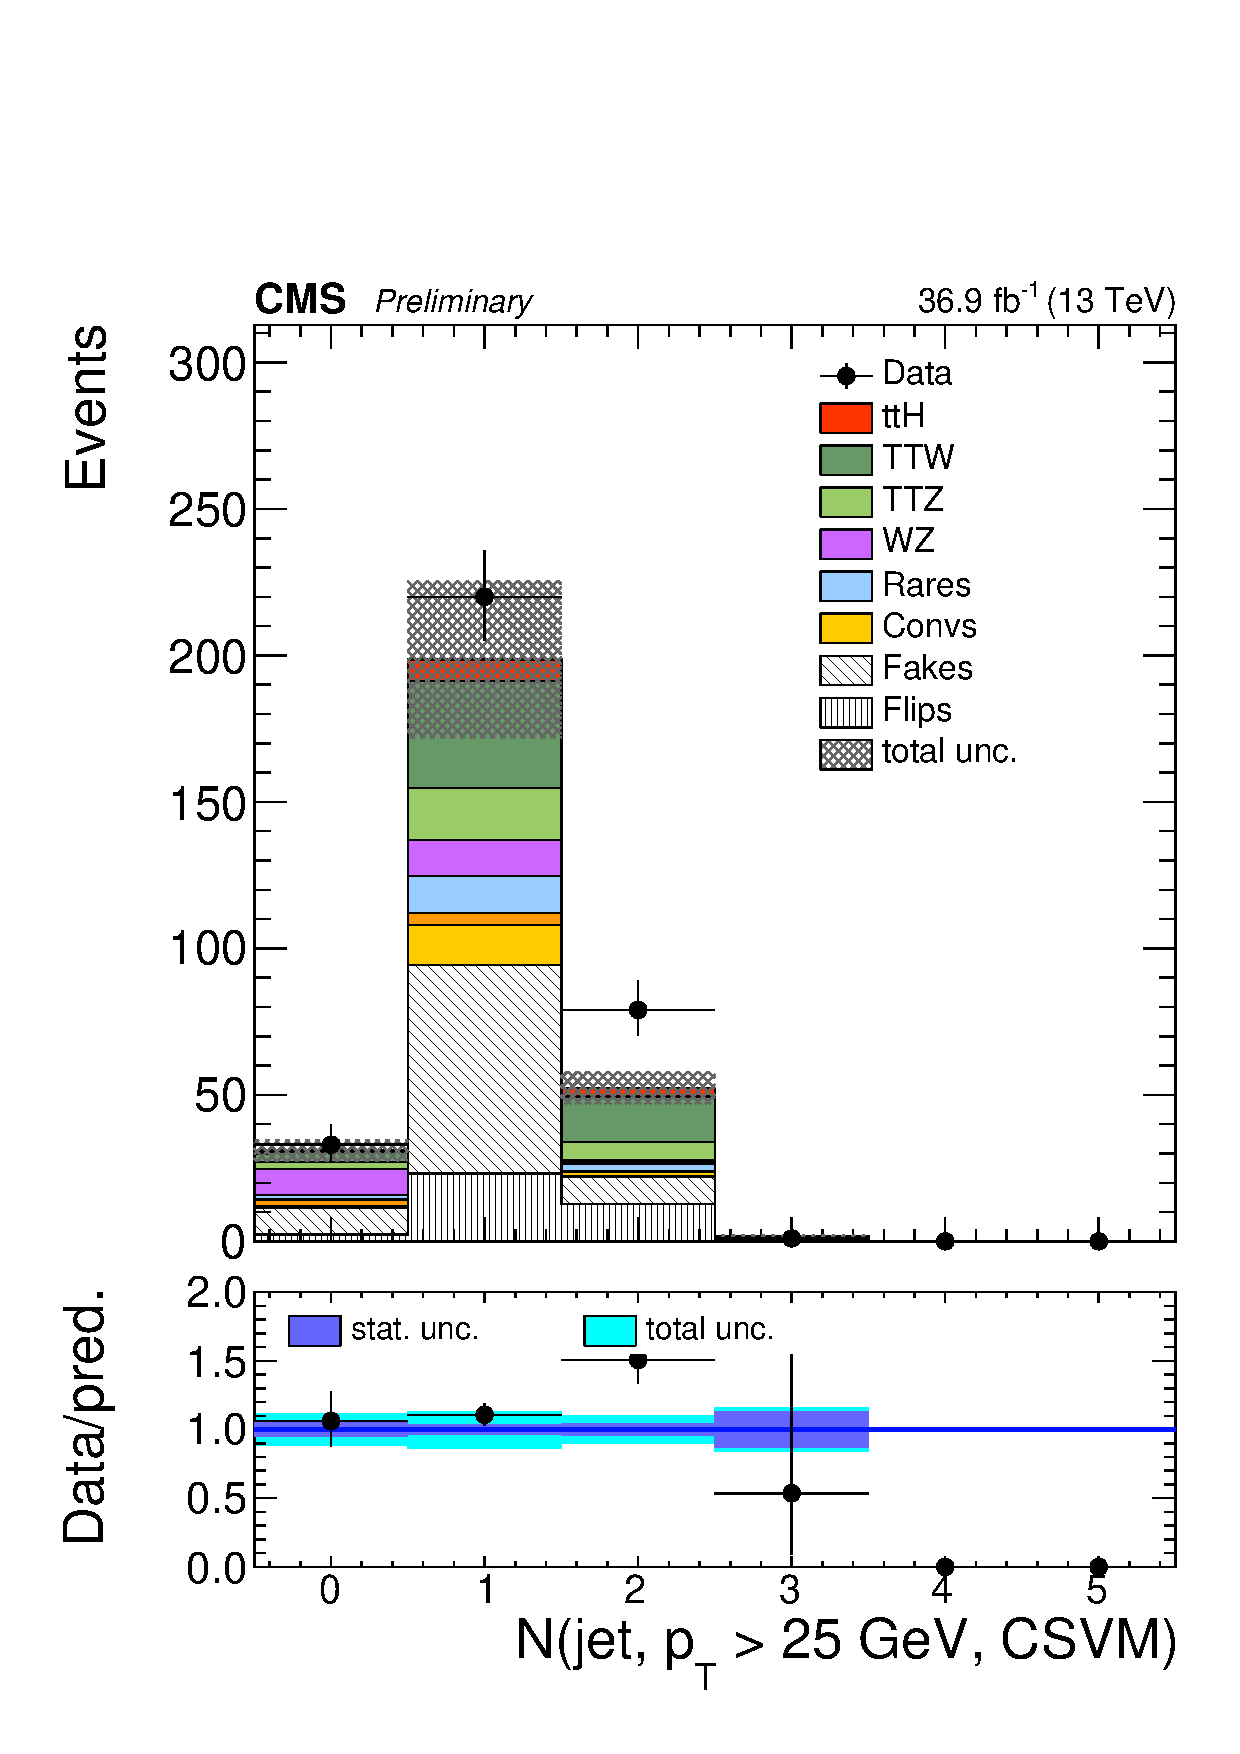
\includegraphics[width=0.35\linewidth]{plots_controlregions/cr_3j_data_frdata/nBJetMedium25.pdf}\\
\caption{Distributions for the number of jets passing the loose and medium working points of the CSV b-tagger, in the 2lss control region with exactly three jets in the final state.
Uncertainties are statistical only.
}
\label{fig:cr_2lss_3j_2}
\end{figure}

\begin{figure}[!htb]
\centering
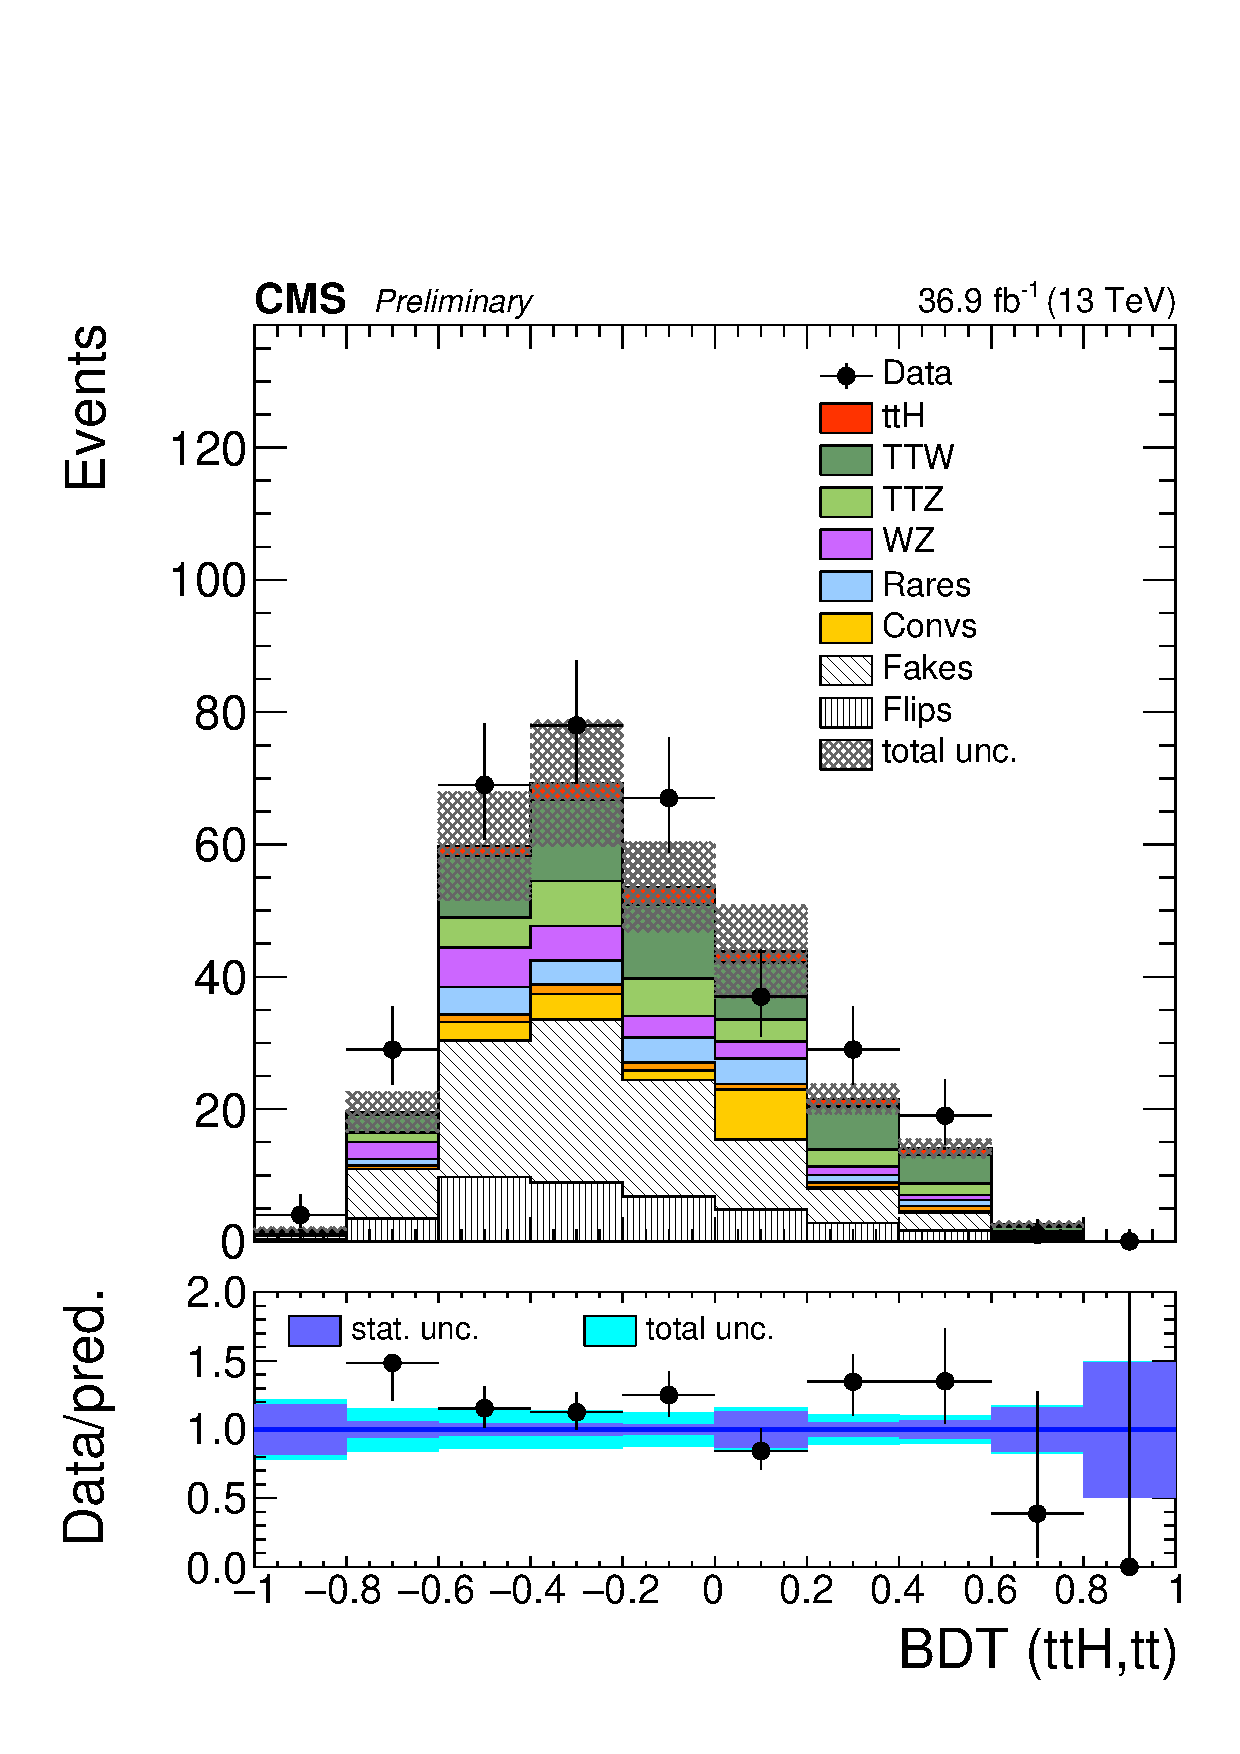
\includegraphics[width=0.35\linewidth]{plots_controlregions/cr_3j_data_frdata/kinMVA_2lss_ttbar.pdf}
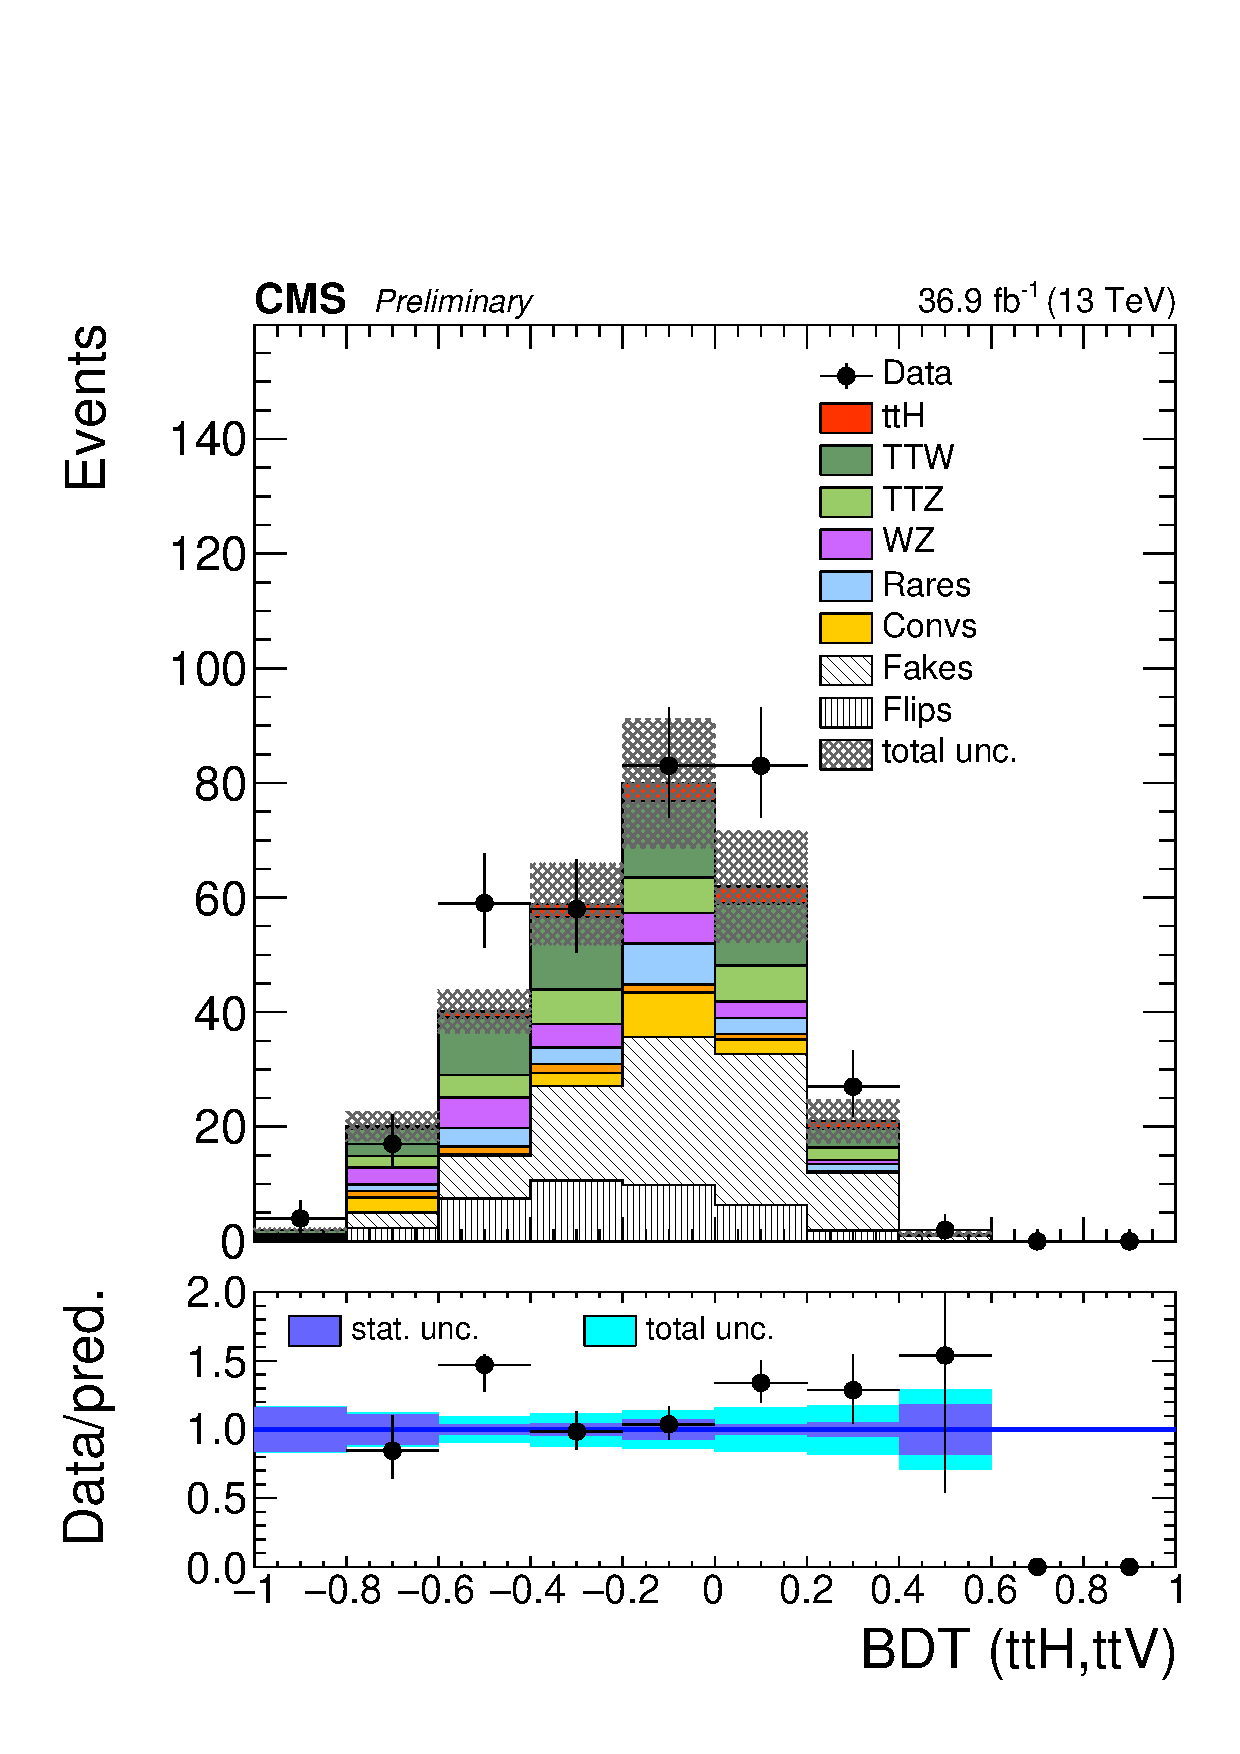
\includegraphics[width=0.35\linewidth]{plots_controlregions/cr_3j_data_frdata/kinMVA_2lss_ttV.pdf}
\caption{Distributions of the discriminators against $\ttbar$ and $ttV$ in the 2lss control region with exactly three jets in the final state.
Uncertainties are statistical only.
}
\label{fig:cr_2lss_3j_3}
\end{figure}

%%%%%%%%%%%%%%%%%%%%%%%%%%%%%%%%%%%%%%%%%%%%%%%%%%%%%%%%%%%%%%%%
%\clearpage
%%%%%%%%%%%%%%%%%%%%%%%%%%%%%%%%%%%%%%%%%%%%%%%%%%%%%%%%%%%%%%%%
%
%\subsection{\texorpdfstring{$\ttbar\to\Pe^\pm\Pgm^\mp\,\cPqb\cPaqb\,\Pgn\Pagn$}{tt->em 2b 2v}}
%
%This control region is enriched in $\ttbar$ events, and aims at validating the jet-related observables used in the analysis.
%The selection we apply is the same as in the 2lss category of the analysis, with the following modifications:\\
%\begin{itemize}
%\item the two selected leptons are required to be of opposite sign and flavor (one electron and one muon);
%\item the requirement on the number of jets is relaxed to $\geq 2$;
%\item the requirements on the number of b-jets is relaxed to at least one jet passing the medium working point of the CSV tagger;
%\end{itemize}
%
%Distributions of some event observables are shown in Fig.~\ref{fig:cr_tt2l}.
%
%\begin{figure}[!htb]
%\centering
%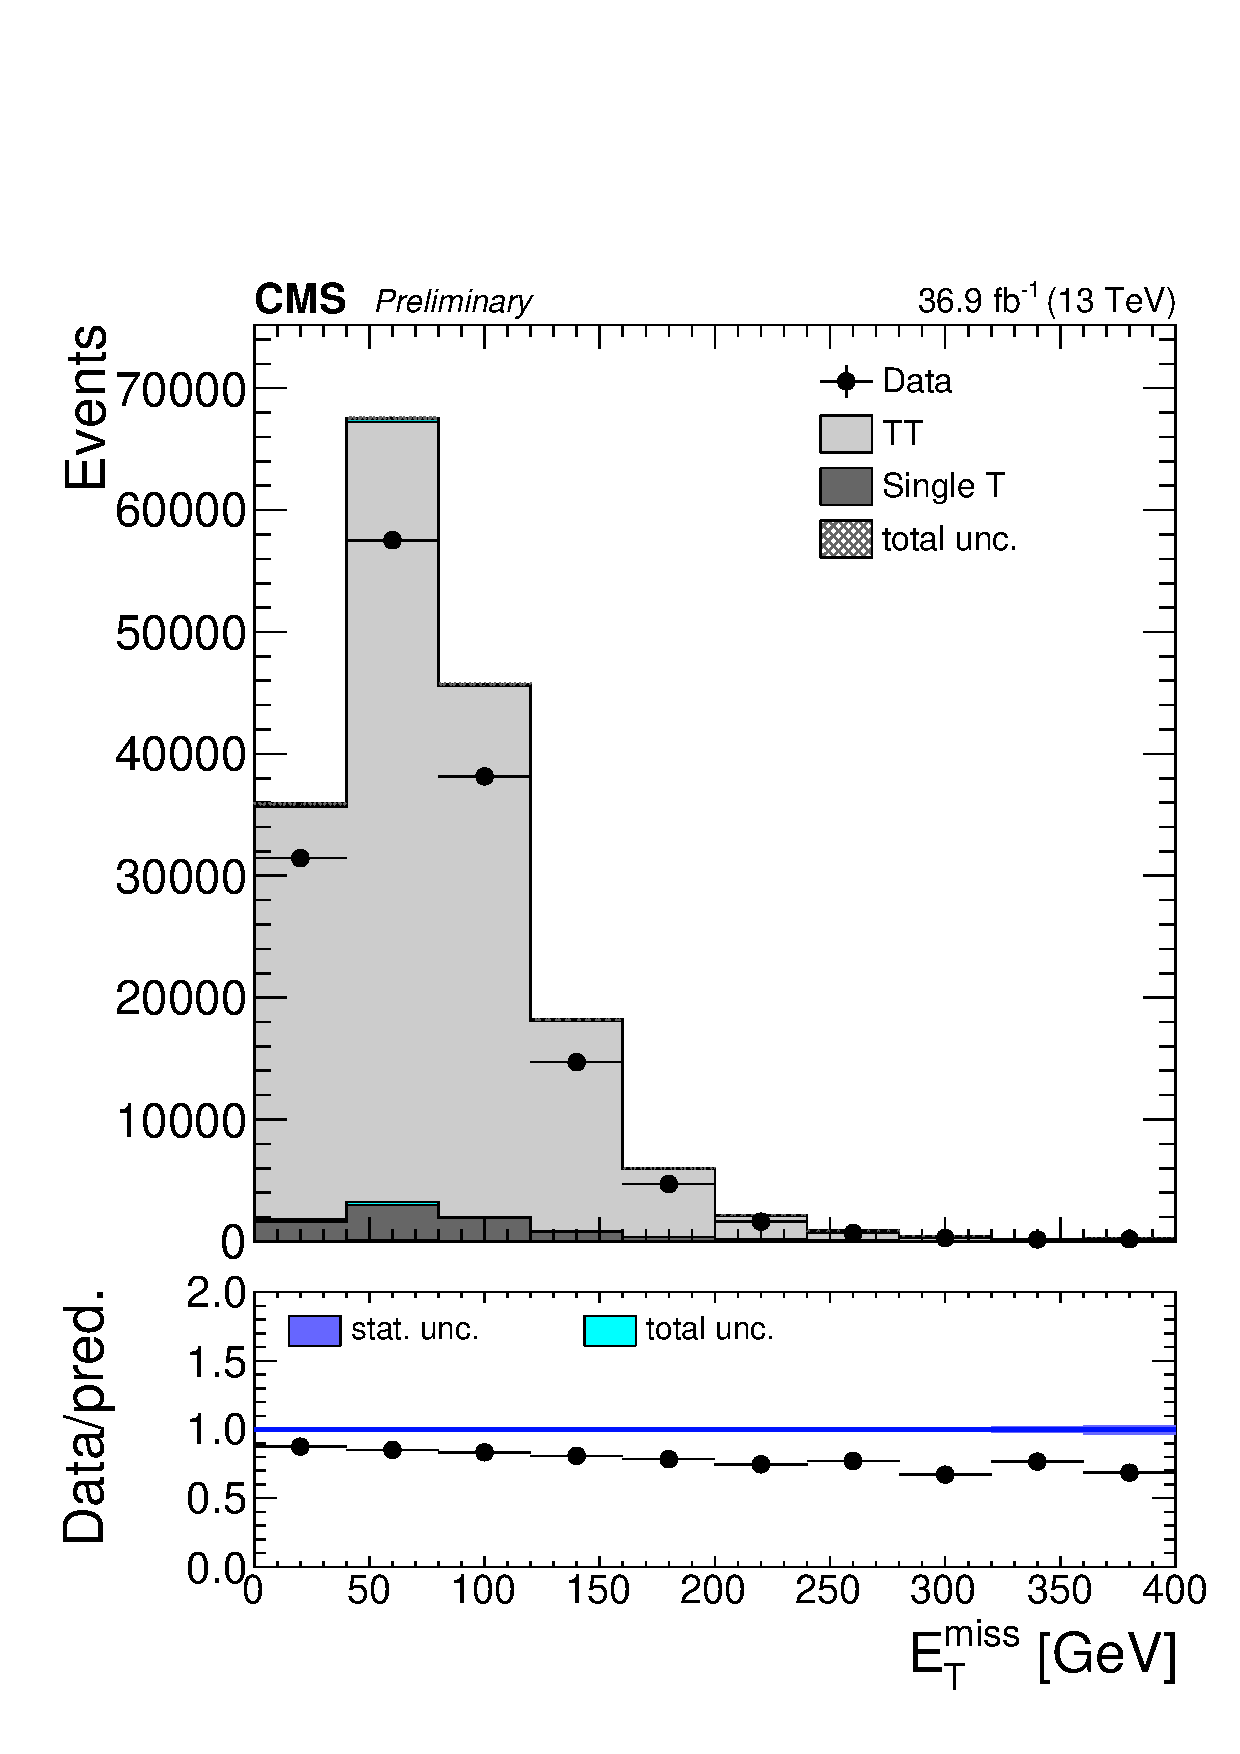
\includegraphics[width=0.35\linewidth]{plots_controlregions/cr_ttbar_data/met.pdf}
%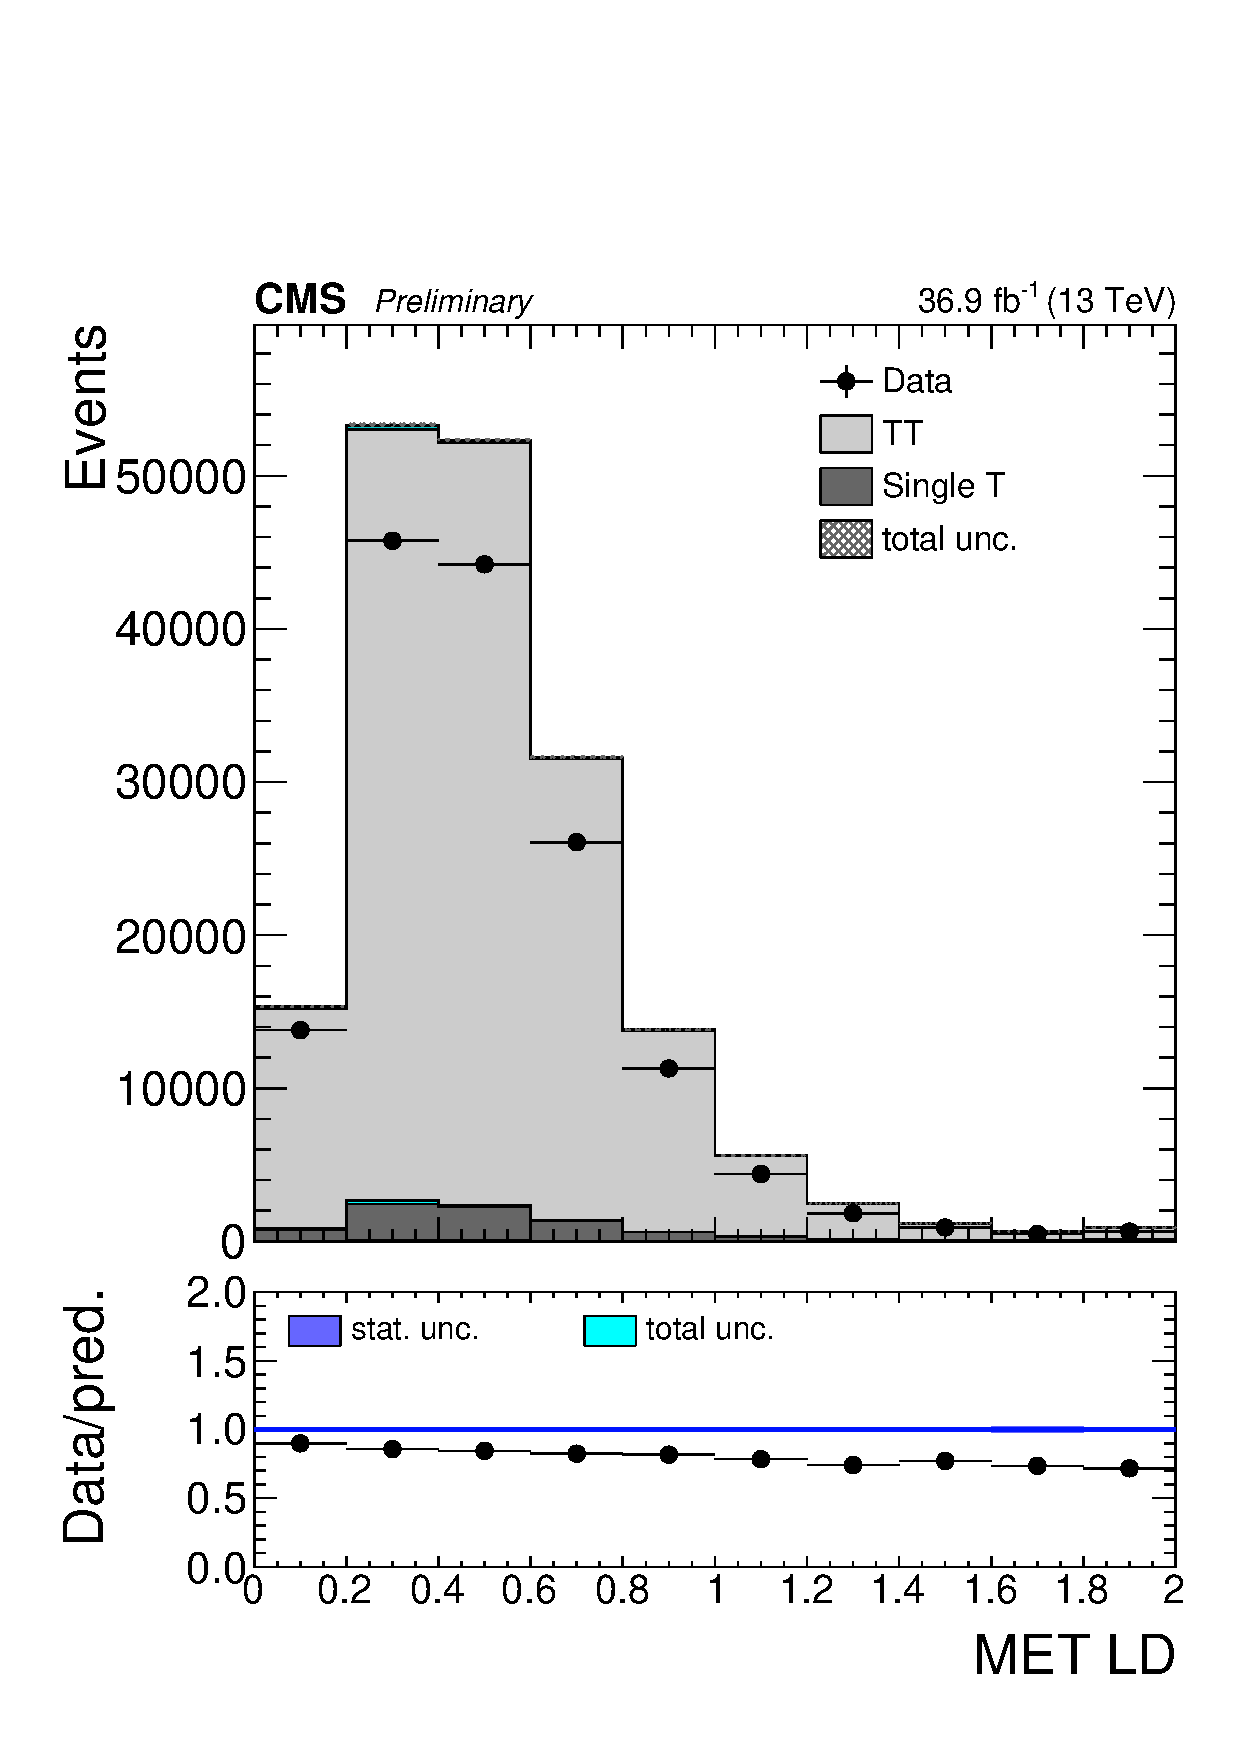
\includegraphics[width=0.35\linewidth]{plots_controlregions/cr_ttbar_data/metLD.pdf}\\
%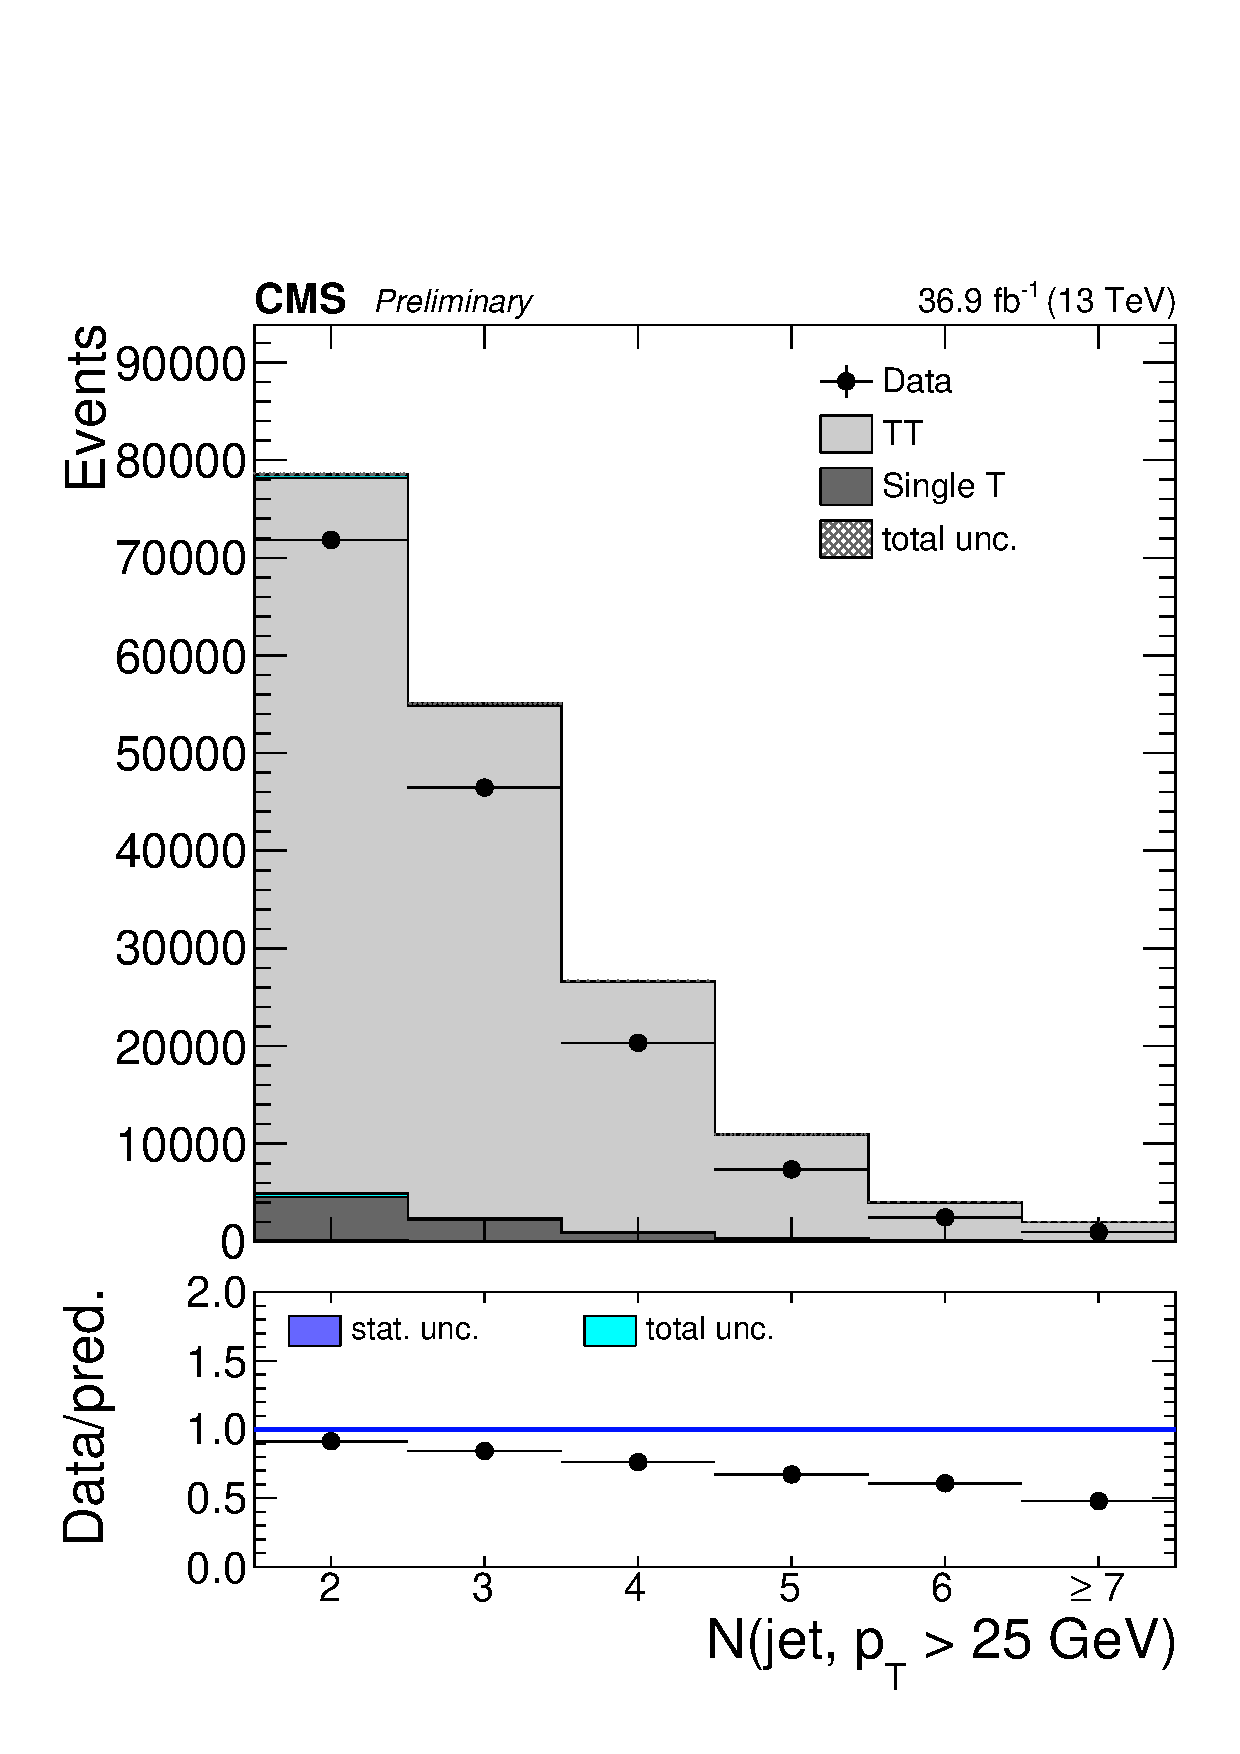
\includegraphics[width=0.35\linewidth]{plots_controlregions/cr_ttbar_data/nJet25.pdf}
%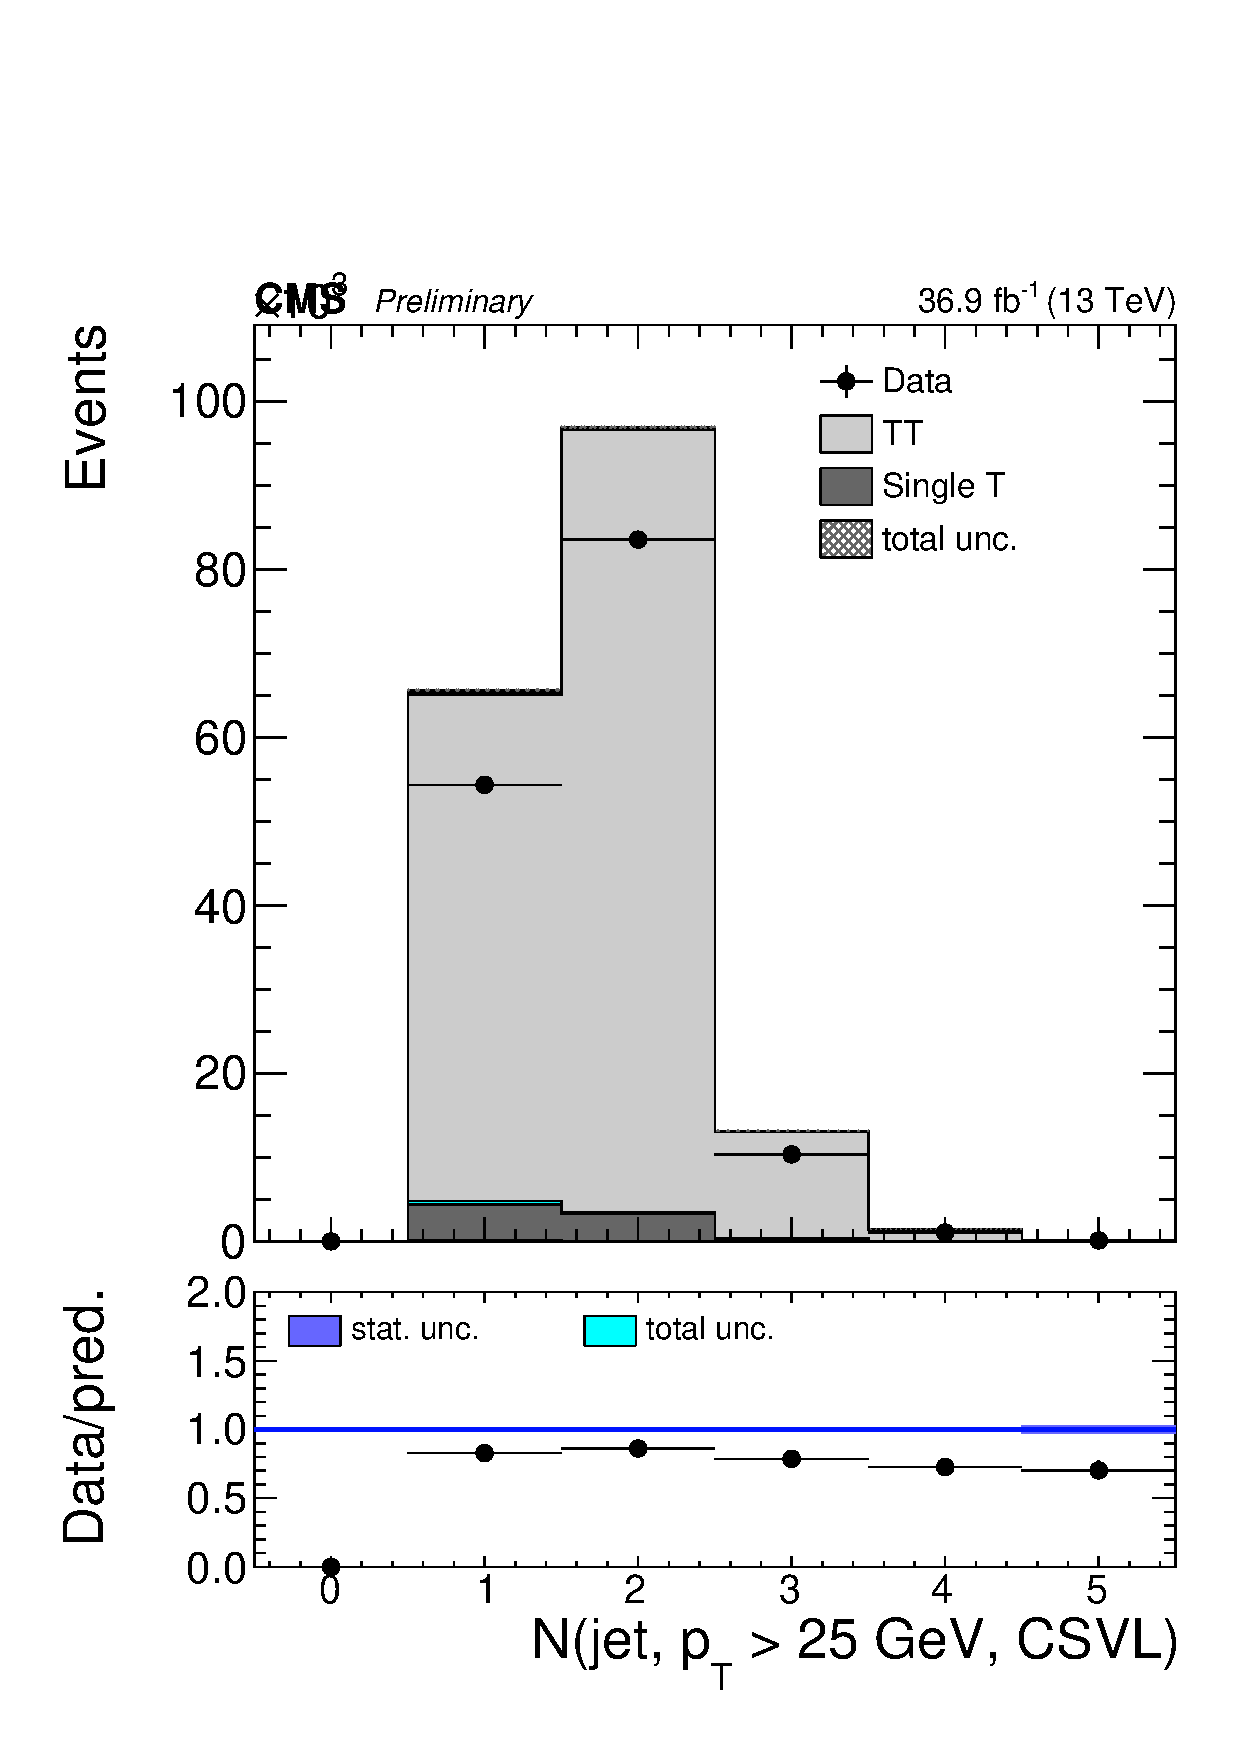
\includegraphics[width=0.35\linewidth]{plots_controlregions/cr_ttbar_data/nBJetLoose25.pdf}\\
%\caption{Data and simulation distributions in the
%$\ttbar\to\Pe^\pm\Pgm^\mp\,\cPqb\cPaqb\,\Pgn\Pagn$ control
%  region. From top left to bottom right: the $E_{T}^{miss}$, the
%$E_{T}^{miss}LD$, the jet multiplicity and the number of jets passing the loose working point of the CSV tagger.
%Uncertainties are statistical only.
%}
%\label{fig:cr_tt2l}
%\end{figure}
%
%\clearpage

%In order to disentangle the mismodeling of jet multiplicity in ttbar MC from the differential description of the other observables, we perform the same study in exclusive bins of jet multiplicity (exactly 2, 3 or 4 jets) and normalize the total yield in the simulation to that observed in data. Figures~\ref{fig:cr_tt2l_jetbins_norm}-\ref{fig:cr_tt2l_jetbins_norm_4j} show a good description of the tested observables (b-jet multiplicity is expected to improve when the dedicated scale factors will be applied).
%
%\begin{figure}[!htb]
%\centering
%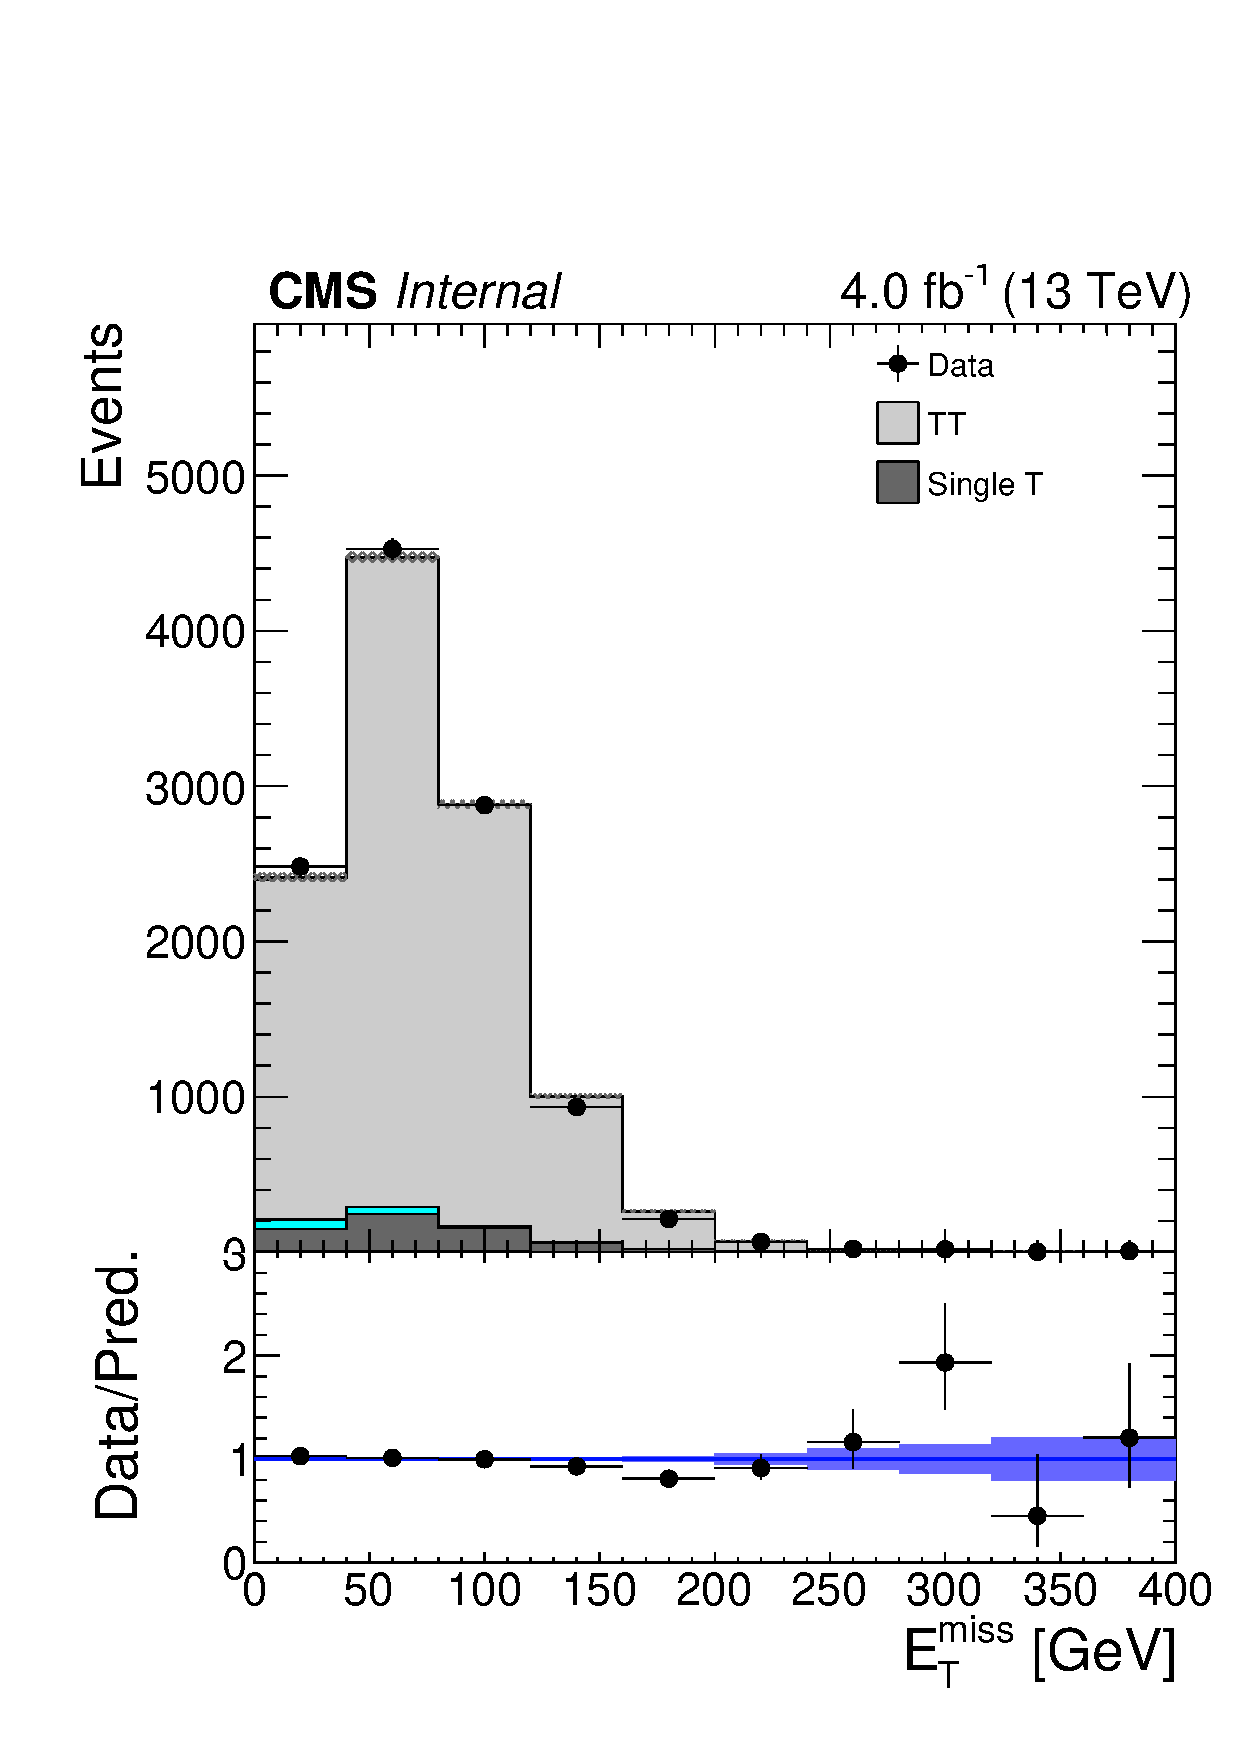
\includegraphics[width=0.32\linewidth]{plots_controlregions/cr_ttbar_data_norm_2j/met.pdf}
%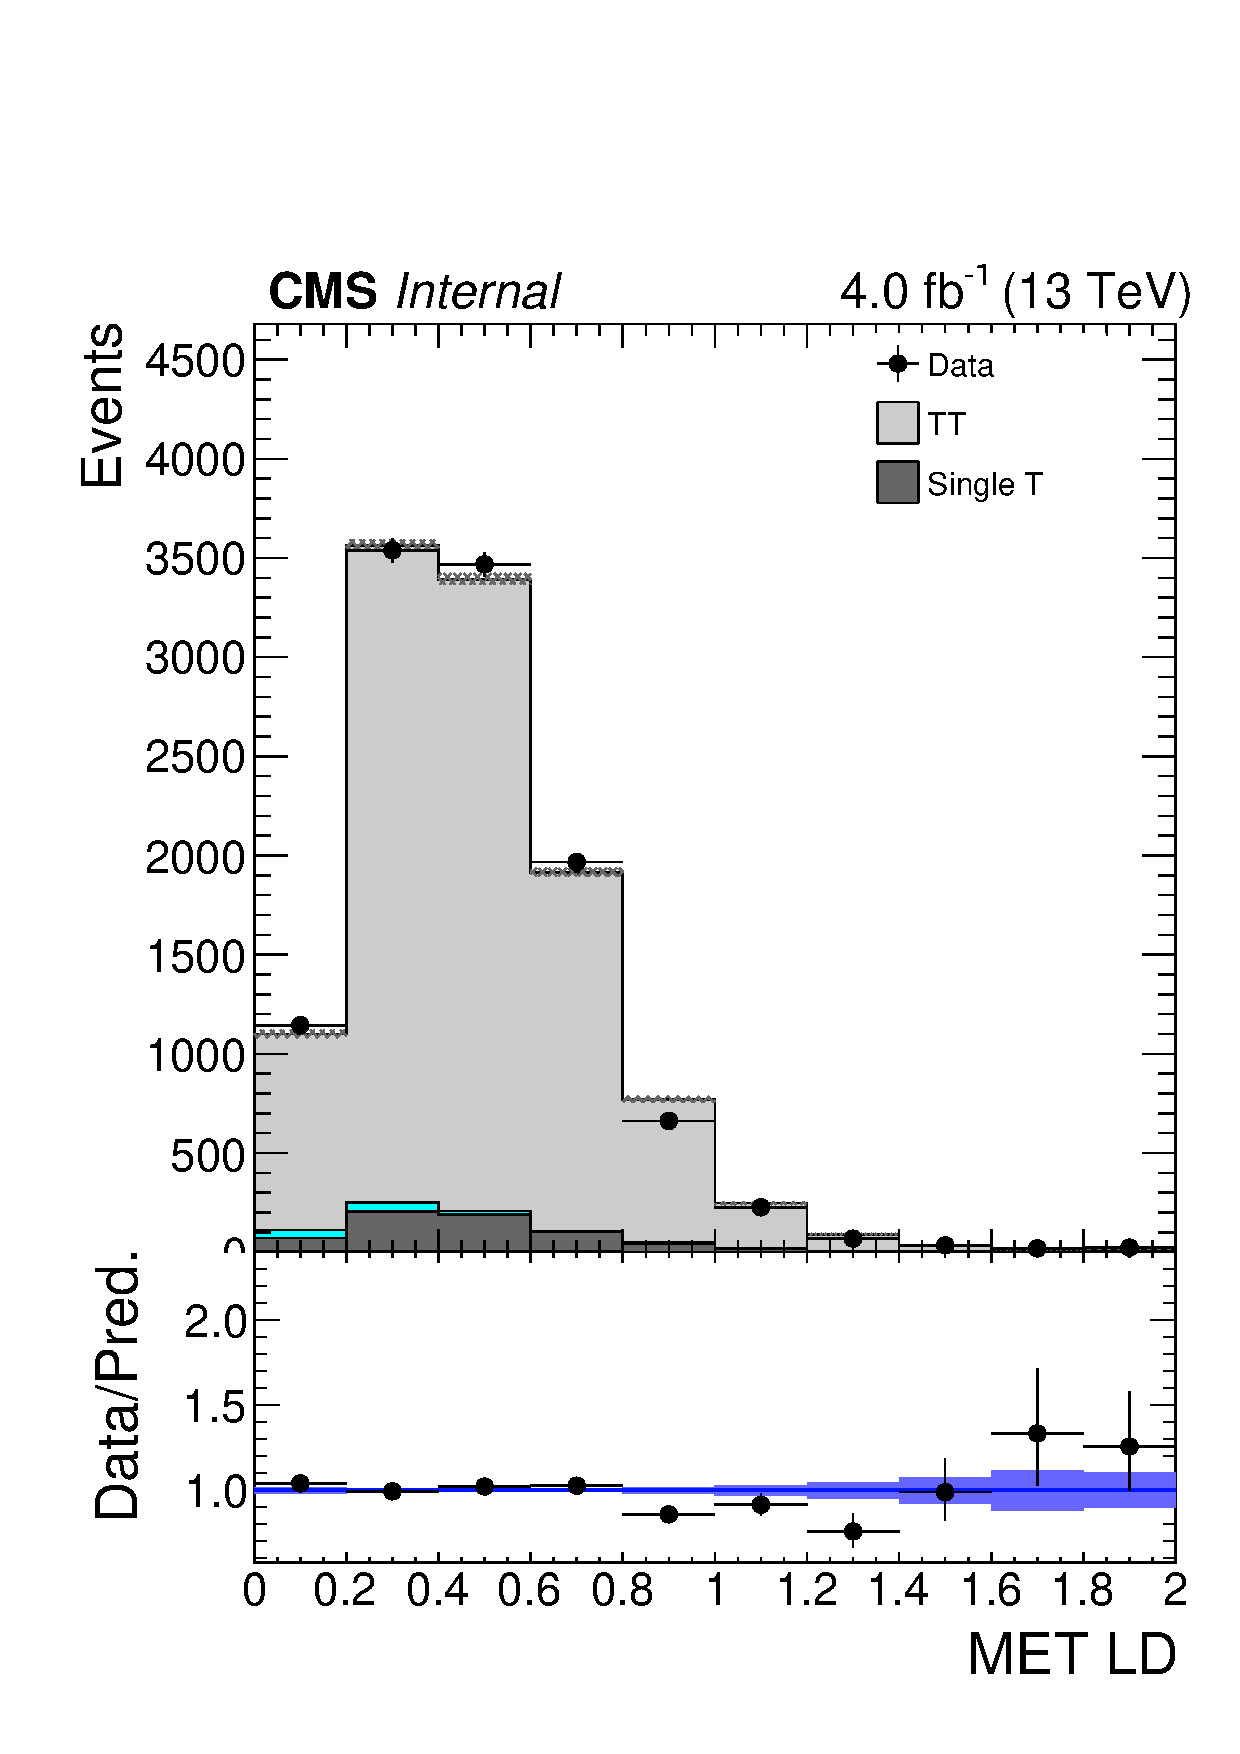
\includegraphics[width=0.32\linewidth]{plots_controlregions/cr_ttbar_data_norm_2j/metLD.pdf}
%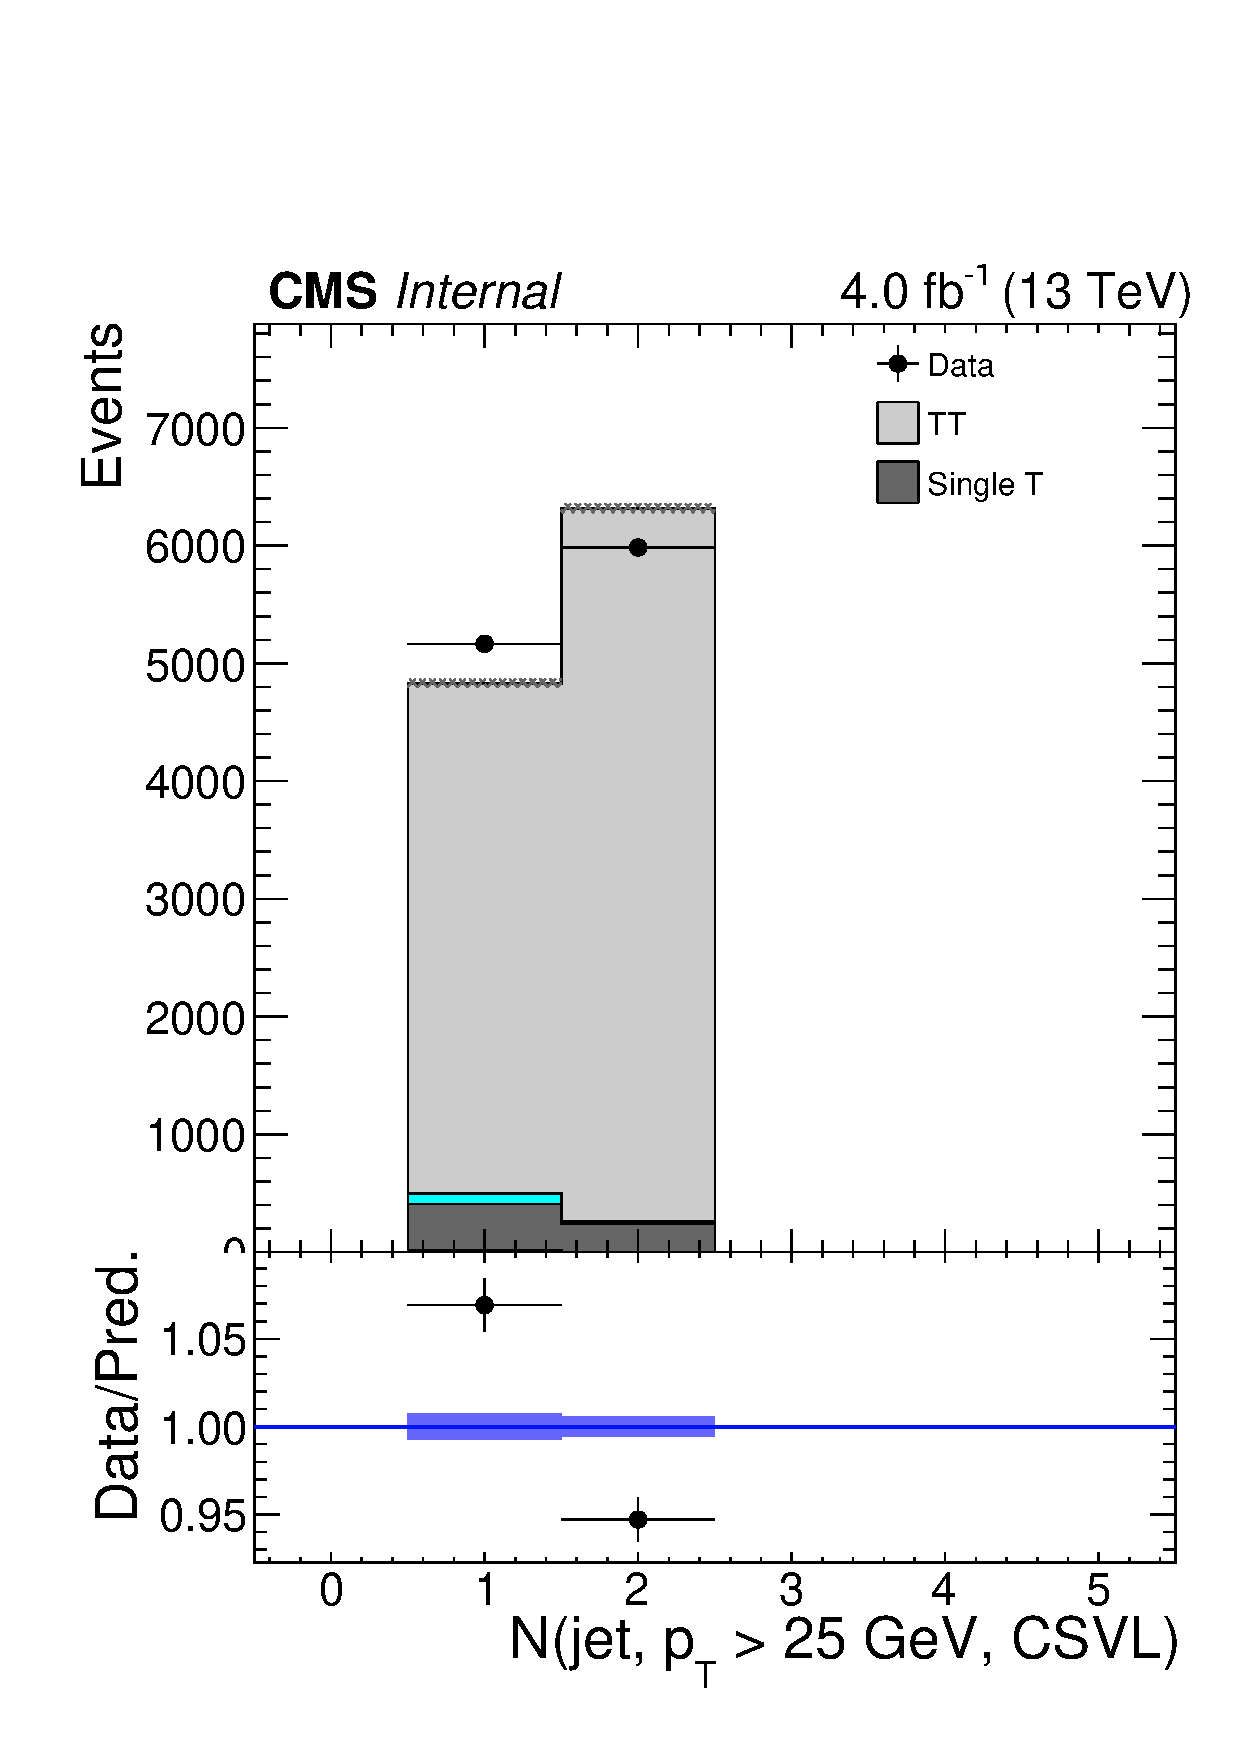
\includegraphics[width=0.32\linewidth]{plots_controlregions/cr_ttbar_data_norm_2j/nBJetLoose25.pdf}\\
%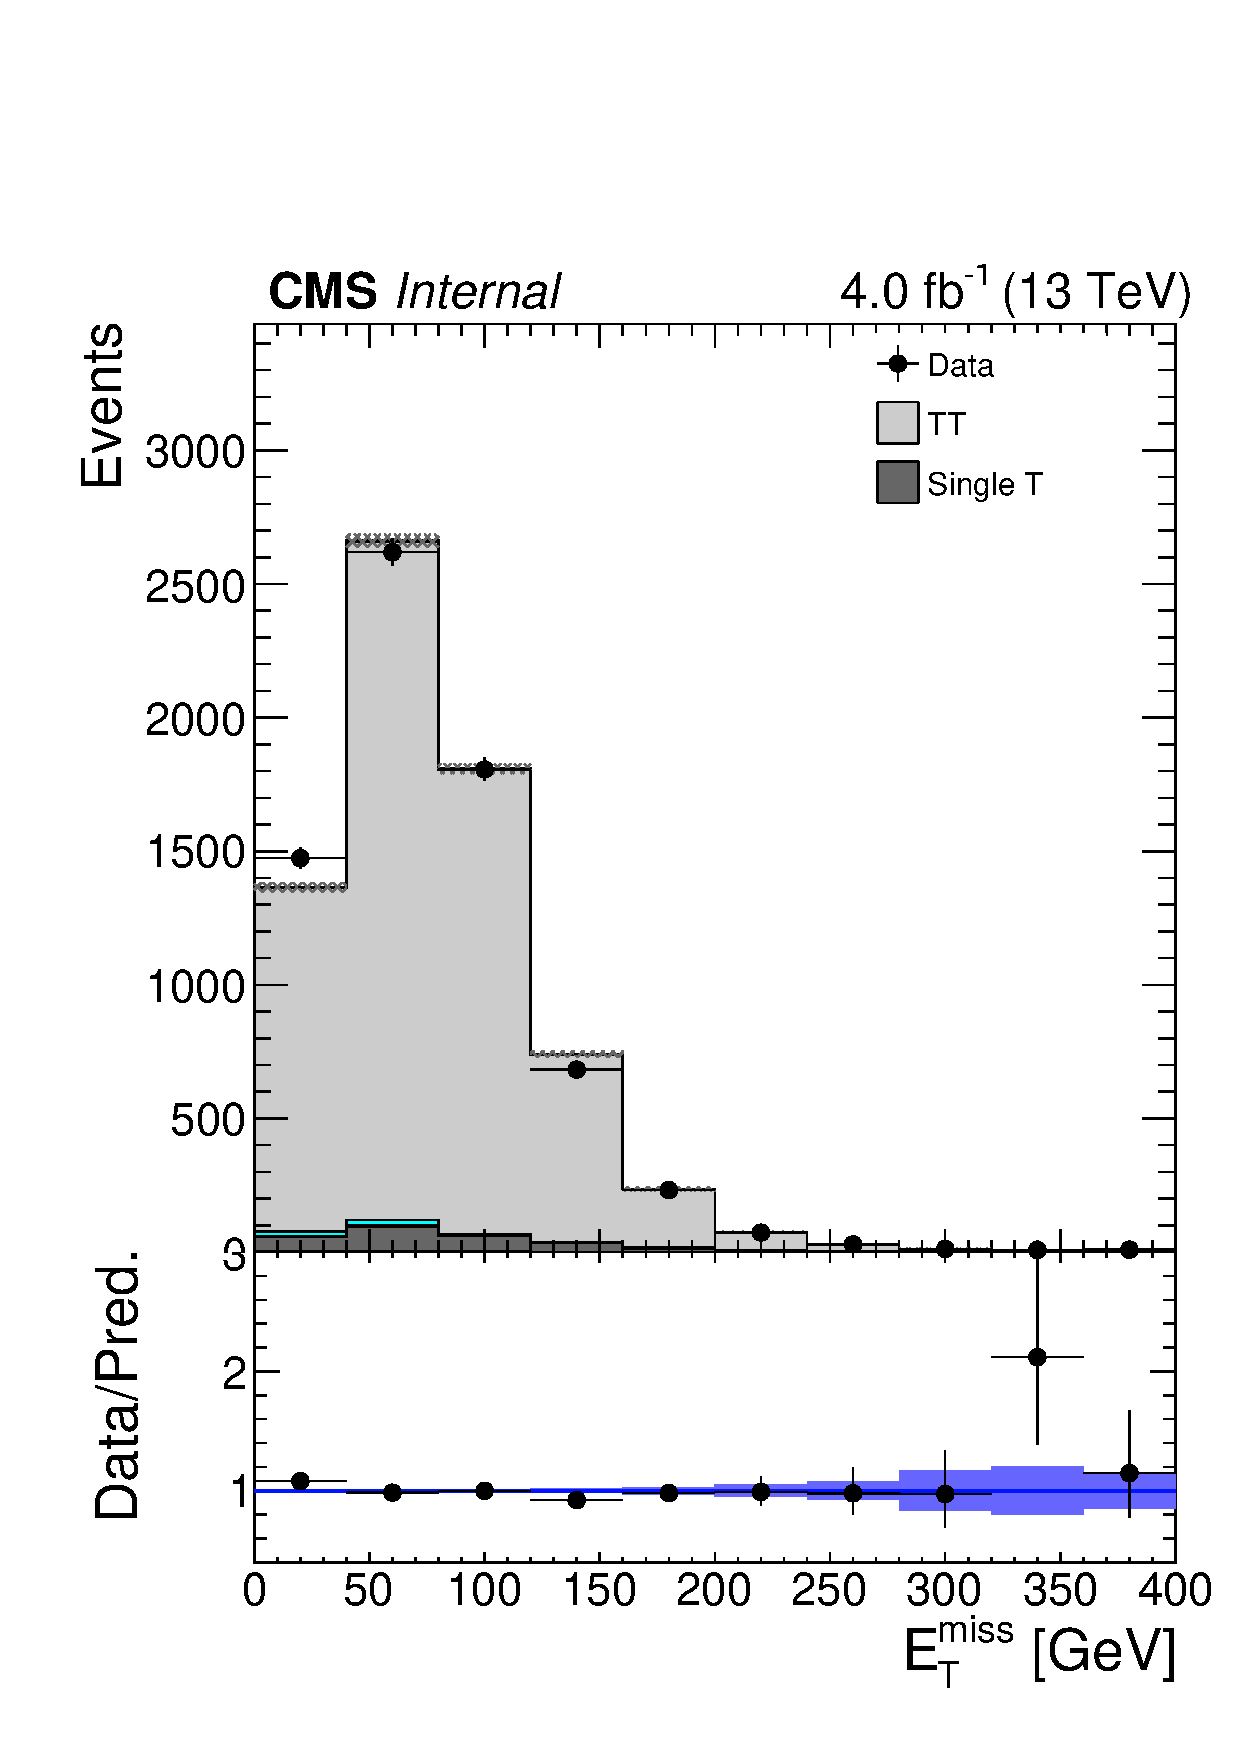
\includegraphics[width=0.32\linewidth]{plots_controlregions/cr_ttbar_data_norm_3j/met.pdf}
%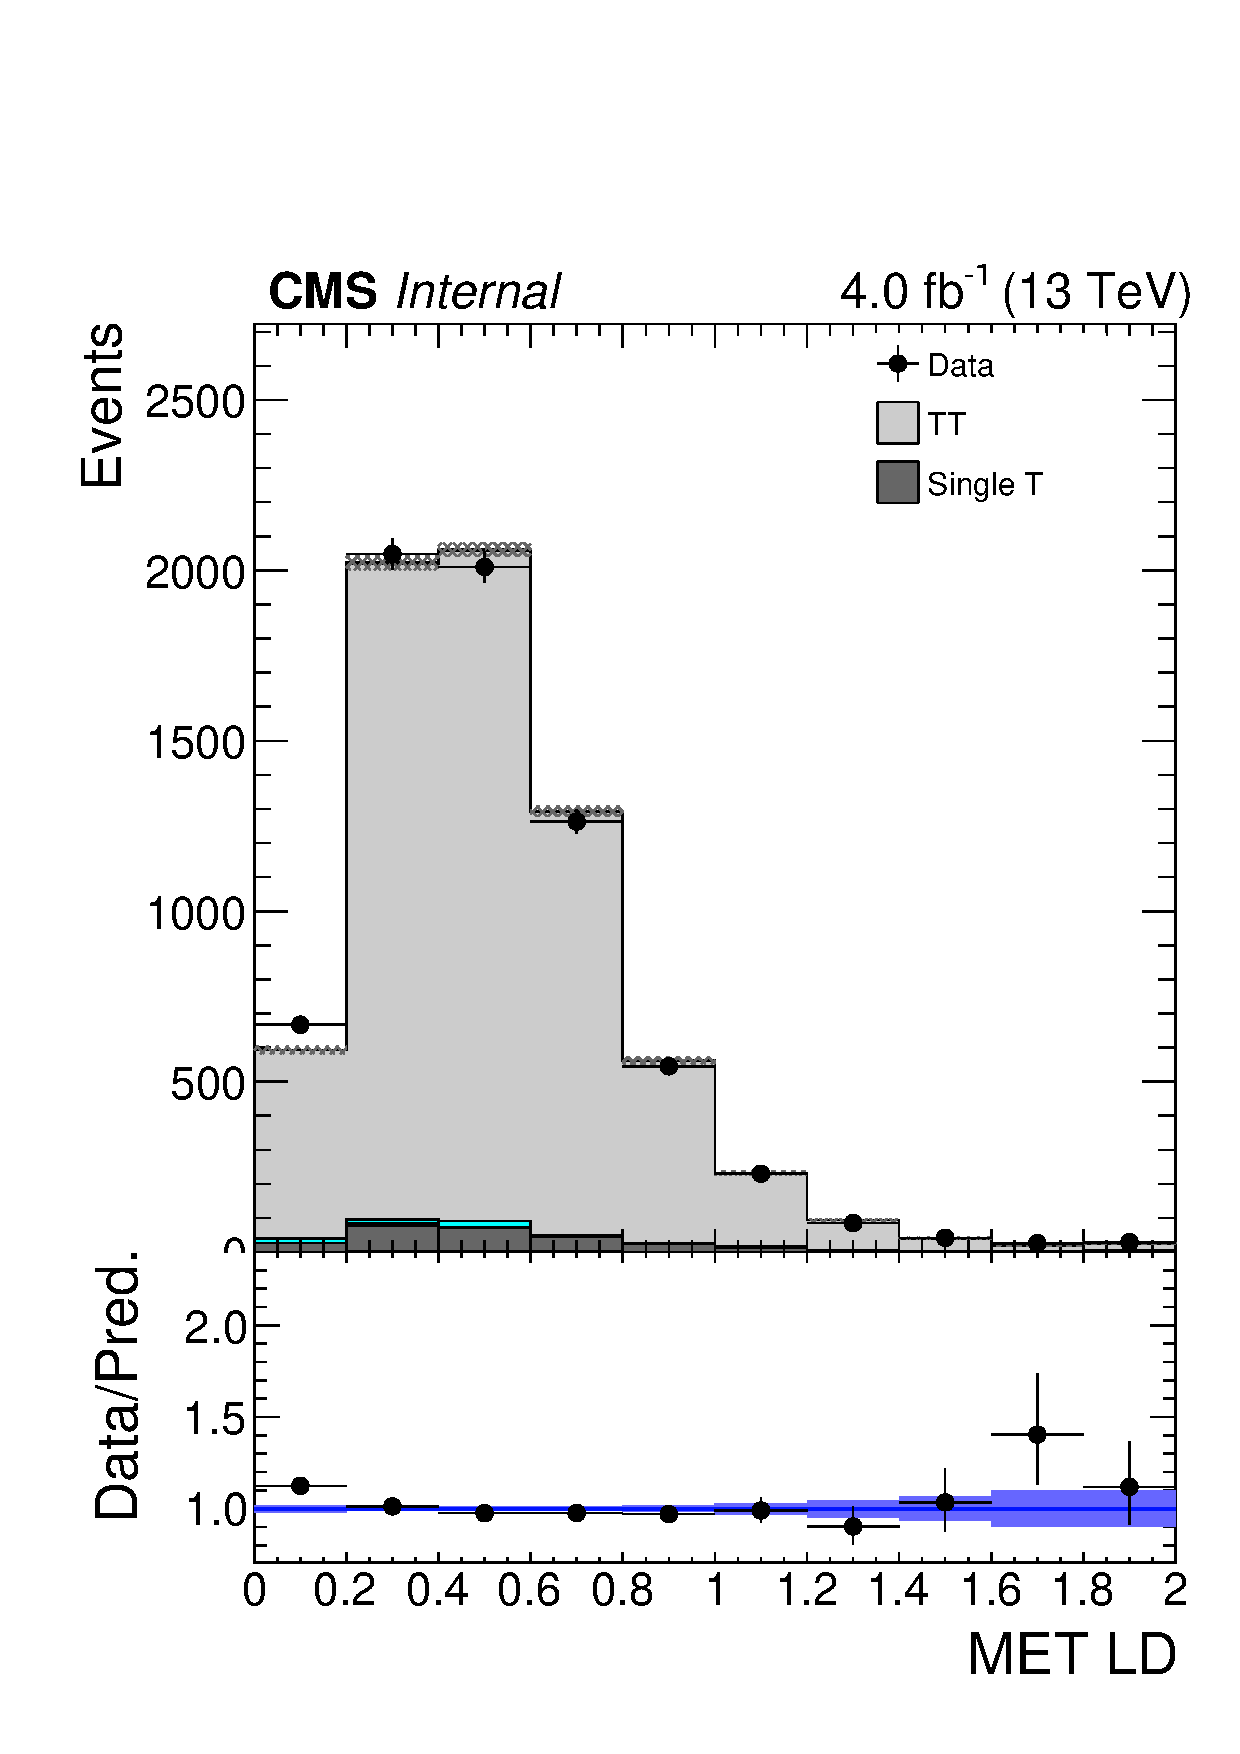
\includegraphics[width=0.32\linewidth]{plots_controlregions/cr_ttbar_data_norm_3j/metLD.pdf}
%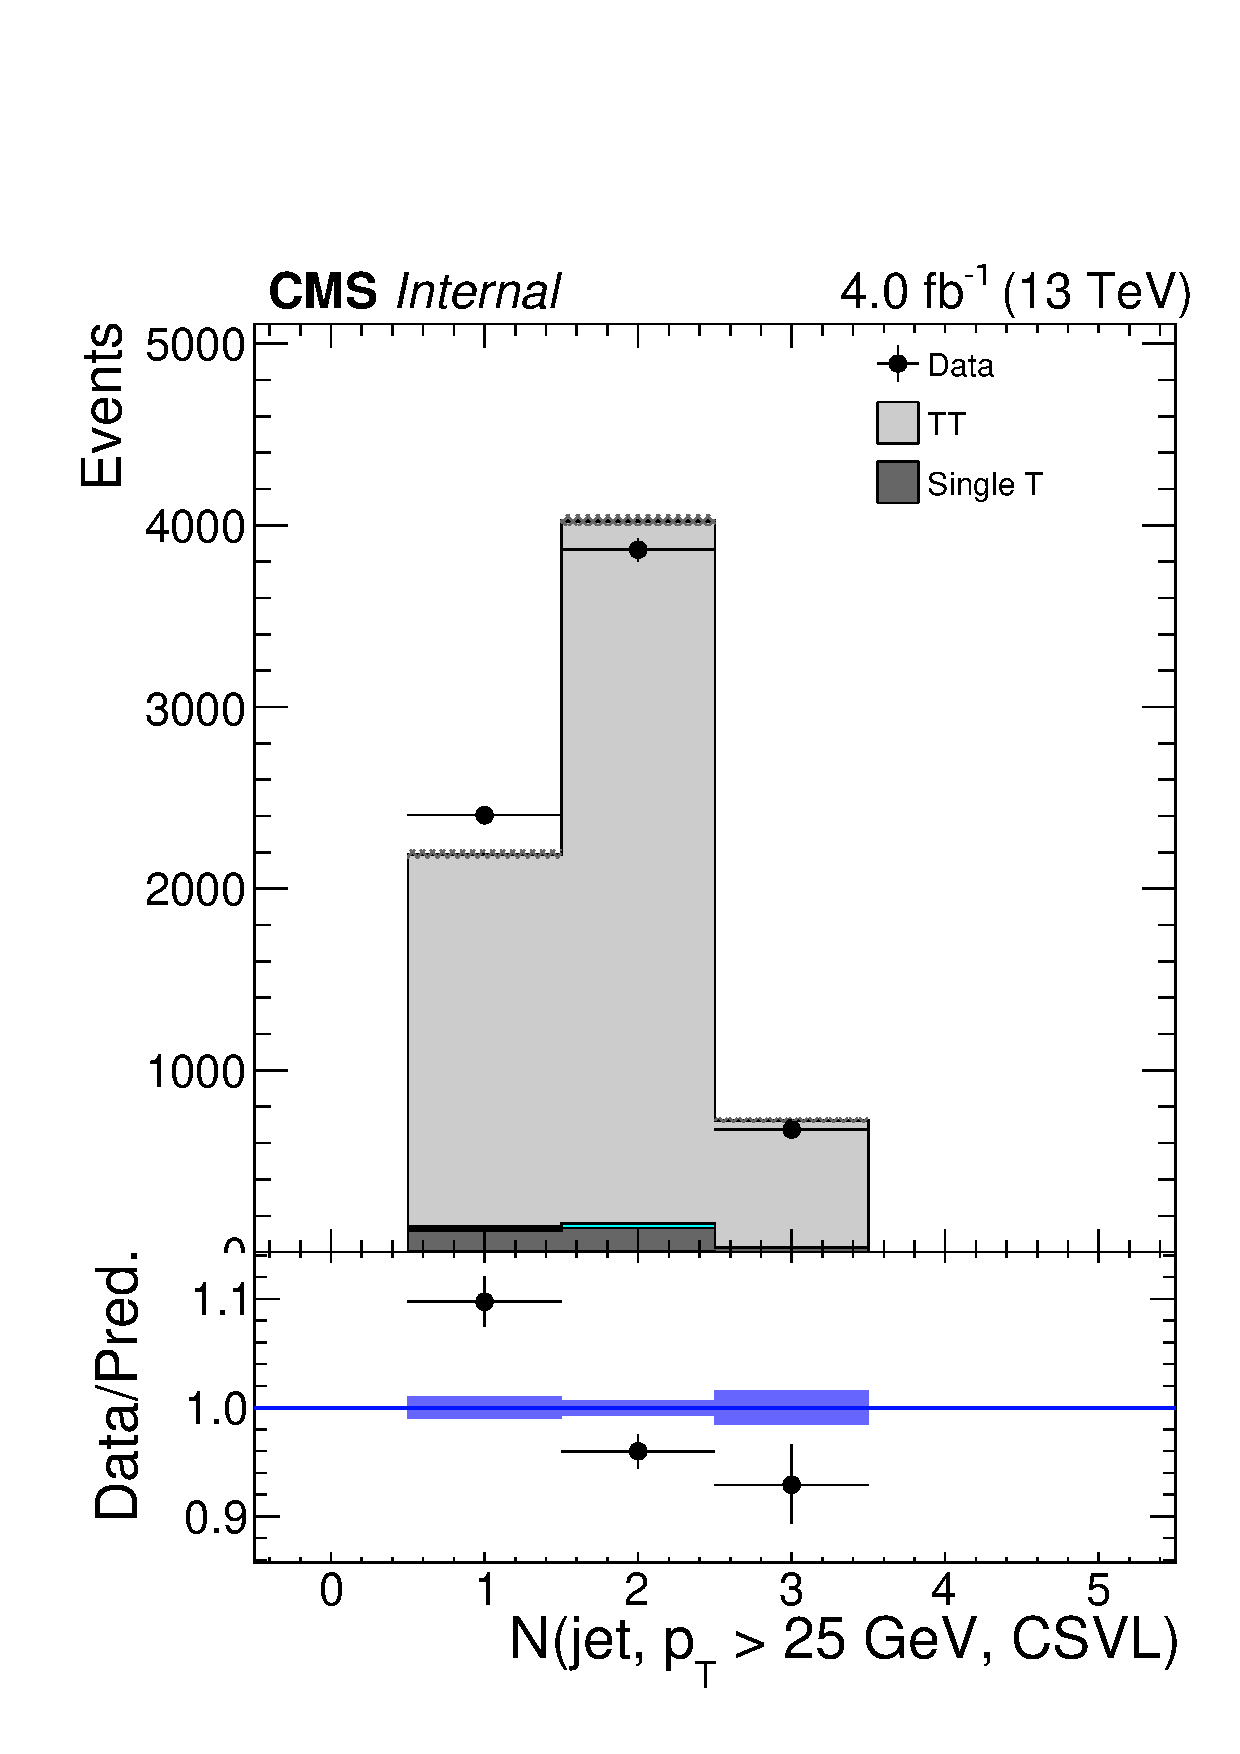
\includegraphics[width=0.32\linewidth]{plots_controlregions/cr_ttbar_data_norm_3j/nBJetLoose25.pdf}\\
%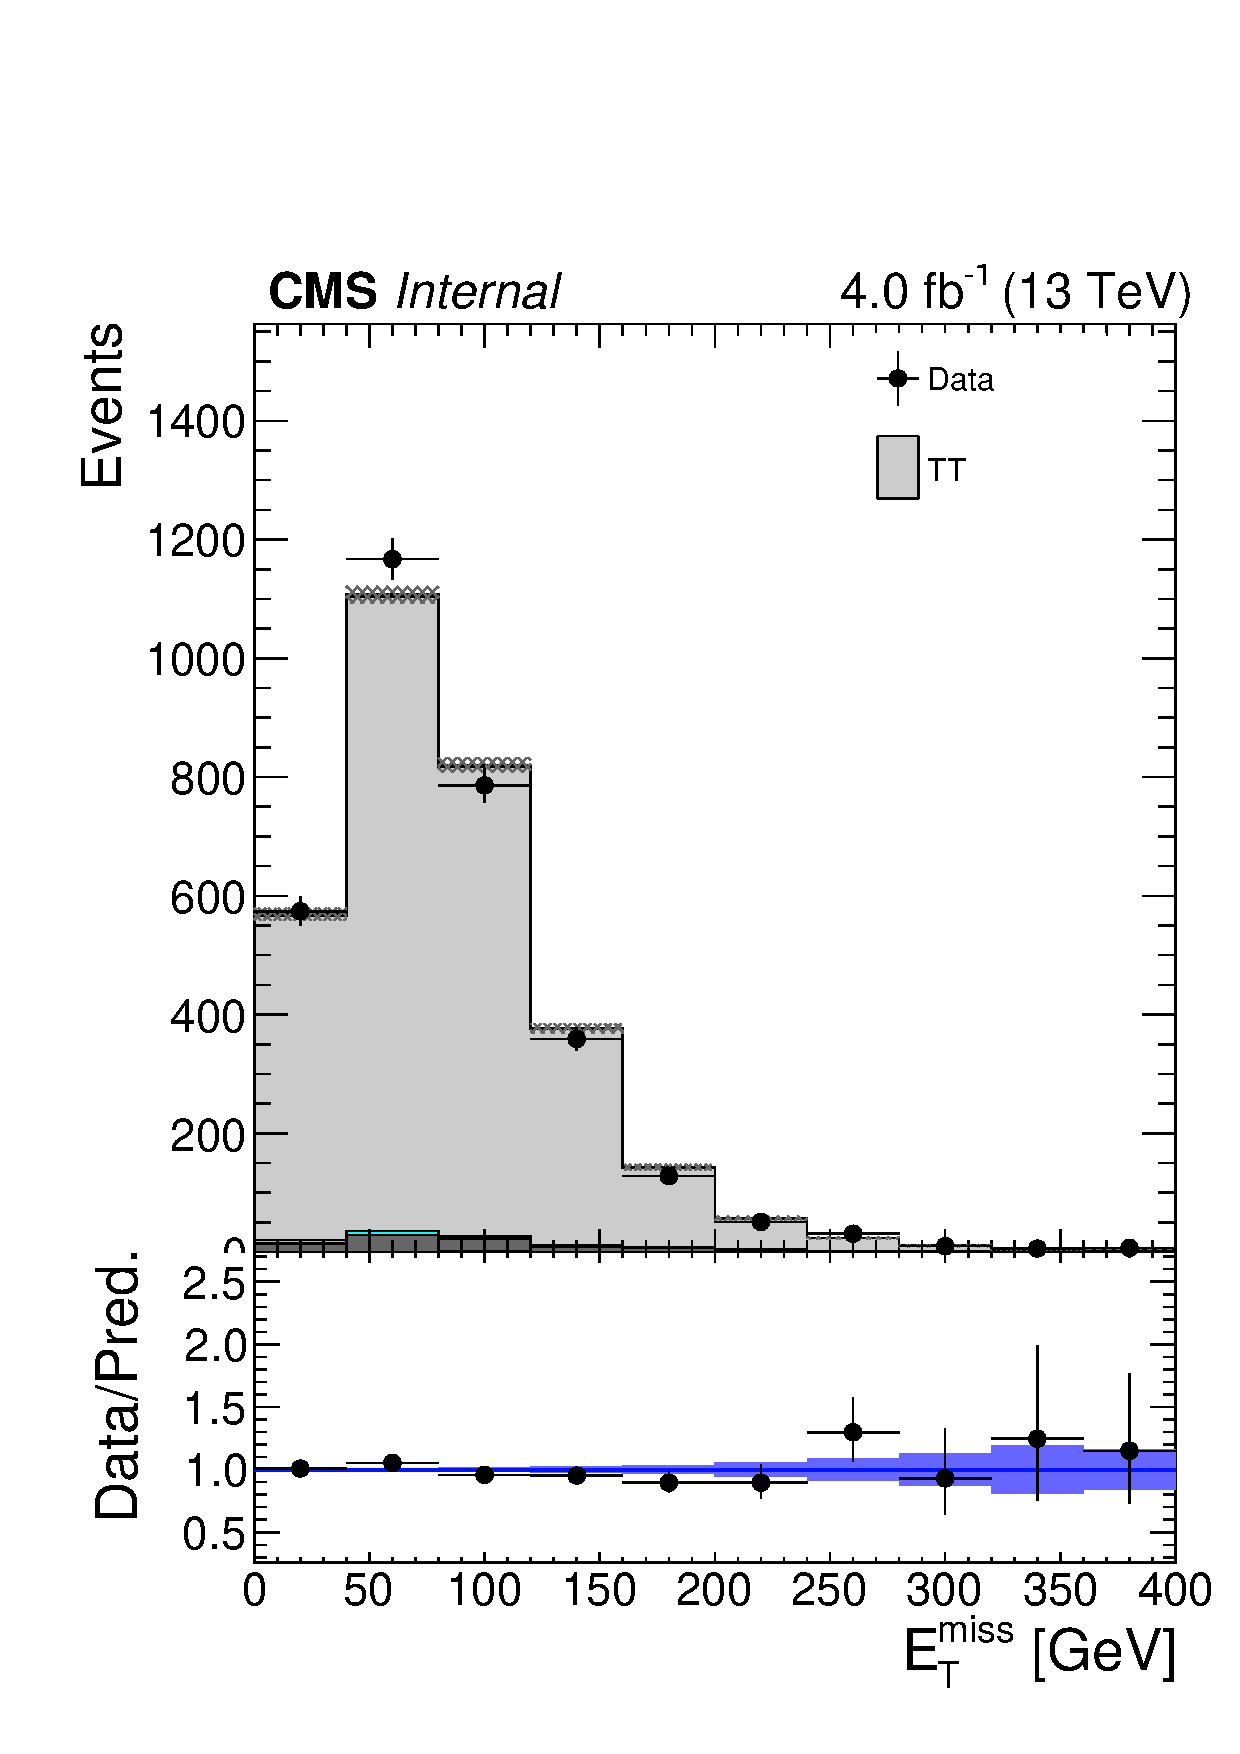
\includegraphics[width=0.32\linewidth]{plots_controlregions/cr_ttbar_data_norm_4j/met.pdf}
%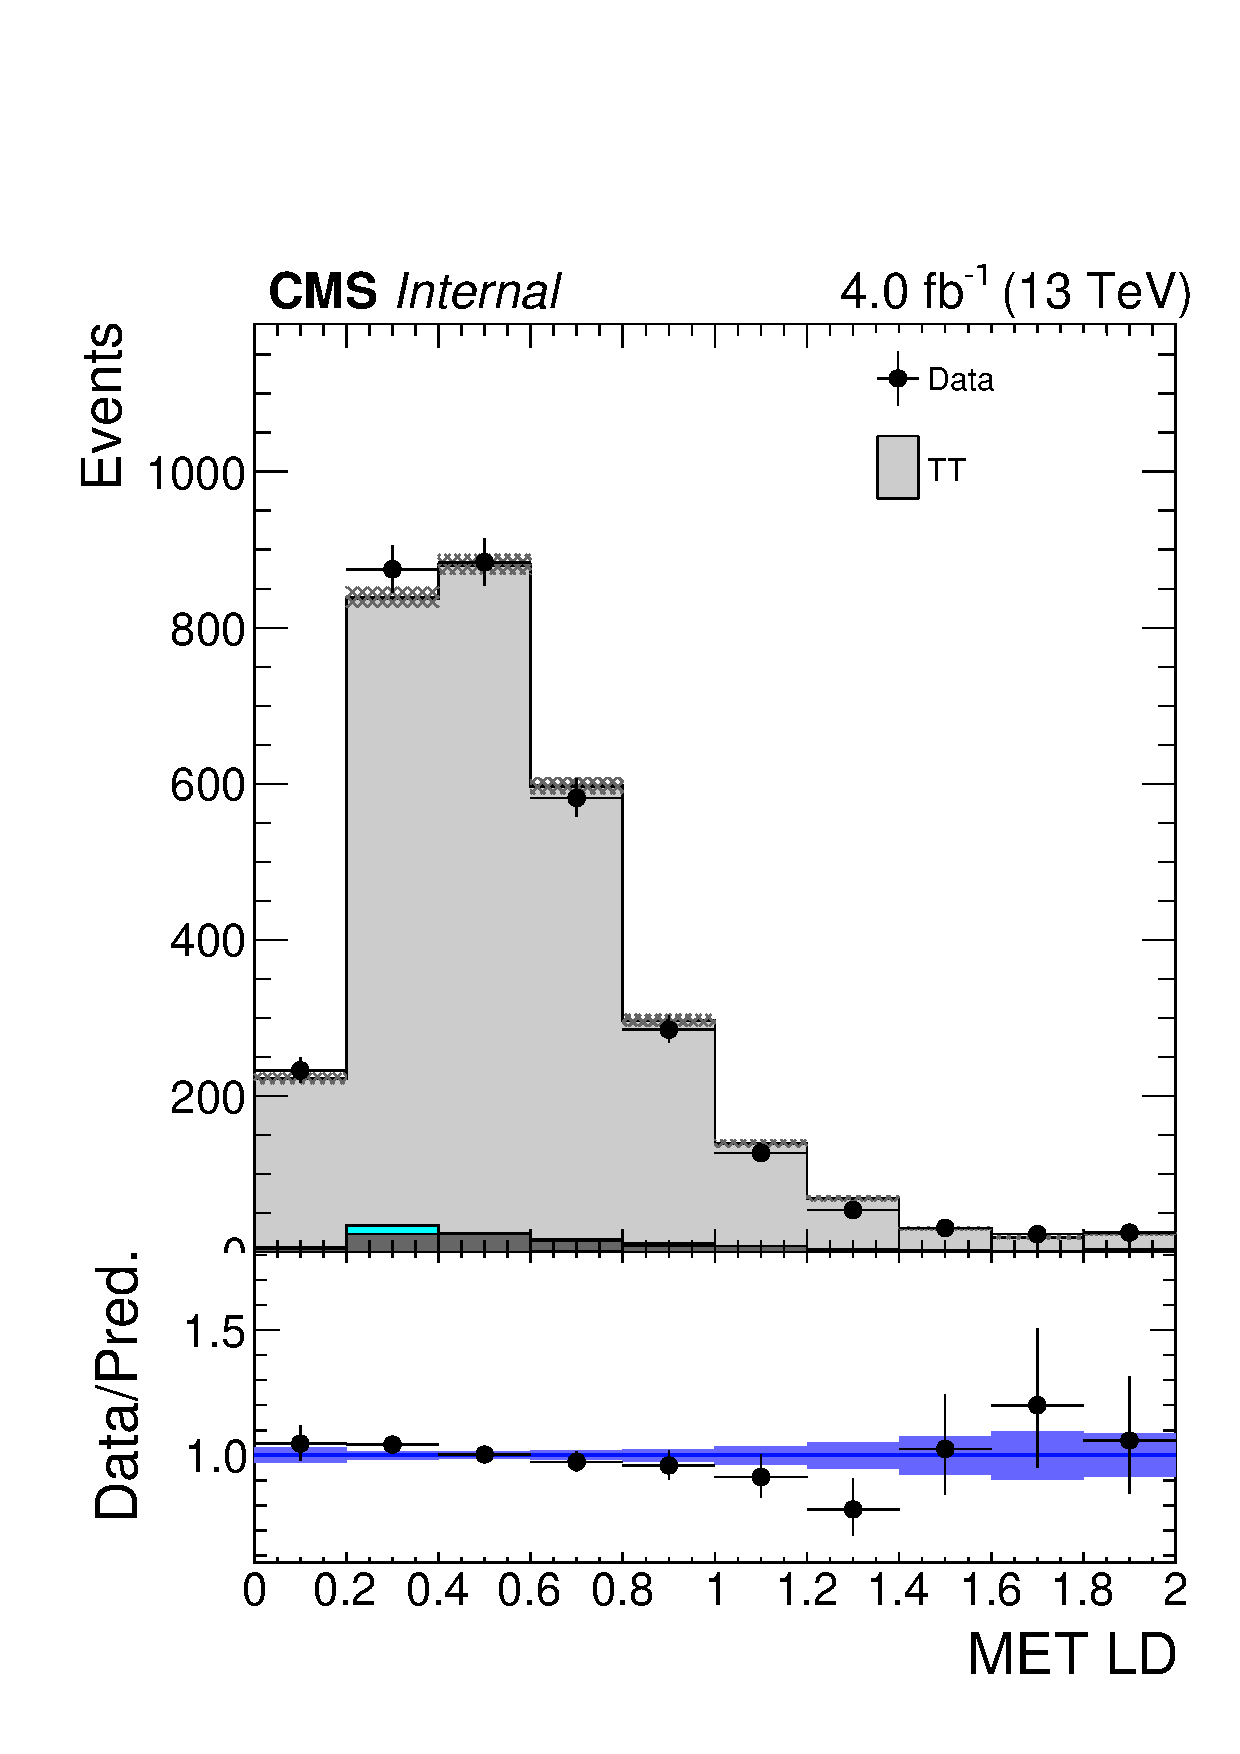
\includegraphics[width=0.32\linewidth]{plots_controlregions/cr_ttbar_data_norm_4j/metLD.pdf}
%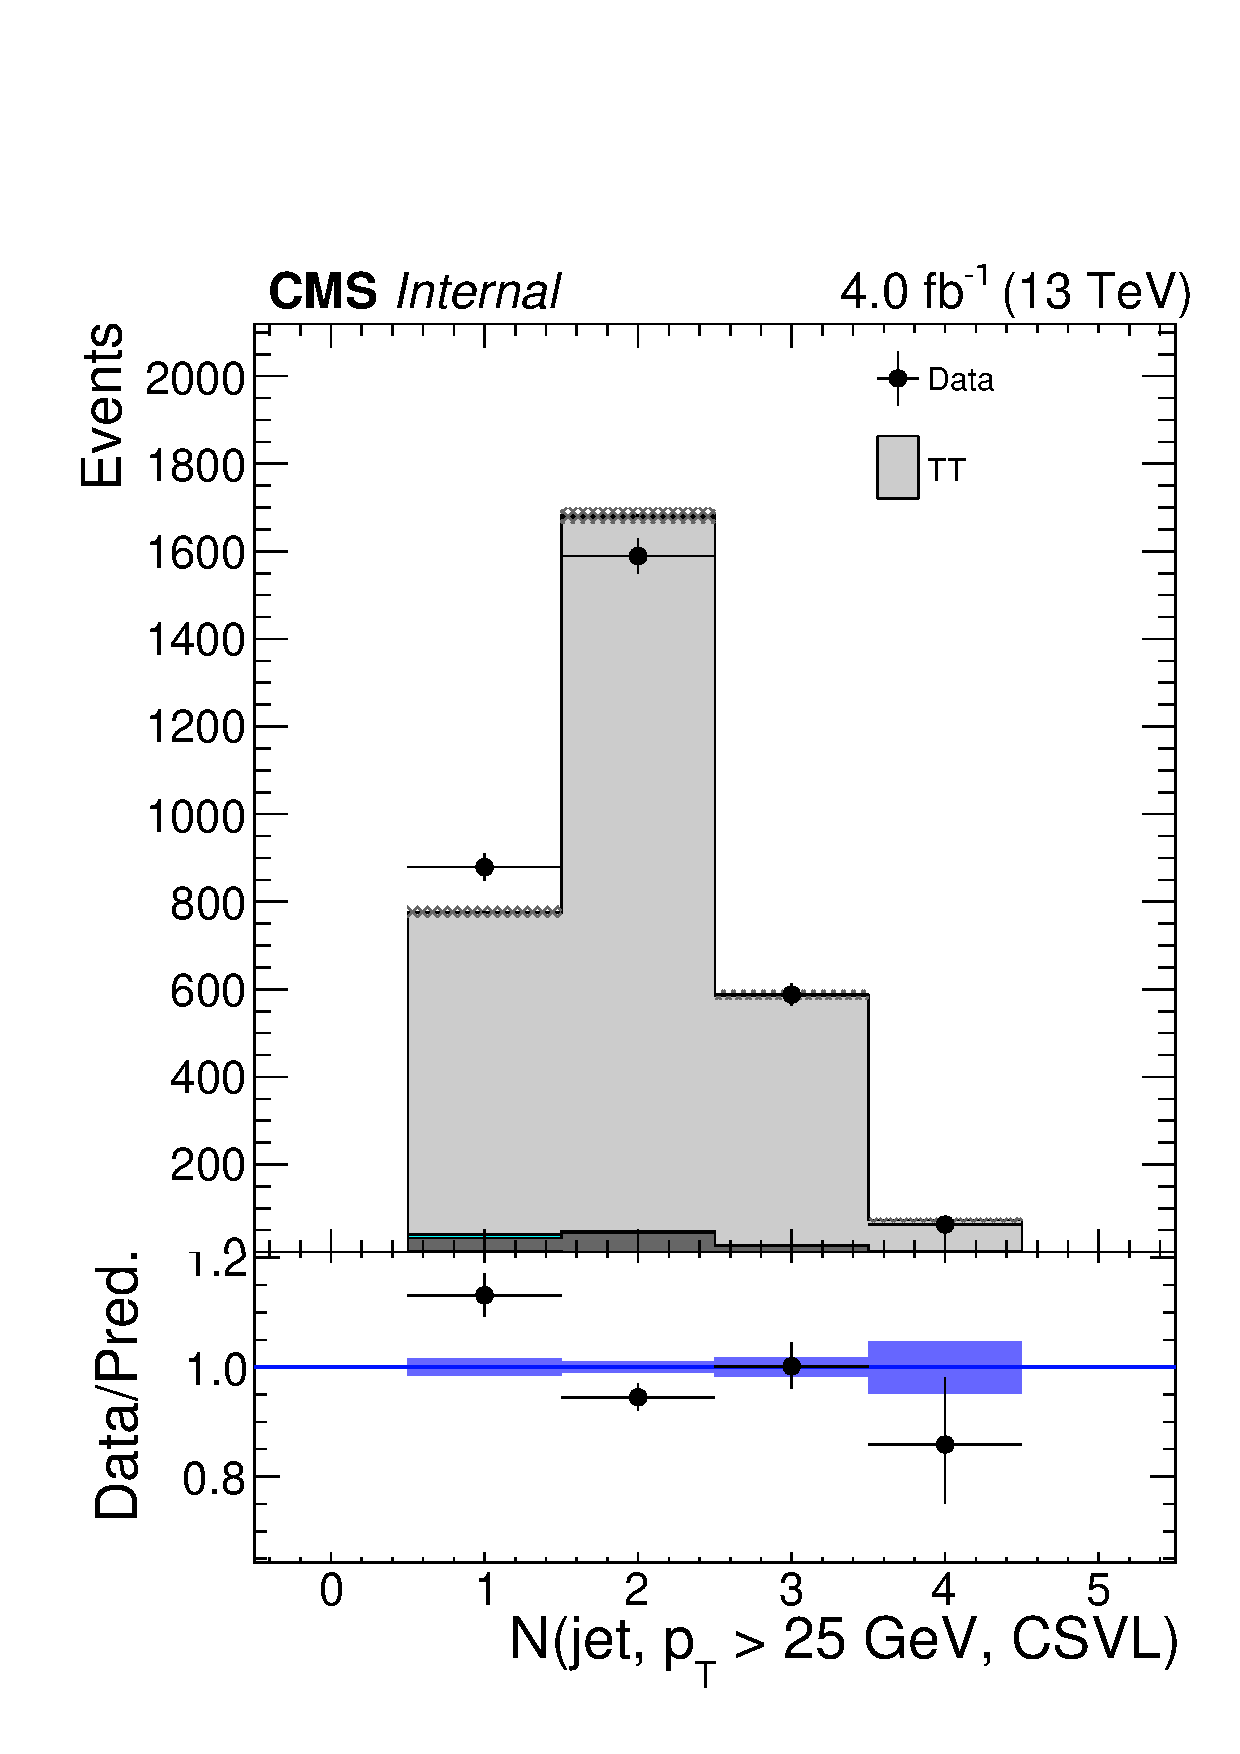
\includegraphics[width=0.32\linewidth]{plots_controlregions/cr_ttbar_data_norm_4j/nBJetLoose25.pdf}\\
%\caption{Data and simulation distributions in the
%$\ttbar\to\Pe^\pm\Pgm^\mp\,\cPqb\cPaqb\,\Pgn\Pagn$ control
%  region, with exactly 2 jets (top row), 3 jets (central row) and 4 jets (bottom row) in the final state. Simulation is normalized to data. Uncertainties are statistical only. B-tag scale factors are not applied.
%}
%\label{fig:cr_tt2l_jetbins_norm}
%\end{figure}
%
%\begin{figure}[!htb]
%\centering
%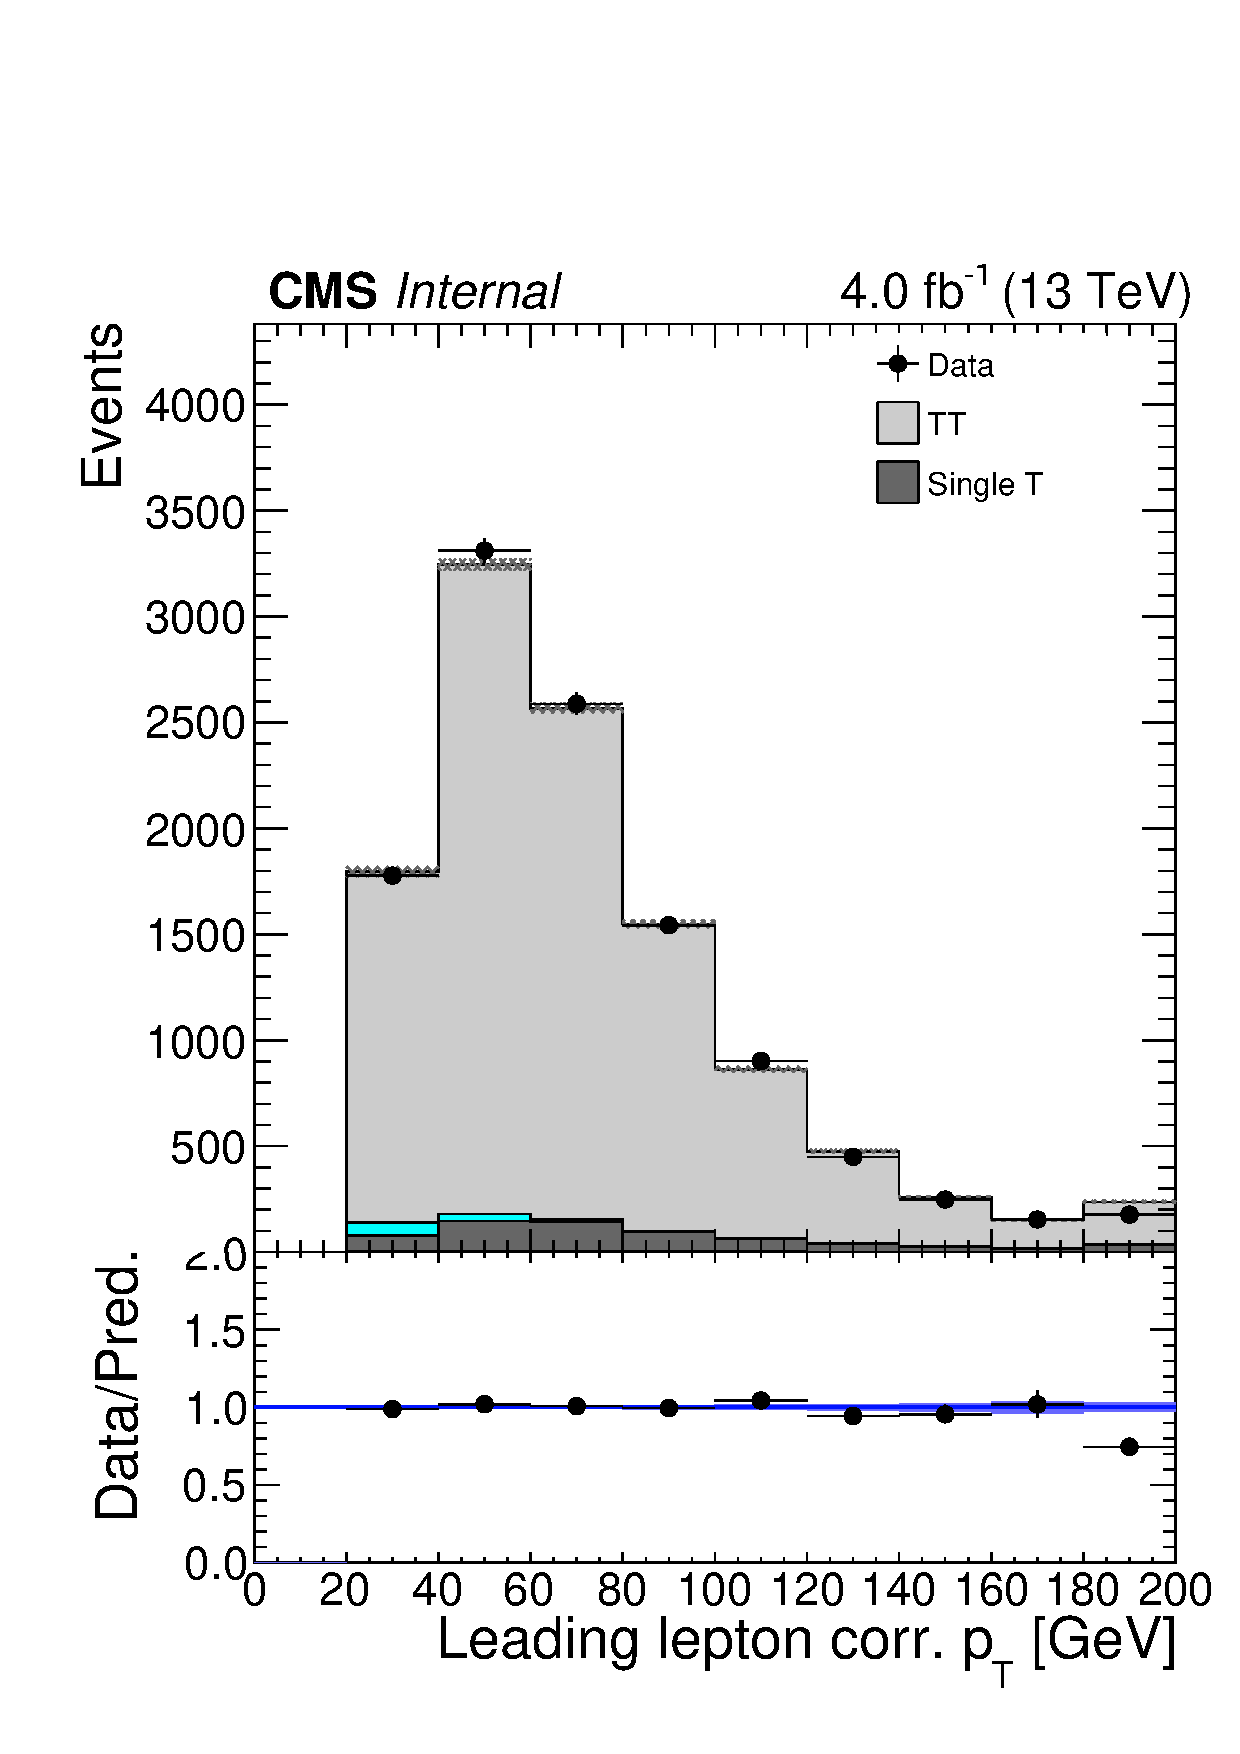
\includegraphics[width=0.32\linewidth]{plots_controlregions/cr_ttbar_data_norm_2j/kinMVA_input_LepGood0_conePt.pdf}
%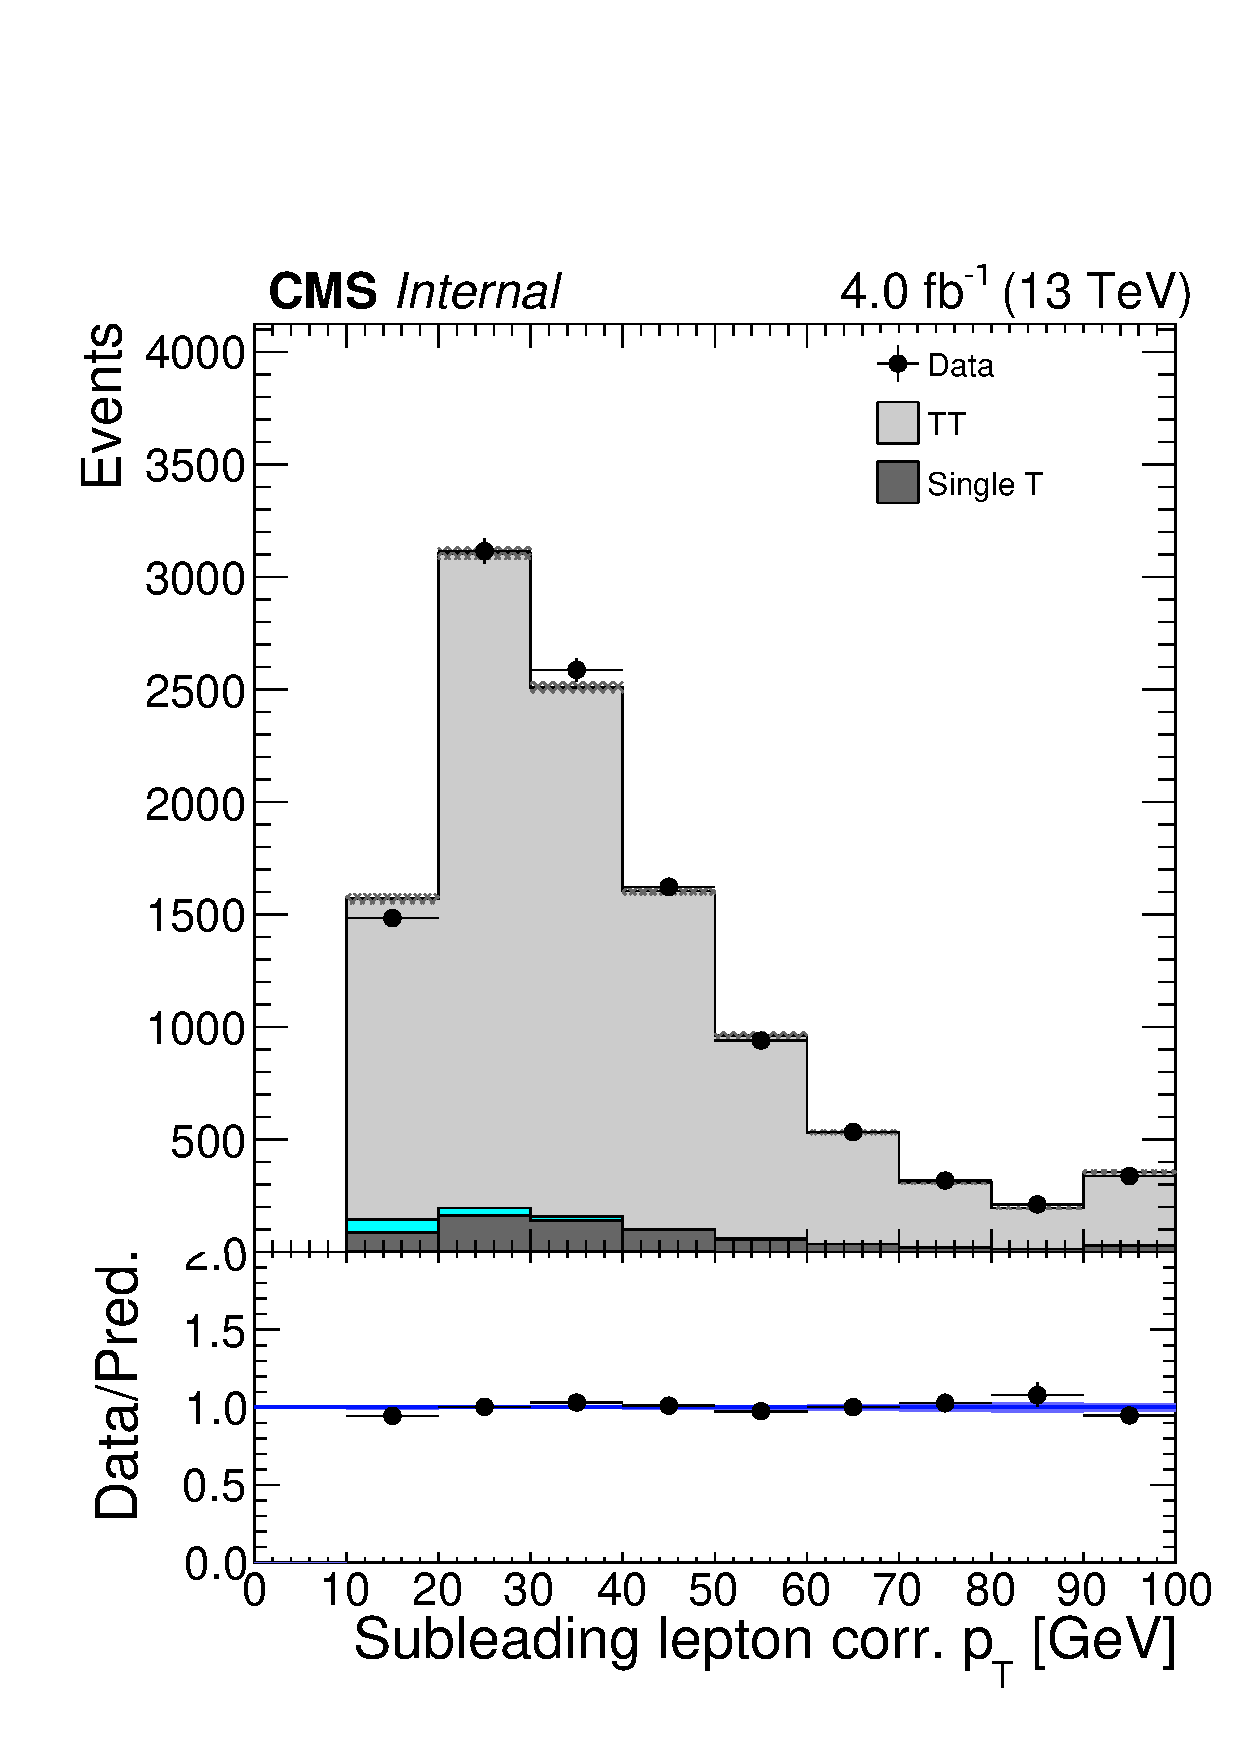
\includegraphics[width=0.32\linewidth]{plots_controlregions/cr_ttbar_data_norm_2j/kinMVA_input_LepGood1_conePt.pdf}
%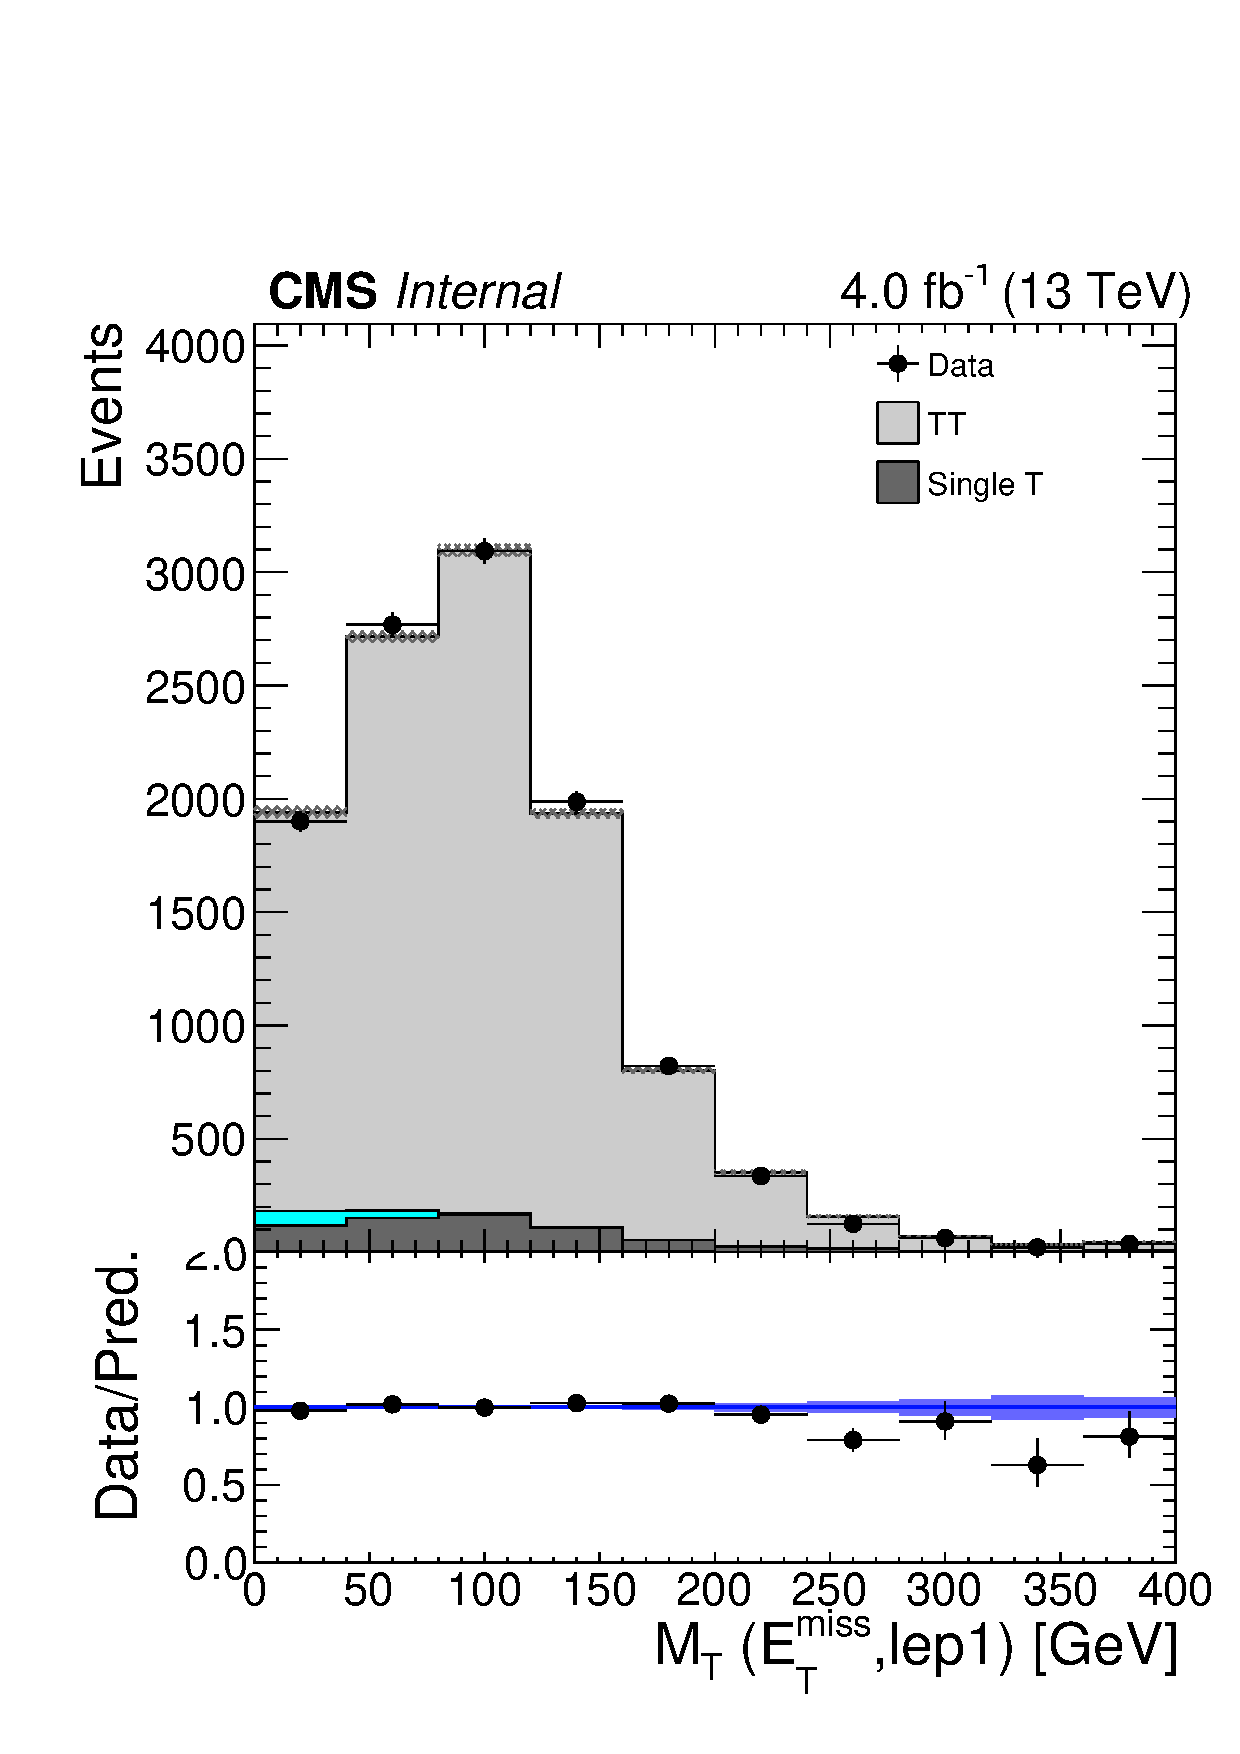
\includegraphics[width=0.32\linewidth]{plots_controlregions/cr_ttbar_data_norm_2j/kinMVA_input_MT_met_lep1.pdf}\\
%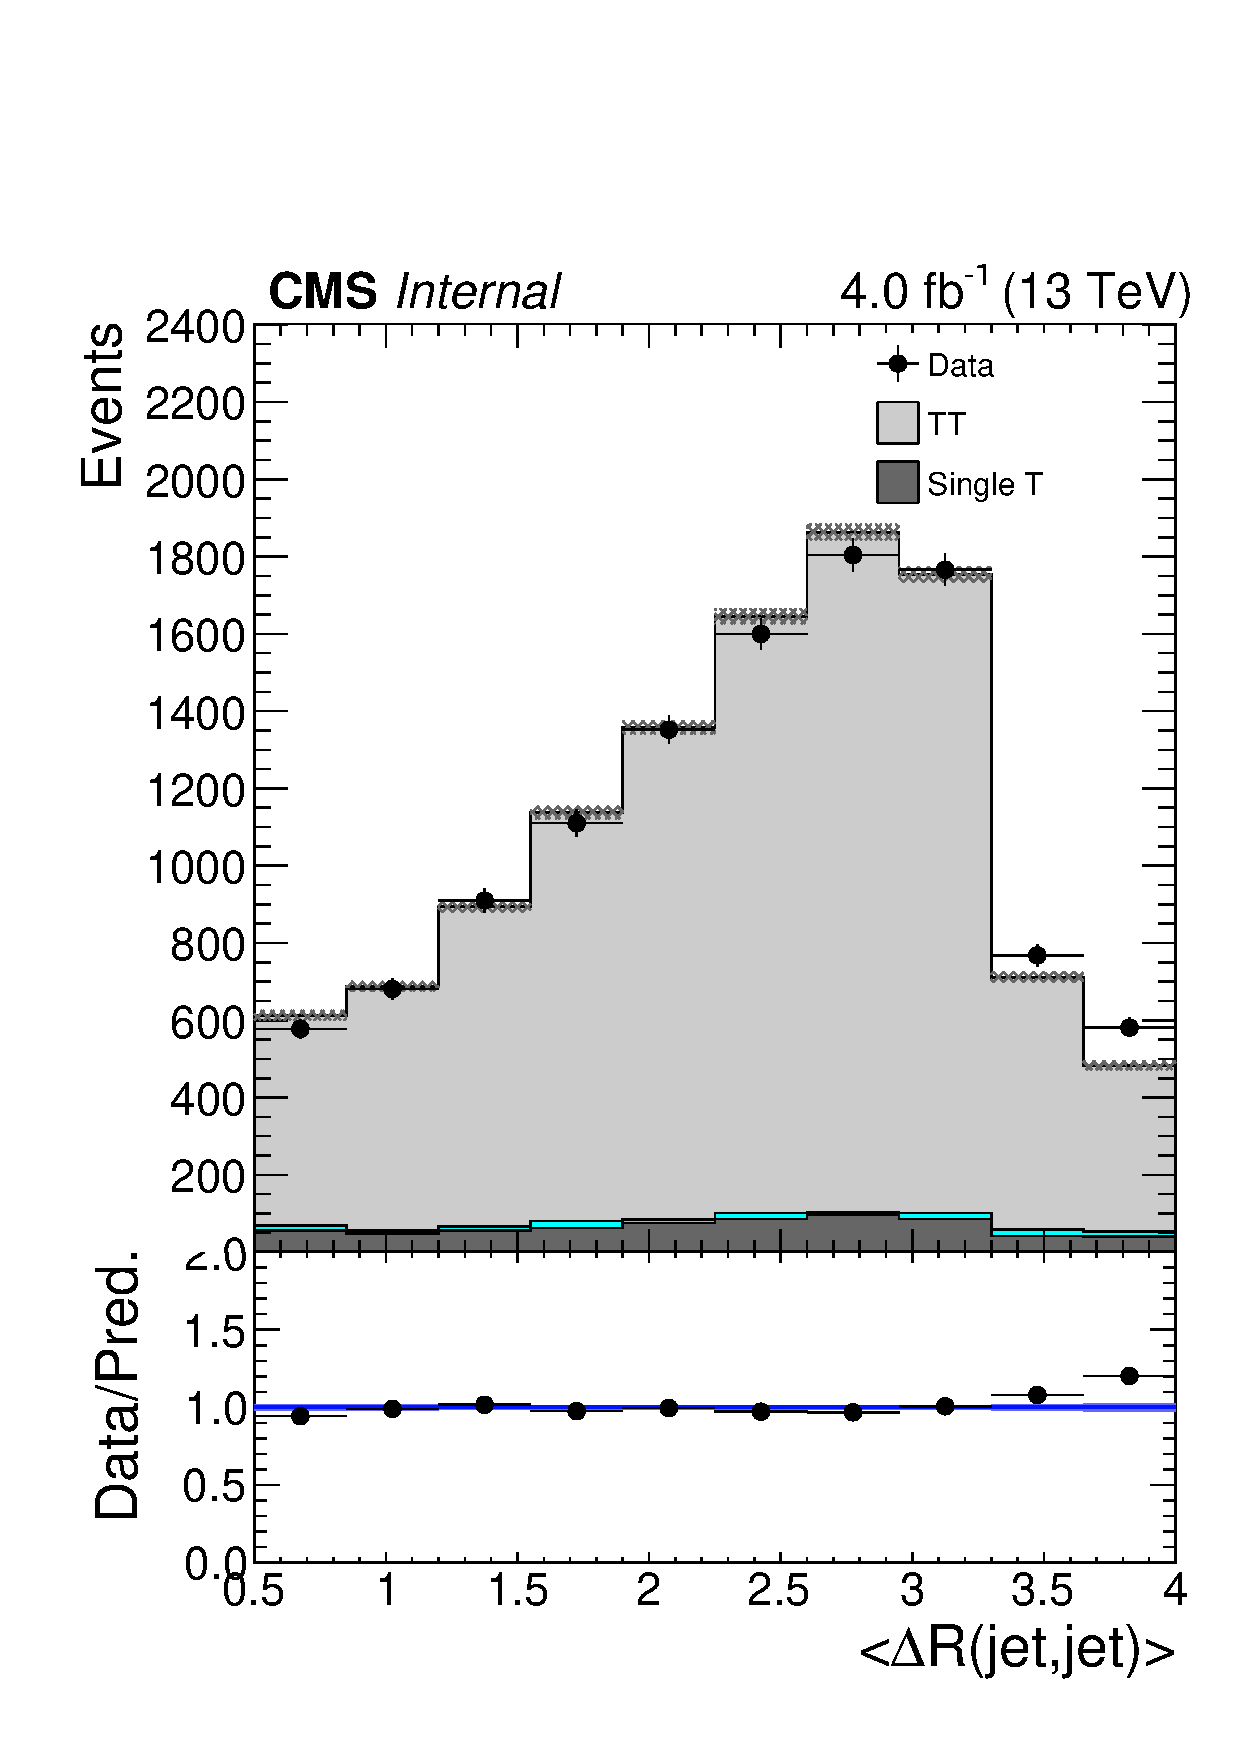
\includegraphics[width=0.32\linewidth]{plots_controlregions/cr_ttbar_data_norm_2j/kinMVA_input_avg_dr_jet.pdf}
%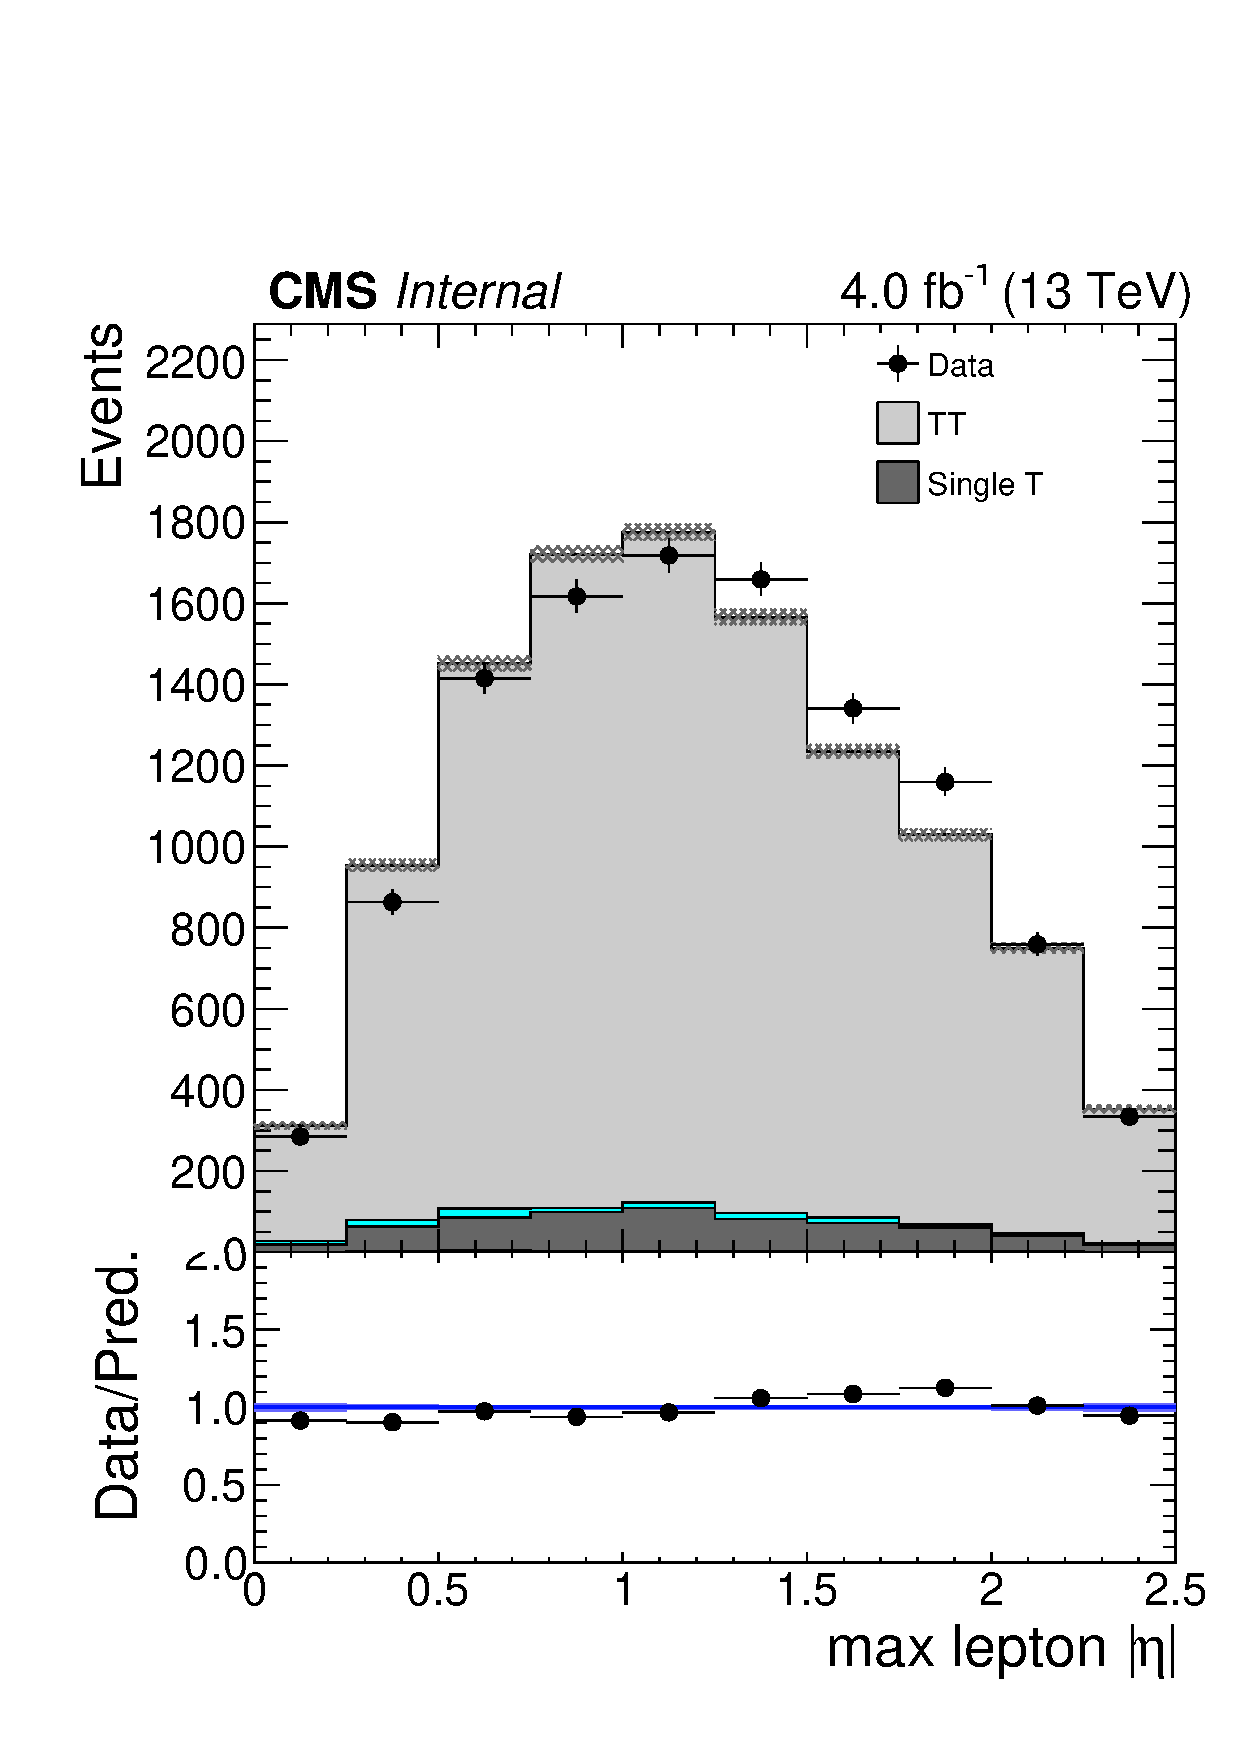
\includegraphics[width=0.32\linewidth]{plots_controlregions/cr_ttbar_data_norm_2j/kinMVA_input_max_Lep_eta.pdf}
%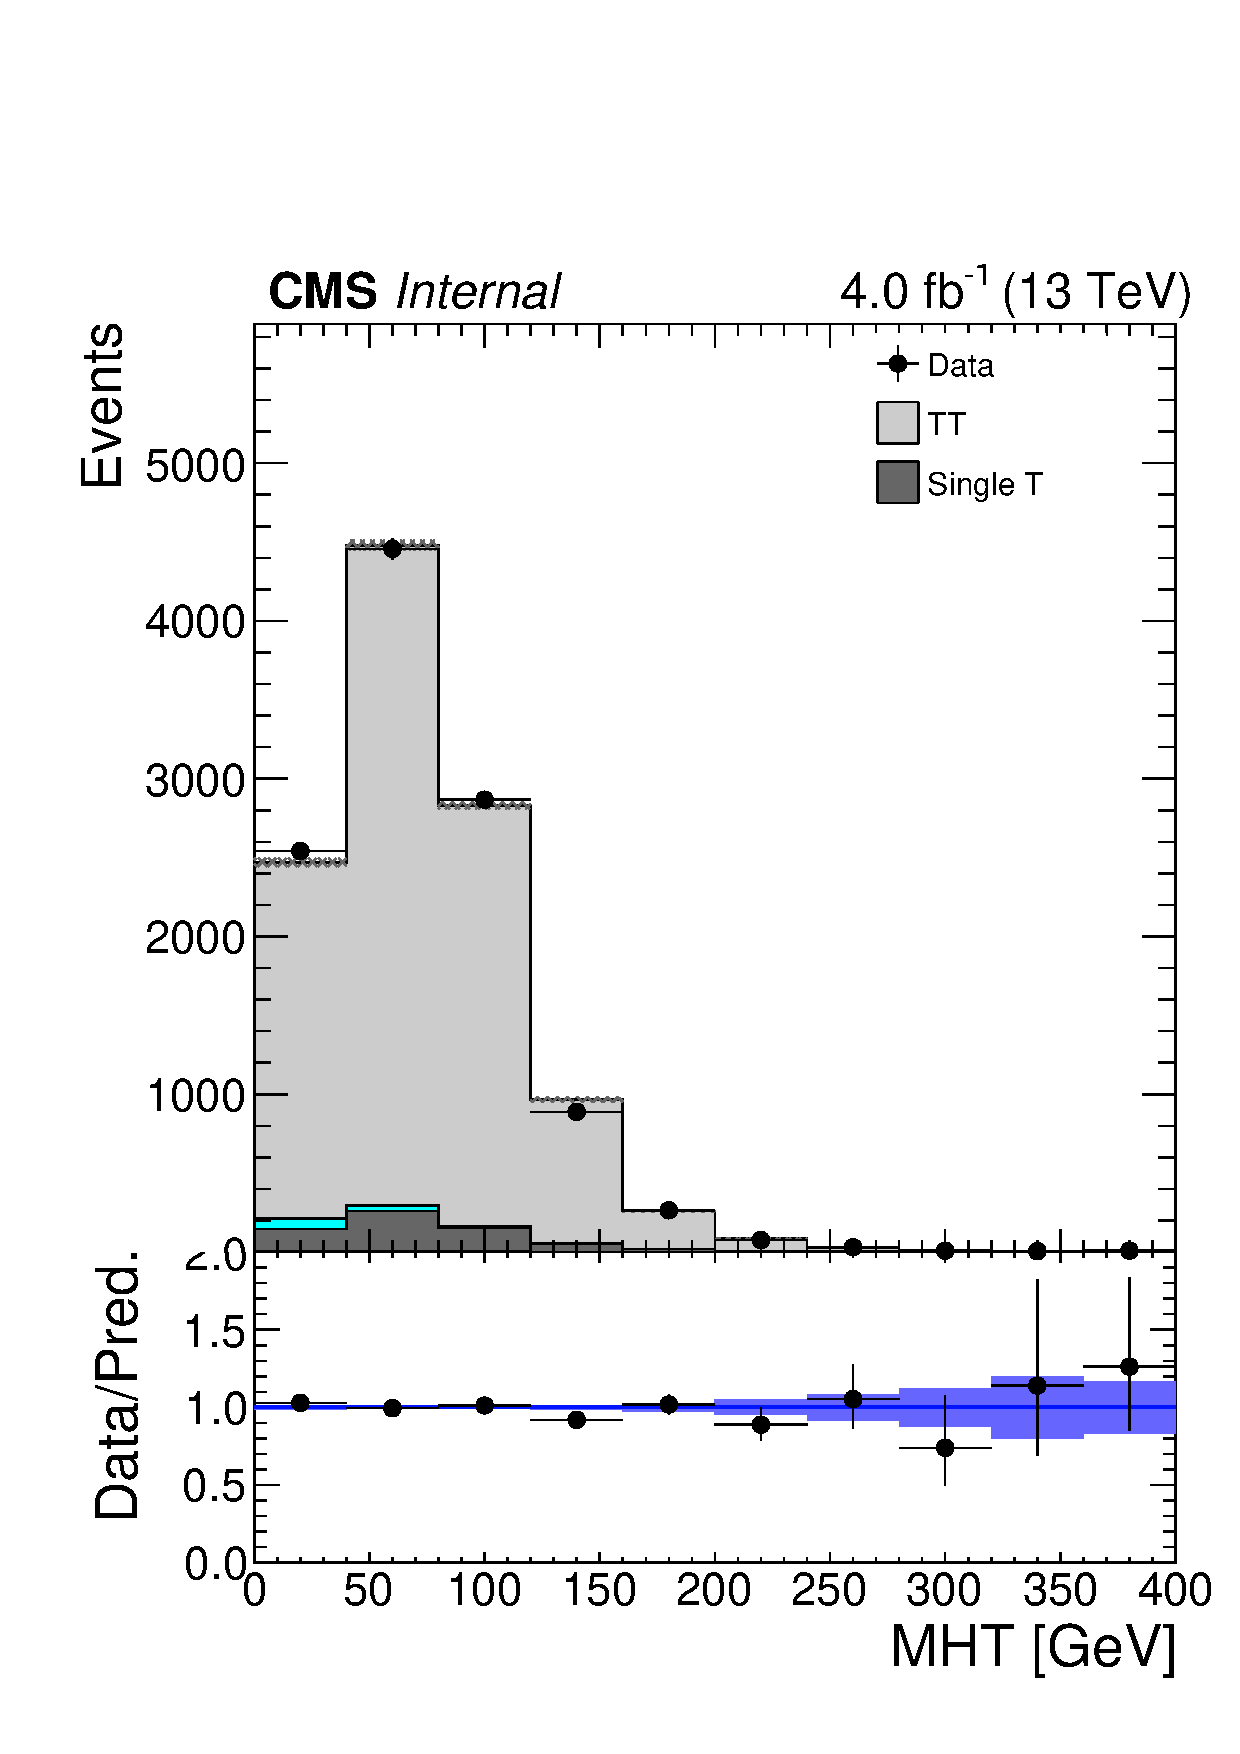
\includegraphics[width=0.32\linewidth]{plots_controlregions/cr_ttbar_data_norm_2j/kinMVA_input_mhtJet25.pdf}\\
%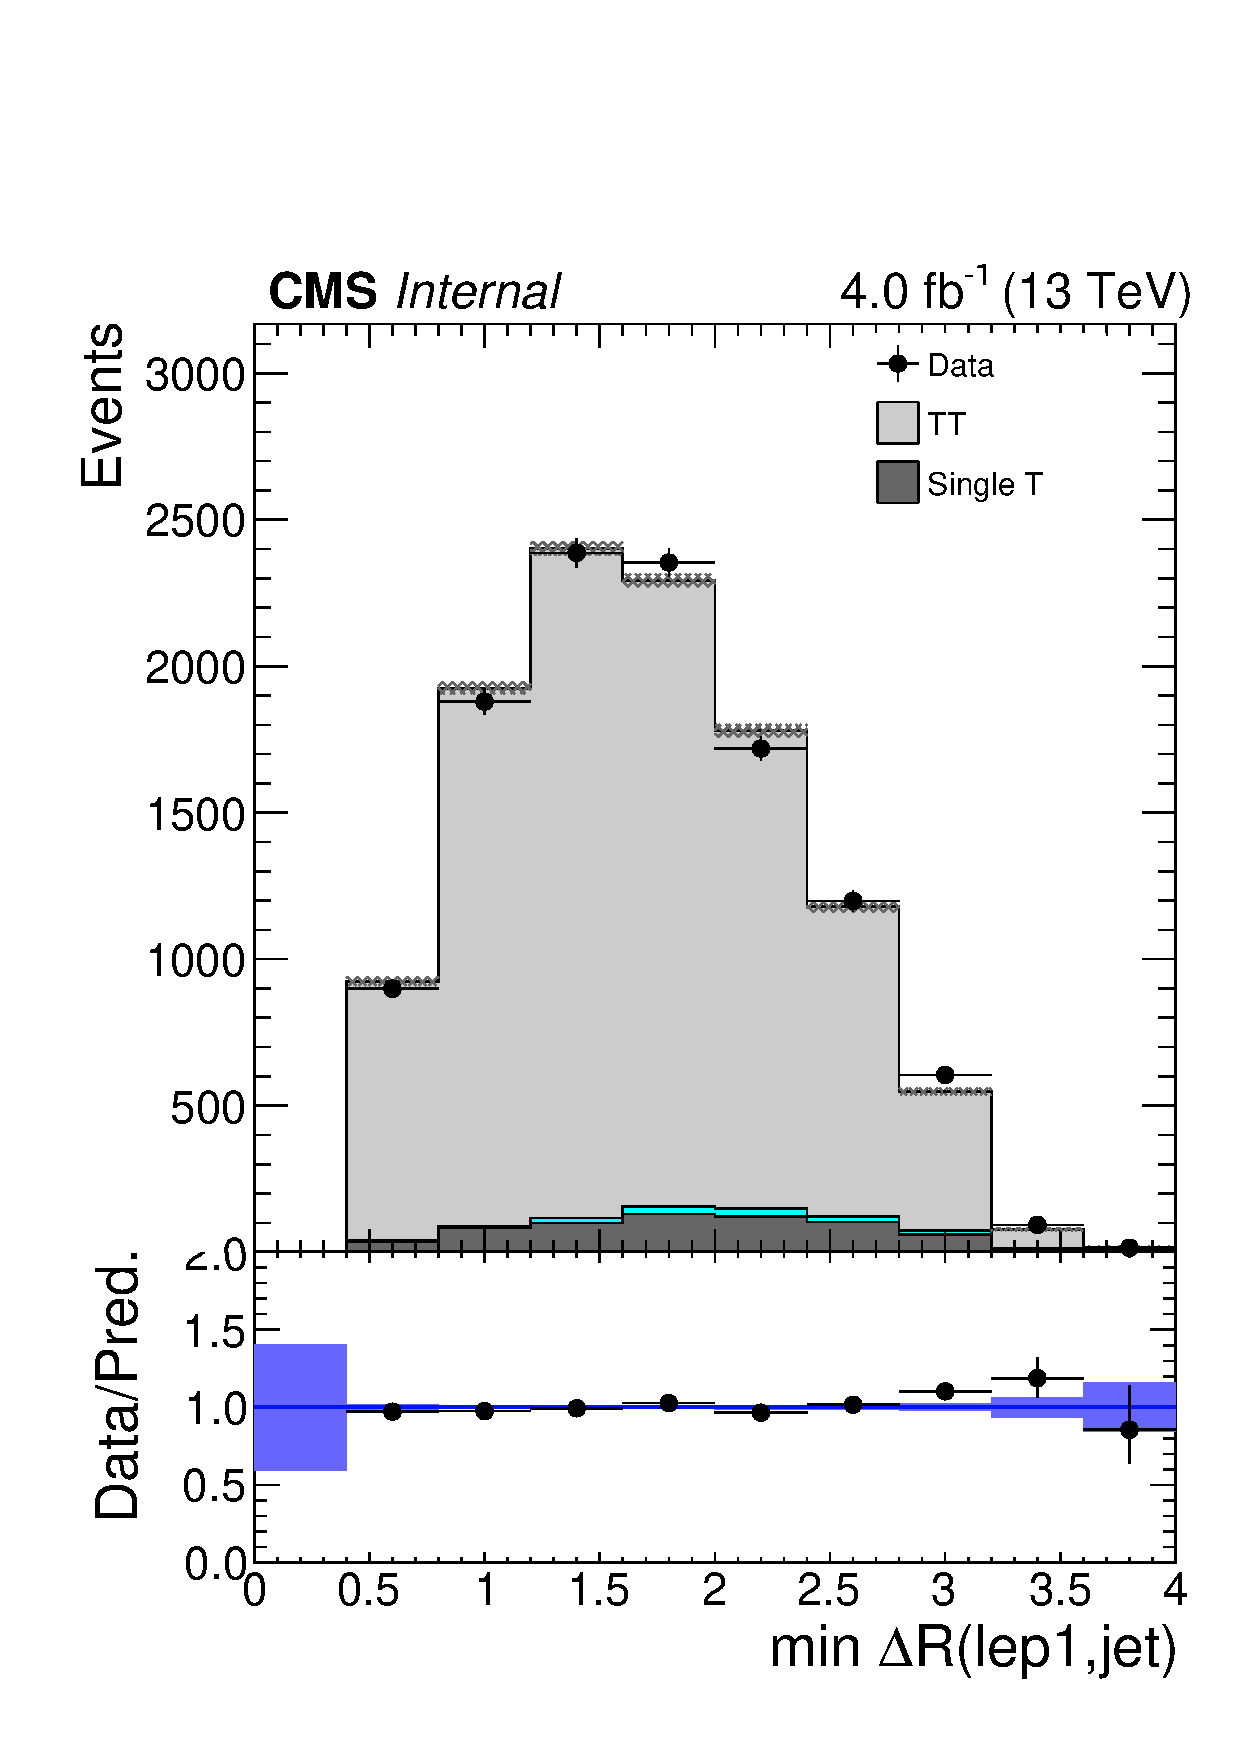
\includegraphics[width=0.32\linewidth]{plots_controlregions/cr_ttbar_data_norm_2j/kinMVA_input_mindr_lep1_jet.pdf}
%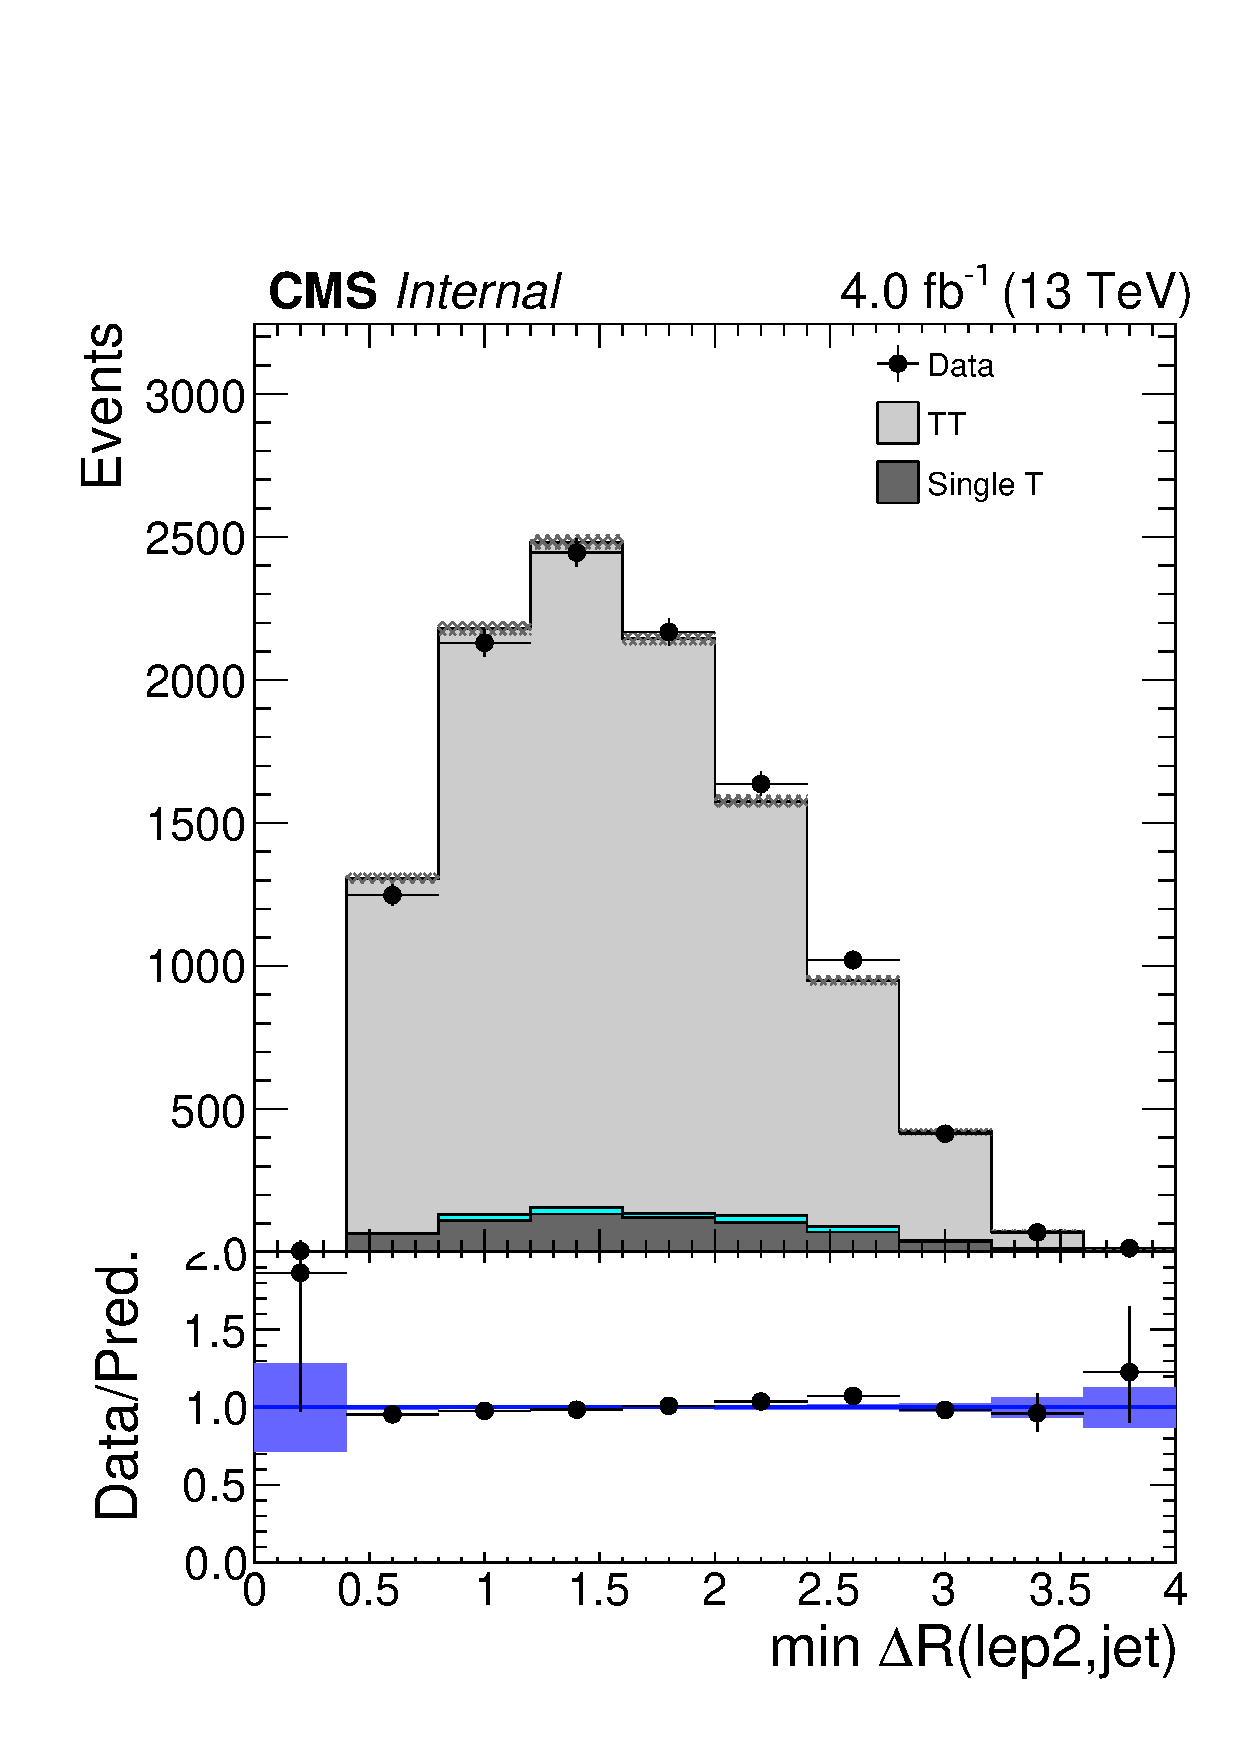
\includegraphics[width=0.32\linewidth]{plots_controlregions/cr_ttbar_data_norm_2j/kinMVA_input_mindr_lep2_jet.pdf}
%\includegraphics[width=0.32\linewidth]{plots_controlregions/cr_ttbar_data_norm_2j/2lep_mll.pdf}\\
%\caption{Data and simulation distributions in the
%$\ttbar\to\Pe^\pm\Pgm^\mp\,\cPqb\cPaqb\,\Pgn\Pagn$ control
%  region, with exactly 2 jets in the final state. Simulation is normalized to data. Uncertainties are statistical only. B-tag scale factors are not applied.
%}
%\label{fig:cr_tt2l_jetbins_norm_2j}
%\end{figure}
%
%\begin{figure}[!htb]
%\centering
%\includegraphics[width=0.32\linewidth]{plots_controlregions/cr_ttbar_data_norm_3j/kinMVA_input_LepGood0_conePt.pdf}
%\includegraphics[width=0.32\linewidth]{plots_controlregions/cr_ttbar_data_norm_3j/kinMVA_input_LepGood1_conePt.pdf}
%\includegraphics[width=0.32\linewidth]{plots_controlregions/cr_ttbar_data_norm_3j/kinMVA_input_MT_met_lep1.pdf}\\
%\includegraphics[width=0.32\linewidth]{plots_controlregions/cr_ttbar_data_norm_3j/kinMVA_input_avg_dr_jet.pdf}
%\includegraphics[width=0.32\linewidth]{plots_controlregions/cr_ttbar_data_norm_3j/kinMVA_input_max_Lep_eta.pdf}
%\includegraphics[width=0.32\linewidth]{plots_controlregions/cr_ttbar_data_norm_3j/kinMVA_input_mhtJet25.pdf}\\
%\includegraphics[width=0.32\linewidth]{plots_controlregions/cr_ttbar_data_norm_3j/kinMVA_input_mindr_lep1_jet.pdf}
%\includegraphics[width=0.32\linewidth]{plots_controlregions/cr_ttbar_data_norm_3j/kinMVA_input_mindr_lep2_jet.pdf}
%\includegraphics[width=0.32\linewidth]{plots_controlregions/cr_ttbar_data_norm_3j/2lep_mll.pdf}\\
%\caption{Data and simulation distributions in the
%$\ttbar\to\Pe^\pm\Pgm^\mp\,\cPqb\cPaqb\,\Pgn\Pagn$ control
%  region, with exactly 3 jets in the final state. Simulation is normalized to data. Uncertainties are statistical only. B-tag scale factors are not applied.
%}
%\label{fig:cr_tt2l_jetbins_norm_3j}
%\end{figure}
%
%\begin{figure}[!htb]
%\centering
%\includegraphics[width=0.32\linewidth]{plots_controlregions/cr_ttbar_data_norm_4j/kinMVA_input_LepGood0_conePt.pdf}
%\includegraphics[width=0.32\linewidth]{plots_controlregions/cr_ttbar_data_norm_4j/kinMVA_input_LepGood1_conePt.pdf}
%\includegraphics[width=0.32\linewidth]{plots_controlregions/cr_ttbar_data_norm_4j/kinMVA_input_MT_met_lep1.pdf}\\
%\includegraphics[width=0.32\linewidth]{plots_controlregions/cr_ttbar_data_norm_4j/kinMVA_input_avg_dr_jet.pdf}
%\includegraphics[width=0.32\linewidth]{plots_controlregions/cr_ttbar_data_norm_4j/kinMVA_input_max_Lep_eta.pdf}
%\includegraphics[width=0.32\linewidth]{plots_controlregions/cr_ttbar_data_norm_4j/kinMVA_input_mhtJet25.pdf}\\
%\includegraphics[width=0.32\linewidth]{plots_controlregions/cr_ttbar_data_norm_4j/kinMVA_input_mindr_lep1_jet.pdf}
%\includegraphics[width=0.32\linewidth]{plots_controlregions/cr_ttbar_data_norm_4j/kinMVA_input_mindr_lep2_jet.pdf}
%\includegraphics[width=0.32\linewidth]{plots_controlregions/cr_ttbar_data_norm_4j/2lep_mll.pdf}\\
%\caption{Data and simulation distributions in the
%$\ttbar\to\Pe^\pm\Pgm^\mp\,\cPqb\cPaqb\,\Pgn\Pagn$ control
%  region, with exactly 4 jets in the final state. Simulation is normalized to data. Uncertainties are statistical only. B-tag scale factors are not applied.
%}
%\label{fig:cr_tt2l_jetbins_norm_4j}
%\end{figure}

%
%%%%%%%%%%%%%%%%%%%%%%%%%%%%%%%%%%%%%%%%%%%%%%%%%%%%%%%%%%%%%%%
\clearpage
%%%%%%%%%%%%%%%%%%%%%%%%%%%%%%%%%%%%%%%%%%%%%%%%%%%%%%%%%%%%%%%

\subsection{\texorpdfstring{$\PW\Z\to3\ell$}{WZ->3l}} \label{sec:WZ control region}
With this control region we want to validate our objects (signal
leptons, $E_{T}^{miss}LD$, jets) in the three lepton final
state.
A sample enriched in $\PW\Z\to3\ell$ events is selected modifying the 3l selection in the following way:
\begin{itemize}
\item the Z veto is inverted, i.e. we require the presence of a pair of loose opposite-sign same-flavor leptons
whose invariant mass is within 10\GeV from the nominal $\Z$ boson mass;
\item we require that no selected jets satisfy the medium working point of the CSV b-tagging discriminator
\end{itemize}
Some distributions are shown in Fig.~\ref{fig:cr_wz}.


\begin{figure}[!htb]
\centering
%\includegraphics[width=0.30\linewidth]{plots_controlregions/cr_wz_data_frdata/lep3_pt.pdf} 
%\includegraphics[width=0.30\linewidth]{plots_controlregions/cr_wz_data_frdata/3lep_worseIso.pdf}
%\includegraphics[width=0.30\linewidth]{plots_controlregions/cr_wz_data_frdata/3lep_worseMVA.pdf}\\
\includegraphics[width=0.30\linewidth]{plots_controlregions/cr_wz_data_frdata/metLD.pdf}
\includegraphics[width=0.30\linewidth]{plots_controlregions/cr_wz_data_frdata/minMllAFAS.pdf}
\includegraphics[width=0.30\linewidth]{plots_controlregions/cr_wz_data_frdata/3lep_mtW.pdf}\\
\caption{Data and simulation distributions in the $\PW\Z\to3\ell$
control region. From left to right: 
the $E_{T}^{miss}LD$, the minimum invariant mass of any $\ell\ell$
 couples, $M_{T}$ of the W boson candidate.}
\label{fig:cr_wz}
\end{figure}


%%%%%%%%%%%%%%%%%%%%%%%%%%%%%%%%%%%%%%%%%%%%%%%%%%%%%%%%%%%%%%%
\clearpage
%%%%%%%%%%%%%%%%%%%%%%%%%%%%%%%%%%%%%%%%%%%%%%%%%%%%%%%%%%%%%%%


\subsection{\texorpdfstring{$\ttbar\Z\to3\ell$}{ttZ->3l}}
\label{sec:ttZto3l}
The prediction for the $\ttbar\Z$ process is tested directly in a trilepton control region
requiring two of the leptons to have the same flavour, opposite electrical charge and the
invariant mass pair of the pair to be within $10\GeV$ of the nominal $\Z$ boson mass.

The definition of the control region differs from the one used for the 3l category of the analysis in the following points:
\begin{itemize}
\item the Z veto requirement is inverted, as described above;
\item the cut on the multiplicity b-tagged jets is tightened, requiring at least two loose and one medium b-tagged jets
\end{itemize}
The background from non-prompt leptons is estimated from data.
Some distributions are shown in Fig.~\ref{fig:cr_ttZ3l}.

\begin{figure}[!htb]
\centering
\includegraphics[width=0.35\linewidth]{plots_controlregions/cr_ttz_data_frdata/lep2_pt.pdf} 
\includegraphics[width=0.35\linewidth]{plots_controlregions/cr_ttz_data_frdata/met.pdf}\\
\includegraphics[width=0.35\linewidth]{plots_controlregions/cr_ttz_data_frdata/nJet25.pdf}
\includegraphics[width=0.35\linewidth]{plots_controlregions/cr_ttz_data_frdata/mZ1.pdf}\\
\caption{Data and simulation distributions in the $\ttbar\Z\to3\ell$
control region. From left to right: the $\pt$ distribution of the
second lepton ordered in $\pt$, the $E_{T}^{miss}$, the number of
central jets with $\pt >$ 25 GeV, the invariant mass of the best $\Z$ candidate.}  
\label{fig:cr_ttZ3l}
\end{figure}


When requiring also the presence of at least four selected jets, as
expected for a fully reconstructed $\ttbar\Z$ event, the control
region for becomes more pure in selecting $\ttbar\Z$ events.
This can be seen in the distributions in Fig.~\ref{fig:cr_ttZ3l4j}.

\begin{figure}[!htb]
\centering
\includegraphics[width=0.35\linewidth]{plots_controlregions/cr_ttz_data_frdata_4j/lep2_pt.pdf} 
\includegraphics[width=0.35\linewidth]{plots_controlregions/cr_ttz_data_frdata_4j/met.pdf}\\
\includegraphics[width=0.35\linewidth]{plots_controlregions/cr_ttz_data_frdata_4j/nJet25.pdf}
\includegraphics[width=0.35\linewidth]{plots_controlregions/cr_ttz_data_frdata_4j/mZ1.pdf}\\
\caption{Data and simulation distributions in the $\ttbar\Z\to3\ell$
control region, with the additional requirement of at least four reconstructed jets.
From left to right: the $\pt$ distribution of the
second lepton ordered in $\pt$, the $E_{T}^{miss}$, the number of
central jets with $\pt >$ 25 GeV, the invariant mass of the best $\Z$ candidate.}  
\label{fig:cr_ttZ3l4j}
\end{figure}



%%%%%%%%%%%%%%%%%%%%%%%%%%%%%%%%%%%%%%%%%%%%%%%%%%%%%%%%%%%%%%%
\clearpage
%%%%%%%%%%%%%%%%%%%%%%%%%%%%%%%%%%%%%%%%%%%%%%%%%%%%%%%%%%%%%%%

   



